%TC:envir temp [] 0
%TC:envir table [] 0
%TC:envir longtable [] 0

%%%%%%%%%%%%%%%%%% USAGE INSTRUCTIONS %%%%%%%%%%%%%%%%%%
% - Compile using LuaLaTeX and biber, unless there is a particular reason not to. Do not use the older LaTex/PDFLaTeX or BibTeX. (The fonts won't work correctly.)
% - Font and the report 'year' must be specified when all \documentclass or the template won't work correctly. (There's no error checking/default cases!)
% - For best performance save images/graphics as PDF files, not as png/jpg/eps. This makes no difference to how images are inserted using \includegraphics.
% - As many further packages as wanted can be loaded. Below are just an example set. Note that template itself loads a number of packages, including hyperref.
% - References are handed using biblatex.
% - Link to the presentation of theses policy: https://documents.manchester.ac.uk/DocuInfo.aspx?DocID=2863



%%%%%%%%%%%%%%%%%% META DATA SETUP %%%%%%%%%%%%%%%%%%
% This is where the document title and author are set. Other details for the title page are set later
% Note that if/when you edit these you may need to 'Recompile from scratch' to get the changes to display in the PDF. (In Overleaf, select the down arrow to the right of the 'Recompile' button)
\begin{filecontents*}{\jobname.xmpdata}
    \Title{COMP30040 Report} 
    \Author{10826115} % should be student number rather than name to help with annoymous marking
    \Language{en-GB}
    \Copyrighted{True}
    % More meta-data fielda can be added here if wanted, see https://ctan.org/pkg/pdfx?lang=en for fields
    \end{filecontents*}
    
    
    %%%%%%%%%%%%%%%%%% DOCUMENT SETUP %%%%%%%%%%%%%%%%%%
    \documentclass{uom_eee_dissertation_casson} 
    
    
    %%%%%%%%%%%%%%%%%% PACKAGES AND COMMANDS %%%%%%%%%%%%%%%%%%
    
    % Packages
    \usepackage{graphicx,psfrag,color} % for postscript graphics files
    \graphicspath{ {./images/} }
    \usepackage{amsmath}               % assumes amsmath package installed
    \allowdisplaybreaks[1]           % allow eqnarrays to break across pages
    \usepackage{amssymb}               % assumes amsmath package installed 
    \usepackage{url}                   % format hyperlinks correctly
    \usepackage{rotating}              % allow portrait figures and tables
    \usepackage{multirow}              % allows merging of rows in tables
    \usepackage{lscape}                % allows pages to be typeset in landscape mode
    \usepackage{tabularx}              % allows fixed width tables
    \usepackage{verbatim}              % enhanced version of built-in verbatim environment
    \usepackage{footnote}              % allows more control over footnote environments
    \usepackage{float}                 % allows H option on floats to force here placement
    \usepackage{booktabs}              % improve table line spacing
    \usepackage{lipsum}                % for adding dummy text here
    \usepackage[base]{babel}           % for proper hypthenation in lipsum sections
    \usepackage{subcaption}            % for multiple sub-figures in a single float
    % Add your packages here
    \usepackage{listings}
    \usepackage{adjustbox}
    \usepackage[bottom]{footmisc}
    \usepackage{longtable}
    \usepackage{tikz}
    \usepackage{varwidth} % For automatic width inside tikz nodes
    \hypersetup{pdfborder={0 0 0}}
    \setlength{\fboxsep}{0pt}
    \setlength{\fboxrule}{0pt}
    
    % Optional: for adding alt-text to images:
    %\usepackage{pdfcomment}            % for alt text for accessibility
    % Then to add images use:
    % \pdftooltip{\includegraphics[width=0.5\textwidth]{image.pdf}}{Alt-text here}
    % This makes the text in the image non-select-able though (assuming it's a vector file)
    
    % Custom commands
    \newcommand{\degree}{\ensuremath{^\circ}}
    \newcommand{\sus}[1]{$^{\mbox{\scriptsize #1}}$} % superscript in text (e.g. 1st)
    \newcommand{\sub}[1]{$_{\mbox{\scriptsize #1}}$} % subscript in text
    \newcommand{\sect}[1]{Section~\ref{#1}}
    \newcommand{\fig}[1]{Fig.~\ref{#1}}
    \newcommand{\tab}[1]{Table~\ref{#1}}
    \newcommand{\equ}[1]{(\ref{#1})}
    \newcommand{\appx}[1]{Appendix~\ref{#1}}
    
    \lstdefinestyle{mystyle}{
        backgroundcolor=\color{gray!10},
        basicstyle=\ttfamily\footnotesize,
        breakatwhitespace=false,
        breaklines=true,
        captionpos=b,
        frame=single,
        keywordstyle=\color{blue},
        commentstyle=\color{green!50!black},
        stringstyle=\color{red},
        numbers=left,
        numbersep=5pt,
        numberstyle=\tiny\color{gray}
    }
    \lstset{style=mystyle}
    
    %%%%%%%%%%%%%%%%%% REFERENCES SETUP %%%%%%%%%%%%%%%%%%
    
    % Setup your references here. Change the reference style here if wanted
    \usepackage[style=ieee,backend=biber,backref=true,hyperref=auto]{biblatex}
    % Note backref=true adds a page number (and hyperlink) to each reference so you can easily go back from the references to the main document. You may prefer backref=false if you need to stick strictly to a given reference style
    
    
    % Fixes which can't be applied in the .cls file
    \DefineBibliographyStrings{english}{backrefpage = {cited on p\adddot},  backrefpages = {cited on pp\adddot}}
    %  \renewcommand*{\bibfont}{\large}
    
    
    % Add more .bib files here if wanted
    \addbibresource{references.bib}
    
    
    
    %%%%%%%%%%%%%%%%%% CUSTOM MODIFICATIONS %%%%%%%%%%%%%%%%%%
    \usepackage{xcolor}
    % Define a custom quote environment
    \renewenvironment{quote}
    {
        \par\setlength{\leftskip}{10pt}
        \begin{tabular}{|p{0.9\linewidth}}  % Vertical bar on the left
        \setlength{\leftskip}{10pt}
        \itshape
    }
    {
        \end{tabular}
        \par
    }
    
    % Define a custom temp environment for placeholders, etc.
    \newenvironment{temp}
    {
        \color{red}  % Set text color to red
        \itshape     % Italicize text for further distinction (optional)
    }
    {
        \normalcolor % Reset text color
    }
    
    \pdfcompresslevel=9
    \pdfobjcompresslevel=3
    
    %%%%%%%%%%%%%%%%%% START DOCUMENT %%%%%%%%%%%%%%%%%%
    
    % Don't edit these lines, title and author are automatically taken from the document meta-data defined above
    \begin{document}
    \makeatletter
    \title{\xmp@Title}
    \studentid{\xmp@Author}
    \makeatother
    
    % Set the below yourself
    \course{Computer Science}  % "Master of Science in" is added automatically
                                                     % Our courses are: Advanced Control and Systems Engineering, Advanced Control and Systems Engineering with Extended Research, Communications and Signal Processing, Communications and Signal Processing with Extended Research, Electrical Power Systems Engineering, Advanced Electrical Power Systems Engineering, Renewable Energy and Clean Technology, Renewable Energy and Clean Technology with Extended Research
    \submitdate{2025}                                  % regulations ask only for the year, not month
    \wordcount{14,993}		                           % use \wordcount{} to set the count, \thewordcount to print in the text
    
    %TC:ignore
    \maketitle
    
    
    %%%%%%%%%%%%%%%%%% LISTS OF CONTENT %%%%%%%%%%%%%%%%%%
    \uomtoc
    % other lists are not required, but can include \uomlof and \uomlot if really want to
    \uomlof
    \uomlot
    
    %%%%%%%%%%%%%%%%%% ABBREVIATIONS %%%%%%%%%%%%%%%%%%%%%
    \phantomsection\addcontentsline{toc}{section}{Abbreviations and Acronyms}
    \section*{Abbreviations and Acronyms}
      % ALWAYS define abbreviations on first use
    
      \begin{description}
        \item[AI] Artificial Intelligence
        \item[API] Application Programming Interface
        \item[CC BY-ND 4.0] Creative Commons Attribution-NoDerivatives 4.0 International Licence
        \item[CC BY-SA 4.0] Creative Commons Attribution-ShareAlike 4.0 International Licence
        \item[CD] Compact Disc
        \item[CDPA] Copyright, Designs and Patents Act 1988
        \item[CLK] Clock (regular pulses used for quadrature rotary encoding)
        \item[CNN] Convolutional Neural Network
        \item[CV] Computer Vision
        \item[DRM] Digital Rights Management 
        \item[DT] Data (offset pulses used for quadrature rotary encoding)
        \item[EN] Enable
        \item[GDPR] General Data Protection Regulation
        \item[GUI] Graphical User Interface
        \item[GPIO] General-Purpose Input/Output
        \item[GPU] Graphical Processing Unit
        \item[HTTP] Hypertext Transfer Protocol
        \item[HTTPS] Secure Hypertext Transfer Protocol
        \item[LP] Long Play
        \item[ML] Machine Learning
        \item[MP3] Moving Picture Experts Group (MPEG) Audio Layer 3
        \item[OCR] Optical Character Recognition
        \item[OS] Operating System
        \item[PWM] Pulse-Width Modulation
        \item[REST] Representational State Transfer
        \item[RPi] Raspberry Pi
        \item[RPiOS] Raspberry Pi OS (formerly Raspbian)
        \item[RPM] Rotations per Minute
        \item[SBC] Single-Board Computer
        \item[SDK] Software Development Kit
        \item[SRP] Single Responsibility Principle
        \item[SSE] Server-Sent Events
        \item[SW] Switch (the live connection of a button circuit) 
        \item[ToS] Terms of Service
        \item[TOU] Terms of Use
        \item[TPU] Tensor Processing Unit 
        \item[UML] Unified Modeling Language
        \item[URI] Uniform Resource Identifier
        \item[UX] User Experience
      \end{description}
    
    %%%%%%%%%%%%%%%%%% ABSTRACT %%%%%%%%%%%%%%%%%%%%%%%%%%
    \begin{abstract} % put abstract here. Limit is 1 page.
    
        This project develops an innovative solution that merges the physical and digital music experience by enabling vinyl records to be digitally streamed through image recognition. Leveraging machine learning, the system identifies physical album covers and retrieves corresponding audio tracks from Spotify. Built on a Raspberry Pi 5 platform, it provides users the tangible experience of vinyl while offering the convenience of digital playback. The project's objectives include addressing limitations inherent to vinyl, such as equipment fragility and playback inconvenience, and targeting vinyl enthusiasts who value both aesthetics and usability. Experimentation with various neural network models resulted in a top-1 accuracy of 91.18\%, average response times under four seconds, and 71.5\% code coverage. Qualitative testing confirmed the system's intuitive interface and nostalgic appeal. Challenges addressed include reliable image recognition, legal and ethical concerns, and robust integration of hardware and software components. Evaluation shows the solution effectively enhances the usability and appeal of vinyl collections.
    
    \end{abstract}%
    \clearpage
    
    
    
    %%%%%%%%%%%%%%%%%% DECLARATIONS %%%%%%%%%%%%%%%%%%
    \uomdeclarations % Don't need unless final thesis
    
    
    
    %%%%%%%%%%%%%%%%%% ACKNOWLEDGEMENTS %%%%%%%%%%%%%%%%%%
    \begin{uomacknowledgements}
    I would like to extend my gratitude to the noble mahogany tree, whose sacrifice provided not only the material for a Welsh love spoon -- by which I proposed and became engaged to my beloved fiancée -- but also the offcuts that found purpose in the physical interface of this project. Your contribution to both my personal and academic life has been truly invaluable.
    
    Also, to my close friend Joshua Bond's dissertation \cite{jdbond}, which I have yet to finish reading -- but I am sure it is great.
    \end{uomacknowledgements}
    
    %TC:endignore
    
    %%%%%%%%%%%%%%%%%% SECTION 1 %%%%%%%%%%%%%%%%%%
    \section{Introduction}
    
        \subsection{Background and motivation}
    
            The resurgence of vinyl records -- recently reaching decade-high sales \cite{geraghty2023uk_vinyl_sales} -- presents both opportunity and challenge: growing interest among younger listeners and collectors \cite{Trapp2023}. Yet, despite their renewed popularity, vinyl records require specialised equipment, knowledge of different record sizes and playback speeds, and accessories such as 33–45 adapters for discs with larger centre holes (see Figure~\ref{fig:vinylSizes}) -- posing practical barriers to modern listeners.
    
            \begin{figure}[htbp]
                \centering
                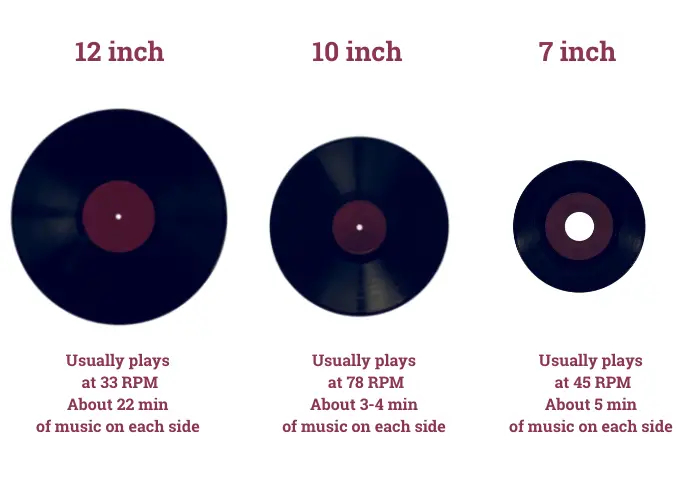
\includegraphics[width=0.8\linewidth]{images/33vs45.jpg}
                \caption{Overview of vinyl record sizes and their corresponding playback speeds.}
                \caption*{Sourced from \href{https://notesonvinyl.com/the-difference-between-33-vs-45-vinyl/}{Notes On Vinyl}. Reproduced under UK fair dealing provisions for non-commercial academic use.}
                \label{fig:vinylSizes}
            \end{figure}
    
            Combining digital and physical media provides an attractive solution to these challenges by merging the tangible appeal of vinyl with the convenience and accessibility of digital music streaming. Such an integration maintains the emotional and tactile connection that many listeners appreciate in physical collections \cite{Liu2020}, while offering the ease of digital technologies. Given current consumer interests and technological advancements, this hybrid approach is timely and relevant.
        
        \subsection{Aims and objectives}
    
            This project aims to resolve key limitations of traditional vinyl playback by:
            \begin{itemize}
                \item Identifying and addressing practical limitations of analogue systems;
                \item Designing a hybrid physical–digital playback system;
                \item Enabling users to stream music by scanning album covers;
                \item Evaluating performance through quantitative and qualitative testing;
            \end{itemize}
    
            The full goals and evaluation methodology, including test datasets, user testing approach, and success criteria, is detailed in the Design Section's Requirements Analysis~(\ref{sec:reqany}).
    
            Intended users include vinyl enthusiasts, collectors, and casual listeners who appreciate vinyl's tangible and aesthetic aspects but desire greater convenience. The project addresses a gap where physical collections are underutilised due to traditional playback inconvenience.
        
        \subsection{Scope}
    
            In scope for this project is the development of an application that uses image recognition technology -- such as machine learning (ML) and Optical Character Recognition (OCR) -- to identify vinyl records and retrieve corresponding digital tracks from streaming platforms like Spotify. The solution is built on a Raspberry Pi 5-based hardware platform, integrating both physical and digital user interfaces.
    
            Out of scope elements include extensive hardware customisation beyond essential playback functionality, support for every possible streaming service, and creation of original music databases. The focus is on Spotify's streaming capabilities -- due to its widespread adoption and available Application Programming Interface (API) support -- whilst still maintaining flexibility and the ability to change APIs easily, if desired.
        
        \subsection{Challenges}
    
            As demonstrated in prior work, convolutional neural networks are effective for image recognition across varied domains \cite{cnnsforimagerecognition, imagenetclasscnn}, but even these face limitations. The primary challenges anticipated include accurately identifying album artwork using ML techniques, managing legal and ethical concerns related to copyrighted album covers, and effectively integrating multiple technologies -- such as hardware components, web APIs, and neural networks -- into a cohesive system. Balancing usability and technical robustness is also a challenge.
        
        \subsection{Report structure} % ROADMAP
        
            This report consists of seven chapters:
            \begin{description}
                \item[Chapter 1] introduces the project, its motivations, objectives, and challenges.
                \item[Chapter 2] presents the background and literature review, discussing existing technologies and relevant research informing design choices.
                \item[Chapter 3] details the project's design decisions, system architecture, and chosen technologies.
                \item[Chapter 4] describes the implementation process, outlining how design considerations translated into practical development.
                \item[Chapter 5] presents the outcomes of the implemented solution, showcasing software and hardware artefacts.
                \item[Chapter 6] evaluates the project's effectiveness, usability, and impact, including comparisons to existing systems.
                \item[Chapter 7] summarises conclusions, identifies project limitations, and suggests avenues for future development.
            \end{description}
    
            While not strictly chronological, the chapters follow the stages of the development process.
    
    %%%%%%%%%%%%%%%%%% SECTION 2 %%%%%%%%%%%%%%%%%%
    \section{Background and Literature Review} % LITERATURE REVIEW / BACKGROUND
      % [ ] summary of similar systems
      % [ ] explanations of concepts relied on later
      % [ ] advanatges and disadvantages of approaches
      % [ ] highlight problems I will improve
      % [ ] cite all references
    
      \subsection{Overview of Related Systems}
    
        Whilst the creation of a digitised turntable software is a rather novel idea, it is important to consider where this sits in the existing landscape; to understand technologies and design decisions in similar projects.
      
        \subsubsection{Vinyl Systems}
    
            \begin{quote}
                ``Vinyl is back!'' \cite{bechhofervttspec}
            \end{quote}
            
            In 2023, UK vinyl sales reached their highest level since 1990 \cite{geraghty2023uk_vinyl_sales}, confirming the ongoing ``vinyl revival'' \cite{vinylRevival} (see Figure~\ref{fig:vinyl_sales}). Initially dismissed as a short-term trend when it emerged in 2008-2009, this resurgence has persisted, highlighting a renewed interest in physical music formats. Understanding the motivations behind this revival is crucial for informing design decisions, particularly from a User Experience (UX) perspective, as vinyl collectors constitute a key target audience.
            
            \begin{figure}[htbp]
                \centering
                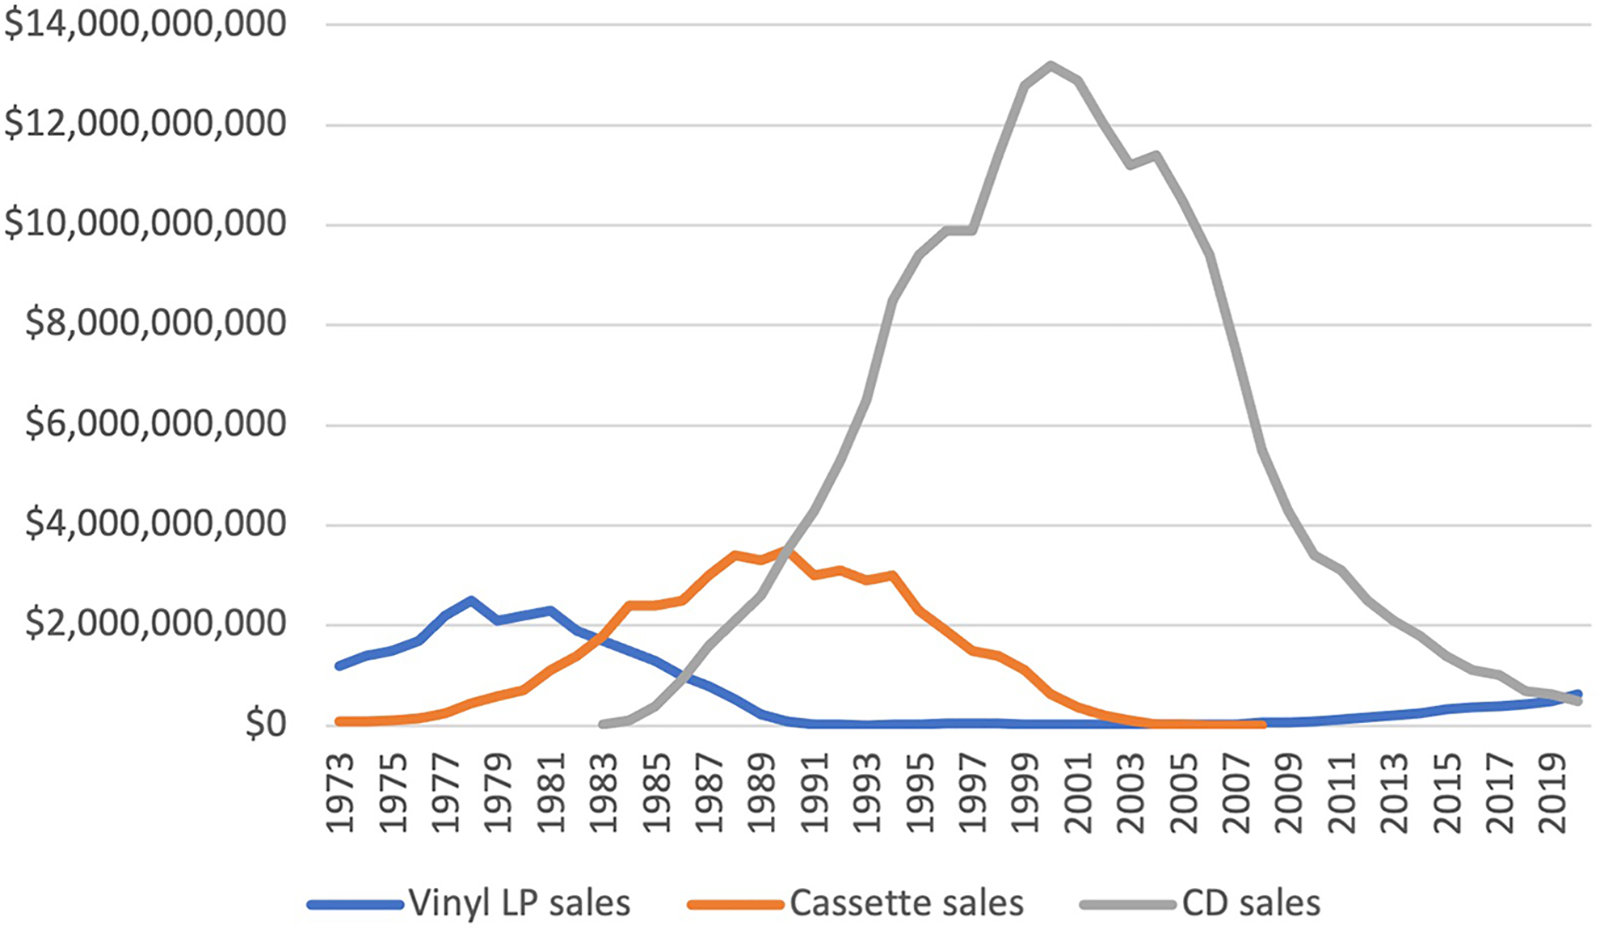
\includegraphics[width=\linewidth]{images/vinyl_sales_2023.png}
                \caption{Vinyl LP, Cassette, and Compact Disc (CD) Sales Revenue (1973–2020).}
                \caption*{Sourced from Journal of Popular Music Studies \cite{vinylRevival}. Reproduced under UK fair dealing provisions for non-commercial academic use.}
                \label{fig:vinyl_sales}
            \end{figure}
    
            Although now taken for granted, records -- and their predecessors, Edison's cylinders -- transformed music from an ephemeral experience into a reproducible medium. Before recording technology, music was transient and confined to its place and time of performance, unable to be stored or shared beyond a live setting. While compositions could be transcribed into musical notation, each unique performance could never be heard again once it ended, unlike with visual art, where many original works from as far back as antiquity still survive \cite{jdbond}.
    
            This revolution in music consumption not only shaped the modern music industry but also cemented vinyl's cultural significance. By making music ownable and replayable, it changed the way people engaged with it, fostering a more personal and enduring connection. Its enduring appeal, even in the digital age, suggests that its value extends beyond convenience, tapping into a deeper connection with music as a tangible experience.
    
            % Aesthetics
            \paragraph{Aesthetics and Emotional Appeal}
                % nostalgia, vibes
    
                Though nostalgia is widely recognised as a key driver of vinyl's revival; it varies by age group. Gotting \cite{Gotting2021} shows that engagement peaks among both older listeners, who have direct sentimental ties to the medium, and younger adults, who view vinyl as a culturally rich artefact. Liu \cite{Liu2020} adds that this appeal is partly a reaction to the disposability of digital listening with users seeking more focus and ritual.
    
                Historically, music was a shared, physical experience: families gathered around a single record player, and listening required attention. Today, however, listeners often engage in fragmented, solitary consumption \cite{historyandrevivalofvinyls}. The skip-anything convenience of streaming has reduced music to background noise for many users. Vinyl's tactile nature and unskippable format offer a counter-experience -- one that demands physical presence and invites emotional connection.
    
                This resurgence is not only aesthetic but communal. Platforms like Reddit's r/Vinyl\footnote{\url{https://www.reddit.com/r/vinyl/}} (with over 2.2 million members as of 2025) show that people are forming identity and community around the medium itself. Mall \cite{vinylRevival} and others argue that vinyl offers a kind of cultural resistance: a slower, more deliberate engagement in an increasingly digital and transient world.
          
              % Ownership
              % Physicality
            \paragraph{Physicality and Ownership} % or MATERIALITY; general ethics
    
                Digital ownership is increasingly precarious, with users buying licences rather than assets \cite{verge2024steam_license}. This transition has upset many people, with there being many calls to bring back genuine ownership \cite{stanton2024gamers_pushback}, with legislation even being passed in California to make this fact more transparent to consumers \cite{california2024ab2426}.
    
                If a streaming vendor stops serving a particular piece of music, then that album can be lost to the public forever \cite{polygon2024cartoon_network_delisting}. However, if a consumer actually owns the physical discs or digital audio files, then they can ensure that they can listen to their audio, regardless of whatever licensing disputes may lead to the removal of digital media in the future (see \cite{bains2022lotr_strategy}).
    
                Furthermore, there are also concerns that streaming platforms often provide artists with minimal financial compensation, leading some consumers to purchase physical media as a means of direct support \cite{historyandrevivalofvinyls}. This means that there is a demographic of people who both own physical vinyls, but still make use of digital streaming services. Many even purchase vinyls without owning a player \cite{Trapp2023}. In addition, the act of gaining a physical good in support of an artist can even result in a psychological feeling of proximity to their idol \cite{historyandrevivalofvinyls}.
                
                Additionally, vinyl's finite nature contrasts with the boundless availability of digital tracks, making collections feel more meaningful and curated.
    
            % Audiophiles
            \paragraph{Audiophilia and Sound Quality}
    
                Another significant factor is the quality of the music being offered.
    
                \begin{quote}
                    \textbf{audiophile}: a person who is especially interested in high-fidelity sound reproduction. \cite{audiophile2025}
                \end{quote}
    
                % quality
                Perceptions of vinyl's superior audio quality often stem from early digital compression issues, rather than objective fidelity differences. For example, early MP3 encodings of minimal tracks such as ``Tom's Diner'' exposed compression artefacts \cite{maguire2014ghost}. Although modern digital formats objectively outperform vinyl in fidelity -- especially in terms of bit depth and dynamic range -- user perception may not align with these metrics. In low-bandwidth environments, highly compressed audio can degrade noticeably, sometimes sounding worse than a clean vinyl pressing. This contrast is crucial for hybrid systems, where listeners may subconsciously associate streaming with lower quality, reinforcing vinyl's perceived authenticity.
    
                Additionally, vinyl is susceptible to scratches and physical deformities which affect the playback quality. Vinyl enthusiasts appreciate the medium's imperfections, which are thought to add warmth and character. No two discs sounds exactly the same. This creates a sense of personal ownership with vinyls -- not only does the consumer own the physical disc itself, but they own their precise and unique version of it.
    
                It is important to note that many contemporary vinyl releases originate from digital masters, meaning potential losses in fidelity depend on how well an album is adapted to the format. Several inherent limitations affect vinyl playback, including: duration constraints, due to physical disk size; track sequence issues, as resolution gradually degrades towards the inner grooves; and RIAA\footnote{Recording Industry Association of America} equalisation, which alters frequency response to accommodate physical limitations of the medium \cite{engineeringvinyls}. Additionally, stereo information handling differs from digital formats, as vinyl relies on lateral and vertical groove modulation, which can introduce crosstalk and phase issues \cite{engineeringvinyls}. These factors, if not carefully managed during production, may compromise the listening experience. Modern tracks often sound better in digital.
    
            \paragraph{Conclusion}
                While digital audio services offer notable convenience, the enduring vinyl revival demonstrates that many users still value tangible, nostalgic experiences. Nostalgia and charm play a crucial role in this appeal, making it essential to design with these emotional connections in mind. By combining the strengths of both physical and digital formats, a system can provide a richer, more meaningful user experience that aligns with modern consumption habits while preserving the authenticity and personal connection that vinyl enthusiasts cherish. A significant portion of consumers actively engage with both streaming services and physical media, indicating that a hybrid approach has a viable audience.
    
        \subsubsection{Image Recognition}
    
            % Y. LeCun and Y. Bengio, 1995, "Convolutional Networks for Images, Speech, and Time-Series". Brain theory neural networks, vol. 3361
    
            Image recognition is the creation of software and tools which can be used to identify objects, places, people, etc. in digital images, which has existed since at least 1946 \cite{hall1979computer}. The field has rapidly evolved with advancing technology \cite{imagenetclasscnn}, and is still be redefined in the present day, particularly with the arrival of ML approaches, with new implementations being utilised across the field (e.g. \cite{RAMPRASAD2025100556}, 2025).
    
            \paragraph{Traditional Methods}
            
                Before the advent of deep learning, image recognition primarily relied on manually crafted feature extraction techniques. Classical methods included edge detection, template matching, and statistical pattern recognition. Notable feature descriptors such as Scale-Invariant Feature Transform (SIFT), Speeded-Up Robust Features (SURF), and Histogram of Oriented Gradients (HOG) played a significant role in object detection and classification \cite{pal2001pattern}. That said, these approaches were often limited by their inability to generalise across variations in lighting, scale, and occlusions. The ImageNet Large Scale Visual Recognition Challenge\footnote{https://www.image-net.org/challenges/LSVRC/} (ILSVRC) served as a benchmark for evaluating the effectiveness of traditional and emerging techniques \cite{russakovsky2015imagenetlargescalevisual}.
            
            \paragraph{Emergence of Convolutional Neural Networks}
            
                The introduction of convolutional neural networks (CNNs) marked a paradigm shift in image recognition. Early work, such as LeNet-5, demonstrated CNNs' potential \cite{726791}, but it was the breakthrough of AlexNet in the 2012 ImageNet competition that solidified their dominance \cite{imagenetclasscnn}. Subsequent architectures, including VGG, ResNet, and EfficientNet, further improved performance by introducing deeper networks, residual connections, and optimised convolutional layers \cite{deppcnnsforimagerecognition}. These advancements enabled significant improvements in tasks such as object detection, facial recognition, and medical image analysis.
    
                In the context of vinyl cover art recognition, CNNs offer a powerful solution for identifying album artwork despite variations in artistic style, degradation, and distortions. Although, a key challenge in training CNNs for this task is the limited availability of labelled datasets. Unlike large-scale image classification datasets like ImageNet, curated datasets for album cover recognition remain relatively small. To address this limitation, data augmentation techniques -- such as random cropping, rotation, colour jittering, and synthetic distortions -- help improve model robustness by simulating real-world variations \cite{LIN2025102660}. Even further, research has been done recently into using stable diffusion techniques to facilitate fully artificial data augmentation, with generative Artificial Intelligence (AI) \cite{Alimisis2025}. However, larger augmented datasets increase computational demands, making optimisation for Graphics Processing Units (GPUs) or Tensor Units (TPUs) essential for efficiency.
    
            \paragraph{Multi-Headed Networks and Consensus-Based Recognition}
    
                A limitation of conventional CNN models in image recognition is their reliance on a single decision pathway, which can lead to misclassifications when dealing with visually similar or degraded images. One approach to mitigate this issue is the use of multi-headed neural networks, where multiple CNN branches extract different features and contribute to a consensus decision. This technique allows the network to assess multiple aspects of the image, like texture, colour, and structure before making a final classification \cite{Zheng2017}. 
            
                By integrating multi-headed architectures with ensemble strategies, models can achieve higher classification accuracy and robustness, particularly when handling ambiguous or visually noisy inputs. This method has been successfully applied in fine-grained classification tasks and could be adapted for vinyl cover recognition by leveraging multiple specialised feature extractors that assess distinct album cover characteristics.
    
            \paragraph{Current `State of the Art'}
    
                Visual transformers currently represent the state-of-the-art in image classification, significantly outperforming traditional CNNs on large datasets \cite{dosovitskiy2020vit}. Albeit, their performance heavily depends on large-scale data availability; for limited or specialised datasets, such as vinyl cover recognition, transformers may perform poorly or be impractical. Thus, CNN-based architectures or hybrid approaches remain more suitable in scenarios with smaller, niche datasets.
    
                A key challenge is ensuring models generalise effectively to unseen data, avoiding overfitting. Techniques like dropout, which randomly deactivate neurons during training, improve robustness by preventing reliance on specific features. Additionally, splitting datasets into training, validation, and test subsets enables monitoring model generalisation, though careful consideration is required to balance partition sizes and representativeness, whilst also avoiding biases.
    
        \subsection{Legal and Ethical Considerations}
    
          The training and use of ML models for image classification requires the acquisition and processing of data, which, in order to effectively handle the cover art of existing albums, necessitates obtaining and using their copyrighted artworks. This raises both legal and ethical concerns, particularly regarding compliance with UK copyright law. This section examines the legal basis for dataset usage, fair dealing exemptions, and the ethical implications of using copyrighted material in an academic AI project.
    
              \subsubsection{Copyright Law and Fair Dealing}
                  % explain copyright law
                  Under the \textit{Copyright, Designs and Patents Act 1988} (CDPA) \cite{cdpa1988}, creative works, including album covers, are protected from unauthorised use, reproduction, distribution, and modification.
          
                  % introduce fair dealing
                  Even so, UK law also provides a key exception known as Fair Dealing, which allows limited use of copyrighted material under specific conditions, for a very limited scope of use. Importantly, it is not a rigid rule but a context-dependent legal doctrine, evaluated on a case-by-case basis. The law does not explicitly define what qualifies as fair dealing; courts assess reasonableness based on context.
                  
                  One of the most relevant exemptions is non-commercial research, as outlined in \textit{Section 29(1)} of the CDPA:
                  \begin{quote}
                      Fair dealing with a work for the purposes of research for a non-commercial purpose does not infringe any copyright in the work provided that it is accompanied by a sufficient acknowledgement. \cite{cdpa1988}
                  \end{quote}
    
                  This indicates that non-commercial academic research can be exempt from copyright infringement if proper attribution is provided. That said, the applicability of this exemption depends on further and additional factors, such as the amount of material used and its impact on the copyright holder's market.
    
              % 1. Using a dataset to create a model
              \subsubsection{Use of Artworks in Model Training}
              
                  Album covers are protected by copyright as highly creative works. Any reproduction or modification is typically restricted without permission from the copyright holder. As such, the threshold for qualifying as fair dealing is high, when dealing with such artwork. However, training a classification model may qualify for fair dealing, provided certain conditions are met.
    
                  A key legal question is whether ML training qualifies as ``\textit{computational analysis}'' under \textit{Section 29A} of the CDPA, which states:
                  \begin{quote}
                      (1) The making of a copy of a work by a person who has lawful access to the work does not infringe copyright in the work provided that --
                  
                          (a) the copy is made in order that a person who has lawful access to the work may carry out a computational analysis of anything recorded in the work for the sole purpose of research for a non-commercial purpose, and
                          
                          (b) the copy is accompanied by a sufficient acknowledgement (unless this would be impossible for reasons of practicality or otherwise). \cite{cdpa1988}
                  \end{quote}
    
                  This expresses that there is a strong argument for legal use of copyrighted materials in creating a computational model which classifies data by comparisons of analytically-derived embeddings.
    
                  It is, nevertheless, important to consider whether image processing qualifies as analysis under this law or whether this interpretation is too broad, given that past applications of computational analysis have predominantly involved text, and that image processing of this kind is still relatively new. Since there is no clear legal precedent on this specific topic (with changes being in the process of being made \cite{guardian2024uk_ai_copyright}), further legal clarification over the next few years will be necessary to definitively confirm or deny its applicability to image-based AI models. But, in the time before then, it can be used as a basis.
    
                  It also reiterates the need for attribution, but, notably states that this is only required in cases where it is feasibly practical.
    
                  Given these factors, classification likely qualifies under Fair Dealing because the model does not generate new images but merely classifies existing ones. This distinction is important, especially given recent scrutiny of generative AI models like OpenAI's \textit{DALL·E} \cite{times2025christies_ai_auction, guardian2025ai_art_auction}, which create derivative works rather than merely labelling.
    
                  None of this is clear-cut, though, as this is still an uncertain time with the law not having been stabilised after the emergence and mass adoption \cite{bick2024rapid} of these new technologies. It is worth noting, however, that there are currently proposals for UK law to explicitly allow the use of copyrighted materials in such cases \cite{guardian2024uk_ai_copyright}, whereas, in the US, there is starting to be legal prescendent of cases winning on the basis \cite{apnews2025thomson_reuters_ai_case} of AI agents using copyrighted data.
    
              % 2. Sourcing said dataset
              \subsubsection{Legal Compliance in Dataset Sourcing}
    
                  Beyond Fair Dealing considerations, data sourcing must be legally compliant. According to \textit{Section 29A} \cite{cdpa1988}, only individuals with lawful access to copyrighted works may use them for computational analysis. Therefore, it is essential to determine how these images can be legitimately acquired.
    
                  ML models must fully process training images in their entirety to generate a model. This requires the whole image to be either stored persistently (on disk) or temporarily (in memory). Even if handled in chunks, the full image is processed by the model. \textit{Section 28A} outlines more leniency for cases where only temporary copies are stored, for lawful access.
    
                  It is also important to consider if entire images are required, as opposed to only sections of them. If it would be possible to achieve the desired result using only subsets of the acquired dataset, then more data would be stored and used than is justified. The legal precedent \textit{Ashdown v Telegraph Group Ltd (2002)}, highlights that:
    
                  \begin{quote}
                      The third most important factor is the amount and importance of the work that has been taken . . . in some circumstances the taking of an excessive amount, or the taking of even a small amount if on a regular basis, would negative fair dealing. \cite{tmlocad}
                  \end{quote}
    
                  Thus, ensuring only necessary data is used is critical for compliance.
    
                  % 3. ToS compliance
                  In addition to just the handling of the data, its source must also be considered. There are three methods by which the training dataset could be acquired: by fetching data from an API, by scraping the data from the web, or, by manually taking the required photos (either personally, or through crowd-sourcing). Realistically, the first two options are most practically feasible.
    
                  There are many vendors of the cover arts of music albums. Notably, music vendors (such as \textit{Spotify}) and music collection and review sites (such as \textit{Discogs}) provide the album arts in a structured format where the artworks are synchronised with the albums which they belong to. Although, due to the recent boom of generative AI models - and the controversy surrounding them \cite{apnews2025mccartney_ai_warning} - many vendors have explicitly prohibited the use of their data for machine learning in their Terms of Services.
    
                  % specific examples should probably be discussed under 'Design'
                  \begin{quote}
                      Do not use the Spotify Platform or any Spotify Content to train a ML or AI model or otherwise ingest Spotify Content into a machine learning or AI model.
                  \end{quote} \cite{spotifyDevPolicy} (III.14)
                  \begin{quote}
                      Do not misuse the Spotify Platform, including by i. using the Spotify Platform or any Spotify Content to train a machine learning or AI model or otherwise ingesting Spotify Content into a machine learning or AI model;
                  \end{quote} \cite{spotifyDevTerms} (IV.2.a.i)
                  \begin{quote}
                      [Discogs] strictly prohibit (1) the development of any software program, including, but not limited to, training a machine learning or artificial intelligence (AI) system using the Service content
                  \end{quote} \cite{discogsToS} (LICENSE AND SITE ACCESS)
    
                  However, if a site has more permissive policies, allowing the training of AI models, then, as long as the images are handled appropriately, they can be lawfully accessed and used.
    
              \subsubsection{Ethical Considerations}
              % Even if it's legally permissible, is it ethically responsible?
              % Does it impact the commercial success of artists?
              % Transparency & attribution concerns.
    
                  While legality is addressed under Fair Dealing, ethics requires further consideration. Even when lawful, using copyrighted artwork involves reproducing creative works, and this should be done with care and respect for the artists' rights and livelihoods \cite{heikkila2022ai_art}.
    
                  Most significantly, it is worth noting that this AI model is not generative (which is where most of the recent controversies stem from \cite{apnews2025mccartney_ai_warning}), and therefore, instead of producing its own artworks based off of the images fed to it, it simply classifies them by labelling them with its prediction of their corresponding album. Therefore, while the model is technically derived from artists' works, it does not generate new content or compete with them -- unlike generative agents \cite{times2025photographer_ai_copy} -- and so is unlikely to negatively impact their commercial success. If anything, it can be argued that this system should benefit them, by encouraging the purchasing of physical media, and garnering instances of playing their content on a revenue-generating service.
    
                  Furthermore, as this does not share or distribute the images themselves with the users, it can be believed to be even more safe, as the only artefact generated from these images are a classification system which can be used by the user, but even the numerics themselves are not made accessible to the user.
    
                  And, whilst the law allows for the exclusion of explicit attribution of all involved copyright holders, this may not be ethical. On the other hand, as this is a classification system, it arguably gives some degree of implicit accreditation to the artworks used in the training process, when the predicted label is used to redirect the user to said album.
    
              \subsubsection{Conclusion}
    
                  This section examined the legal and ethical implications of using copyrighted album covers in machine learning. Based on UK Fair Dealing exemptions in the CDPA 1988, I would argue that there is a solid grounding this project likely qualifies as a legally permissible use case, provided:
                  \begin{description}
                      \item[-] It is a non-commercial, research project;
                      \item[-] Data is lawfully acquired from permitting sources;
                      \item[-] Dataset size and use are limited to what is strictly necessary;
                      \item[-] No images are shared or altered; % this will need to be checked when talking about data augmentation
                  \end{description}
                  
                  Ethically, this work differs from controversial generative AI models, as it does not replace artists' work or impact their revenue streams. Nonetheless, transparency and attribution best practices should be followed.
    
    %%%%%%%%%%%%%%%%%% SECTION 3 %%%%%%%%%%%%%%%%%%
    \section{Design} % DESIGN / METHODOLOGY
        % design diagrams!
    
        Initially envisioned as a mobile or desktop app, the project aimed to support a broad range of devices. Given the personal nature of modern music consumption, bringing vinyl into users' pockets via streaming APIs seemed intuitive. A webstack was chosen early for its compatibility with these APIs and cross-device support, aided by prior experience using Spotify's Software Development Kits (SDK).
    
        Yet, early research highlighted that vinyl's appeal is deeply rooted in its physicality. As such, the project pivoted towards a single, tactile hardware device: embracing physical interaction while retaining the convenience of digital streaming. This hybrid model aligned more closely with user values and current media habits. The web-based architecture remained, with both server and client running locally. The switch to FastAPI and React also enabled exploration of other technologies, contrasting with prior Java-based (Android) work and enhancing skills in asynchronous communication and frontend state management.
    
        This section outlines the reasoning behind this pivot, followed by a breakdown of core design pillars, system architecture, chosen technology stack, hardware considerations, and design decisions that shaped the overall solution.
        
        \subsection{Requirements Analysis} \label{sec:reqany}
            % list of requirements
    
            This section defines the functional and non-functional requirements for the system, alongside constraints and assumptions that influence its development.
    
            \begin{figure}
                \centering
                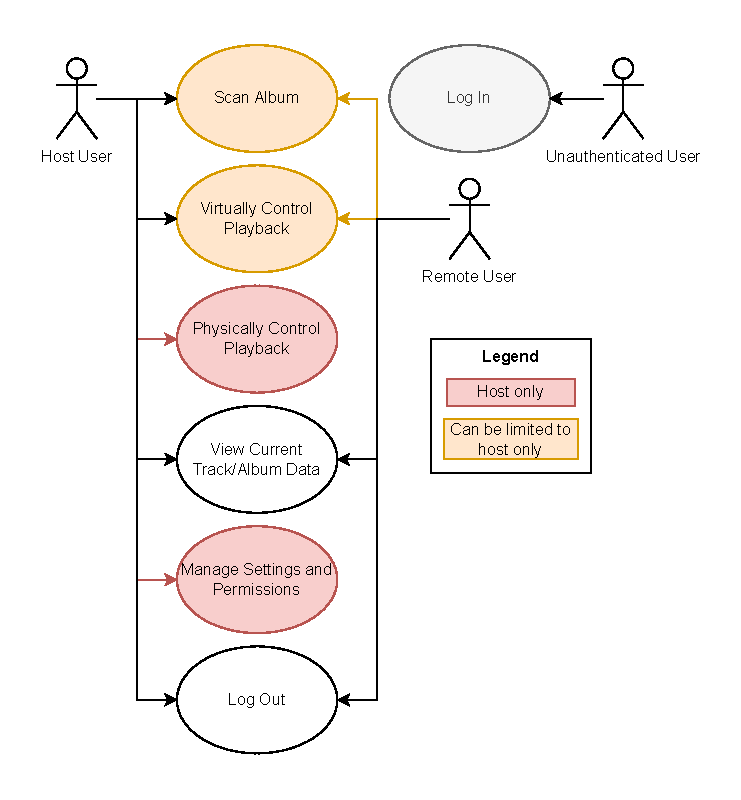
\includegraphics[width=0.65\linewidth]{images/UML_UseCase.pdf}
                \caption{A UML diagram of user use cases}
                \label{fig:umlusecase}
            \end{figure}
    
            \paragraph{Functional Requirements}
                \begin{itemize}
                    \item \textbf{FR1}: The system must identify album covers using image recognition with at least 90\% accuracy. This threshold balances feasibility and usability, ensuring reliable recognition without demanding unattainably high accuracy, based on similar machine-learning image recognition benchmarks (typical target: ≥85–90\%).
                    \item \textbf{FR2}: Album identification and music playback must start within 5 seconds. Five seconds represents a practical limit beyond which users begin to perceive the system as sluggish or non-responsive. This aligns with usability guidelines for interactive digital systems \cite{nngroupResponseTimes}.
                    \item \textbf{FR3}: The system must retrieve corresponding music tracks from Spotify after successful identification.
                    \item \textbf{FR4}: Users must be able to control playback (play, pause, skip) via software interface.
                    \item \textbf{FR5}: The UI must clearly display information about the album and track being played.
                    \item \textbf{FR6}: The interface must be intuitive and suitable for non-technical users.
                    \item \textbf{FR7}: The system must provide physical controls (buttons/dials) for basic playback operations.
                \end{itemize}
            
            \paragraph{Non-Functional Requirements}
                \begin{itemize}
                    \item \textbf{NFR1}: Total system latency (from recognition to playback) should not exceed 5 seconds.
                    \item \textbf{NFR2}: System reliability must ensure an operational uptime of at least 99\%. Ensures robust availability without requiring prohibitively expensive redundancy, aligning with standard reliability targets for consumer-oriented interactive systems
                    \item \textbf{NFR3}: Recognition failures should gracefully prompt user intervention without causing system crashes.
                    \item \textbf{NFR4}: The system must be fully compatible with Raspberry Pi 5 hardware.
                    \item \textbf{NFR5}: Setup and operation should be documented clearly, enabling ease of use without extensive technical expertise.
                    \item \textbf{NFR6}: The solution must adhere strictly to UK copyright laws.
                    \item \textbf{NFR7}: The system must comply fully with all used APIs' Terms of Services.
                \end{itemize}
            
            \paragraph{Constraints}
                \begin{itemize}
                    \item Implementation must accommodate the hardware limitations of chosen system (Raspberry Pi 5).
                    \item Use of API data must adhere strictly to their licensing and usage terms.
                    \item The dataset used for training image recognition must comply with UK legal guidelines for non-commercial research.
                \end{itemize}
            
            \paragraph{Assumptions}
                \begin{itemize}
                    \item Users have consistent and stable internet access.
                    \item Users possess active required accounts for playback services, where needed.
                    \item Operational lighting conditions are sufficient for accurate image recognition.
                \end{itemize}
    
        \subsection{Pillars of Design Philosophy}
    
            The following core principles were adopted in, and guided, the design phase:
    
            \begin{itemize}
                \item \textbf{Platform Agnosticism} The system was designed to avoid reliance on any single external component, using hexagonal architecture (plugs and adapters) to allow interchangeable parts, mandating components all conform to common interfaces. Flexibility extended across both services and device types, aiming to support a broad range of operating systems (OS) and hardware, emphasising the creation of a general solution.
            \end{itemize}
    
            \begin{itemize}
                \item \textbf{Physicality First} The device prioritises tactile interaction, echoing traditional vinyl players to maximise nostalgic appeal. Core playback controls must be usable fully with only the physical components; with digital enhancements remaining optional and unobtrusive.
            \end{itemize}
    
            \begin{itemize}
                \item \textbf{Digital Completeness} Every physical function is mirrored digitally to ensure full accessibility, particularly for users with impairments or lacking physical access. Though optional, the digital interface must integrate seamlessly; not to be treated as an after-thought.
            \end{itemize}
    
            \begin{itemize}
                \item \textbf{Open Source} With a firm belief in the importance and value of the open source community, the project will contribute, with all code being made public (subject to academic clearance), \footnote{Permission was granted to make the repository public on 13/03/25: \url{https://github.com/Razzula/virtual-turntable}} and all relevant aspects being clearly documented to maximise the usefulness of this project to others. Such tools and services were favoured where possible.
            \end{itemize}
    
            \begin{itemize}
                \item \textbf{Robustness and Maintainability} Emphasis was placed on clean, modular code using design patterns, single-responsibility principles, and comprehensive unit testing to ensure long-term reliability.
            \end{itemize}
    
            \begin{itemize}
                \item \textbf{Version Awareness} While the project was small enough to manage informally, care was taken to track changes in non-code elements such as schematics (Figures~\ref{fig:sketchPhys} and~\ref{fig:circuitDiagram}). This was recognised as an important practice for scalability -- large technical systems rely on advanced, formal PLM systems to manage such complexity (CERN)~\cite{friman2023plm}.
            \end{itemize}
    
            \begin{itemize}
                \item \textbf{Ethical Responsibility} The project was developed with ethical considerations at the forefront, accounting for copyright, transparency, responsible data use, and system security.
            \end{itemize}
        
        \subsection{System Architecture} % high-level system overview
    
            The final architecture design was to build a web application running on a single physical device, with both server and client hosted locally. Both physical analogue controls and exposed Representational State Transfer (REST) endpoints interface with the server, while the client handles audio playback and visual output. Communication between server and client occurs via both standard HTTP and bi-directional WebSocket channels, enabling real-time updates in both directions.
    
            The design incorporated a motor to spin a disc during playback, visually enhanced by matching visuals from the UI being vertically projected down onto the system, giving the appearance of a stylised vinyl with holographic overlays (e.g., current track information).
    
            Later in development, the architecture was extended to support remote clients. These external devices also connect via WebSockets, providing communal and accessible control, with the server updated to manage multiple concurrent connections (see Figure~\ref{fig:networkDiagram}).
        
            \subsubsection{Design Choices}
                % unique 1-1/1-many relation
                % server hardware control
                % host v. remote client
    
                \paragraph{Why use a web approach for a localised device?} Despite being local, a webstack aligned with streaming APIs and ensured device agnosticism. Its architecture also simplified later remote access expansion. Web technology also streamlined deployment without per-device setup and configuration being needed.
    
                \begin{figure}[h]
                    \centering
                    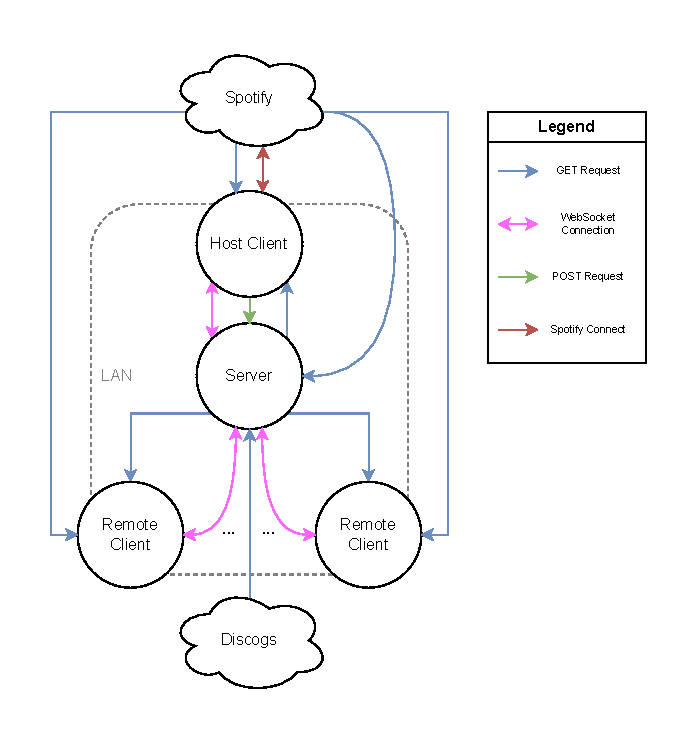
\includegraphics[width=0.75\textwidth]{images/VTT_network.NetworkDiagram.pdf}
                    \caption{Network diagram of system.}
                    \label{fig:networkDiagram}
                    \caption*{All requests between the host (client and server) and remote devices are over a LAN connection; with Discogs and Spotify being accessed externally over the web.}
                \end{figure}
        
            \subsubsection{System Stack}
    
                The system stack includes FastAPI\footnote{\url{https://fastapi.tiangolo.com/}}, React\footnote{\url{https://react.dev/learn}}, and RPi 5\footnote{\url{https://www.raspberrypi.com/products/raspberry-pi-5/}}; specific tools were chosen based on suitability for task and are detailed in the sections below.
    
    
        \subsection{Hardware}
    
            The system runs on an RPi 5, chosen for its flexibility, general OS support, and sufficient processing power for the lightweight CNNs used. Arduino boards were ruled out early, as their microcontroller architecture cannot support a full OS or run a web browser -- both essential for this project's web-based interface. The NVIDIA® Jetson Nano™\footnote{\url{https://developer.nvidia.com/embedded/jetson-nano}} was also considered, featuring an NVIDIA® Maxwell™ GPU with 128 CUDA® cores. In contrast, the Pi 5's VideoCore VII is designed exclusively for graphics and lacks support for general-purpose GPU compute like CUDA. While the Jetson offers superior acceleration, this was unnecessary given the model requirements -- and its higher cost, limited availability, and narrower versatility made it less suitable overall.
            
            Beyond functionality, aesthetics were key. To maximise nostalgia, the device used stylish mahogany wood with brass controls. Research shows that, in one survey, wood is the most frequently cited material in nostalgic household items, appearing in 34\% of nostalgic objects (with metal second at 21\%) \cite{Skinner2022}. These materials were ubiquitous in classic mid-20th-century audio equipment, so they instantly call to mind ``the charm of a bygone era'' \cite{LookInTheAttic2024}.
    
            \subsubsection{Hardware Components}
    
                It was essential to ensure all chosen hardware could be supported by the RPi 5's General-Purpose Input/Output (GPIO) pinout (see Figure~\ref{fig:RPi5Pinout}).
    
                \begin{figure}[htbp]
                    \centering
                    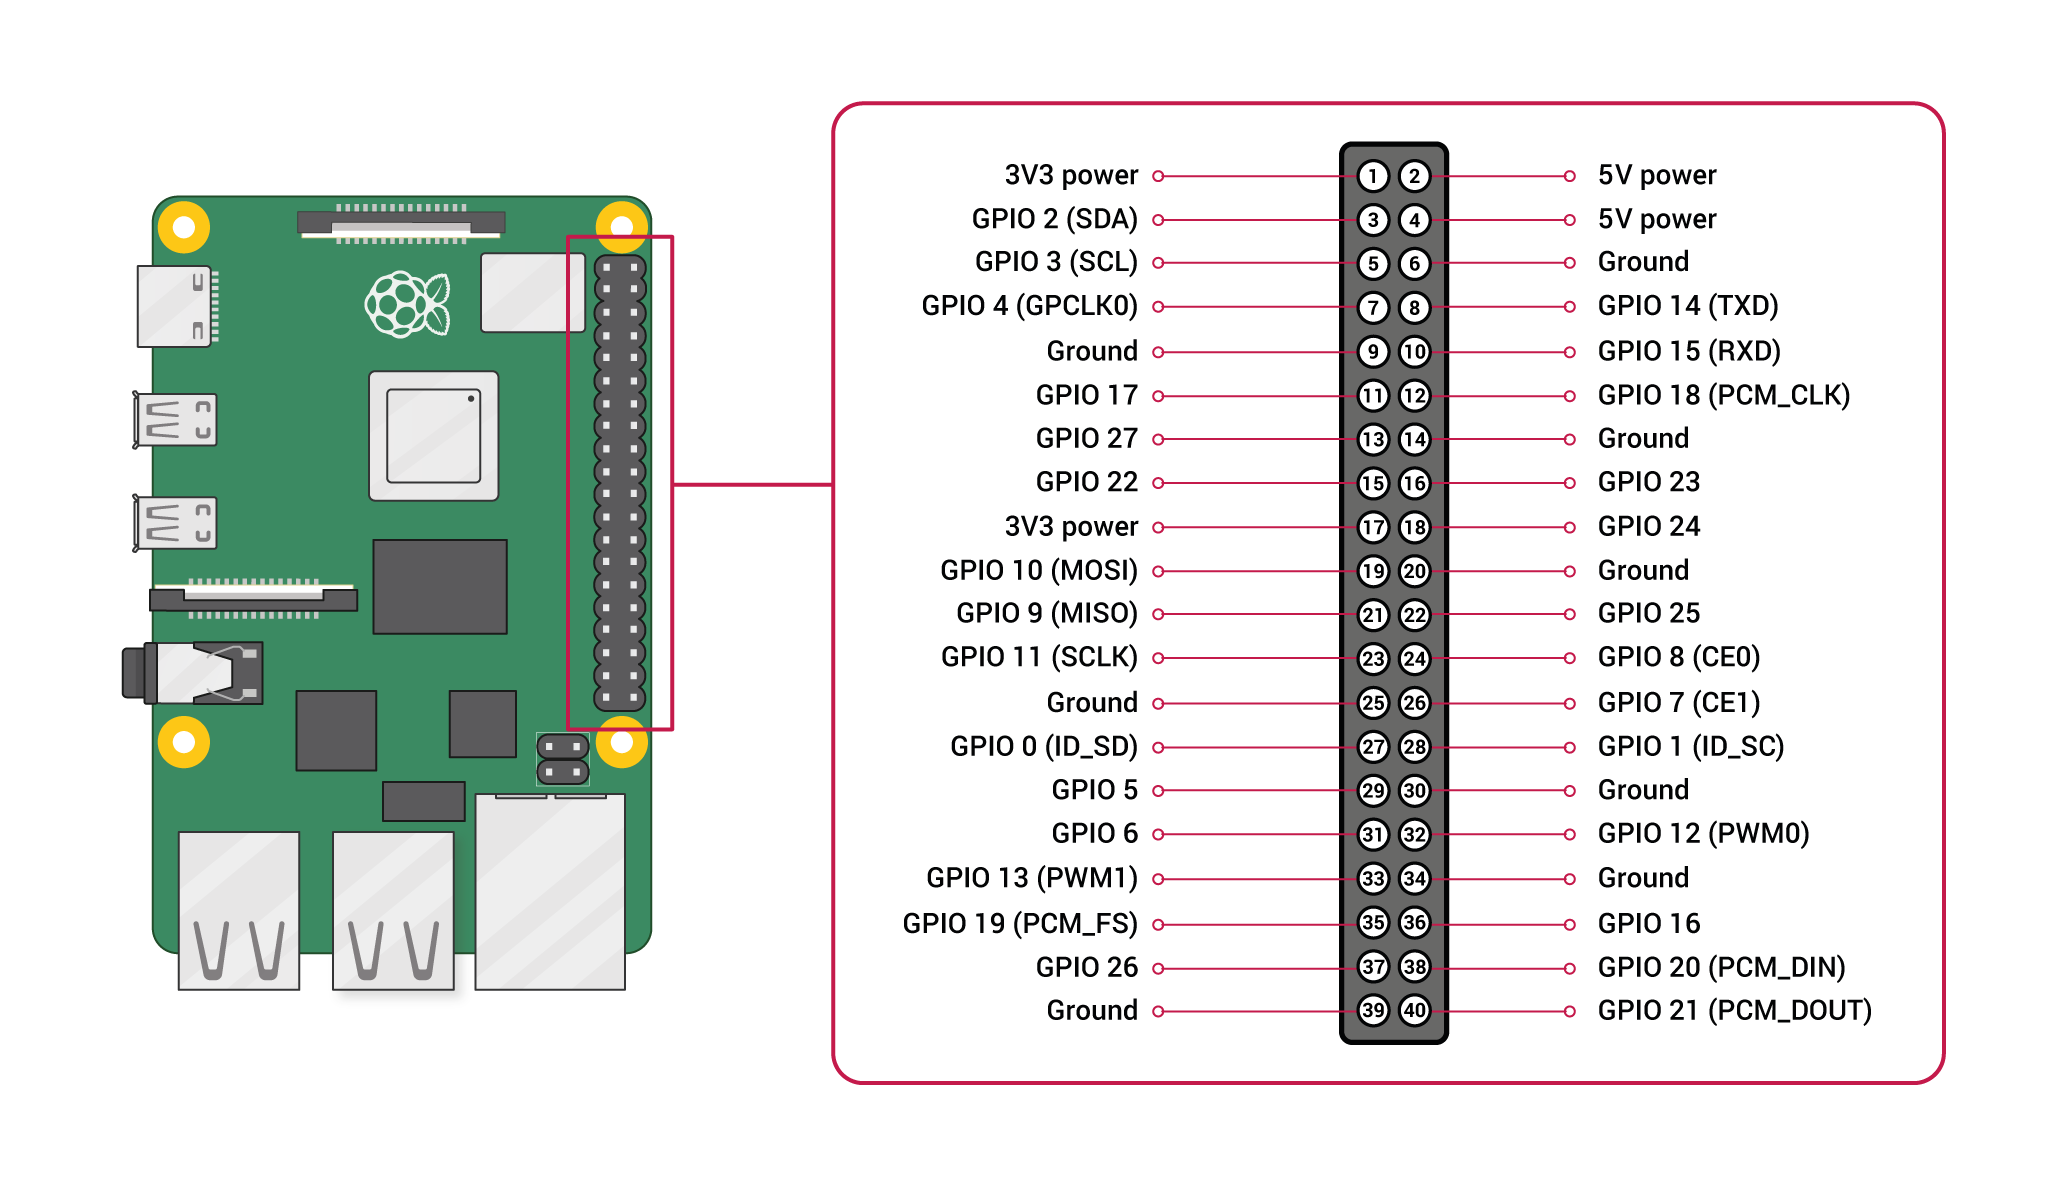
\includegraphics[width=\linewidth]{images/raspberry-pi-5-pinout.png}
                    \caption{Pinout configuration of Raspberry Pi 5}
                    \label{fig:RPi5Pinout}
                    \caption*{Sourced from \href{https://www.raspberrypi.com/documentation/computers/raspberry-pi.html#gpio}{Raspberry Pi Documentation} © 2012–2025 Raspberry Pi Ltd, used under CC BY-ND 4.0}
                \end{figure}
    
                Core components include a DC motor (via driver), rotary encoder switch, camera, and a trigger button (Table~\ref{tab:coreGPIOPins}). The rotary encoder supports vector input (with direction and magnitude) and button presses, enabling a compact control scheme:
    
                \begin{itemize}
                    \item \textbf{Knob rotation}: adjust volume.
                    \item \textbf{Button pressed, no rotation}: toggle pause/play.
                    \item \textbf{Knob rotation (button pressed)}: change to previous/next track, depending on direction.
                \end{itemize}
    
                \begin{table}[htbp]
                    \centering
                    \caption{GPIO Pin Requirements for Core Functionality}
                    \label{tab:coreGPIOPins}
                    \begin{tabular}{|l|l|l|}
                        \hline
                        \textbf{Component} & \textbf{Required Pins} & \textbf{Note}\\ \hline
                        \multirow{5}{*}{DC Motor (via Driver)} & 1 × 5\,V & Motor driver power \\ \cline{2-3}
                                                               & 1 × GND & Ground \\ \cline{2-3}
                                                               & 1 × 5\,V & Motor power \\ \cline{2-3}
                                                               & 2 × GPIO & Direction control (IN1, IN2) \\ \cline{2-3}
                                                               & 1 × GPIO (PWM) & Speed control (ENA) \\ \hline
                        \multirow{5}{*}{Rotary Encoder Switch} & 1 × 3.3\,V & \\ \cline{2-3}
                                                               & 2 × GPIO& Rotation data (CLK, DT)\\ \cline{2-3}
                                                               & 1 × GPIO & Button input (SW)\\ \cline{2-3}
                                                               & 1 × GND & \\ \hline
                        \multirow{2}{*}{Button (Camera Trigger)} & 1 × GPIO & \\ \cline{2-3}
                                                                 & 1 × GND & \\ \hline
                        Camera & 1 × USB or Ribbon Port & \\ \hline
                    \end{tabular}
                \end{table}
    
                Additional optional features included a hinged arm switch for playback control, offering a large, tactile alternative better suited for accessibility and immersion; a motor-mounted encoder for stall detection, preventing burn-out; and a second camera for scanning back covers (Table~\ref{tab:optionalGPIOPins}). These additions enhance safety, robustness, longevity, and engagement. While the dynamic knob offers fine control, its complexity may be a barrier -- mitigated by the simpler hinge mechanism, broadening interaction.
    
                \begin{table}[htbp]
                    \centering
                    \caption{GPIO Pin Requirements for Optional Components}
                    \label{tab:optionalGPIOPins}
                    \begin{tabular}{|l|l|l|}
                        \hline
                        \textbf{Component} & \textbf{Required Pins} & \textbf{Note}\\ \hline
                        \multirow{5}{*}{Rotary Encoder (Motor Stall Detection)} & 1 × 3.3\,V & Sensor power (VCC)\\ \cline{2-3}
                                                                                & 2 × GPIO & Rotation data (A, B) \\ \cline{2-3}
                                                                                & 1 × GND & \\ \hline
                        \multirow{2}{*}{Hinge Switch} & 1 × GPIO & \\ \cline{2-3}
                                                      & 1 × GND & \\ \hline
                        Secondary Camera & 1 × USB or Ribbon Port & \\ \hline
                    \end{tabular}
                \end{table}
    
                All components fit within the Pi 5's GPIO limits (Table~\ref{tab:pinSummary}), with a reasonable number of redundant pins to accommodate potential failures and room for expansions. However, all 5\,V pins are used; though, if needed, motor power can be offloaded to an external supply, which would free up one of these pins.
    
                \begin{table}[htbp]
                    \centering
                    \caption{Summary of GPIO and Port Requirements vs. Availability}
                    \label{tab:pinSummary}
                    \begin{tabular}{|l|c|c|c|c|}
                        \hline
                        \textbf{Pin / Port Type} & \textbf{Core}& \textbf{Optional}& \textbf{Total Required} & \textbf{Available} \textsuperscript{see Figure~\ref{fig:RPi5Pinout}
    }}\\ \hline
                        5\,V Power & 2 & & 2 & 2 \\ \hline
                        3.3\,V Power & 1 & & 1& 2 \\ \hline
                        GND & 3 & 2 & 5 & 8 \\ \hline
                        GPIO (Standard) & 6 & 3 & 9 & 28 \\ \hline
                        GPIO (PWM-capable) & 1 & & 1 & 4 \\ \hline
                        USB or Ribbon Port & 1 & 1 & 2 & 2+\textsuperscript{*}\\ \hline
                    \end{tabular}
                    \caption*{\textsuperscript{*}RPi 5 supports 4× USB + 2× camera ribbon ports.}
                \end{table}
    
                \begin{figure}[h]
                    \centering
                    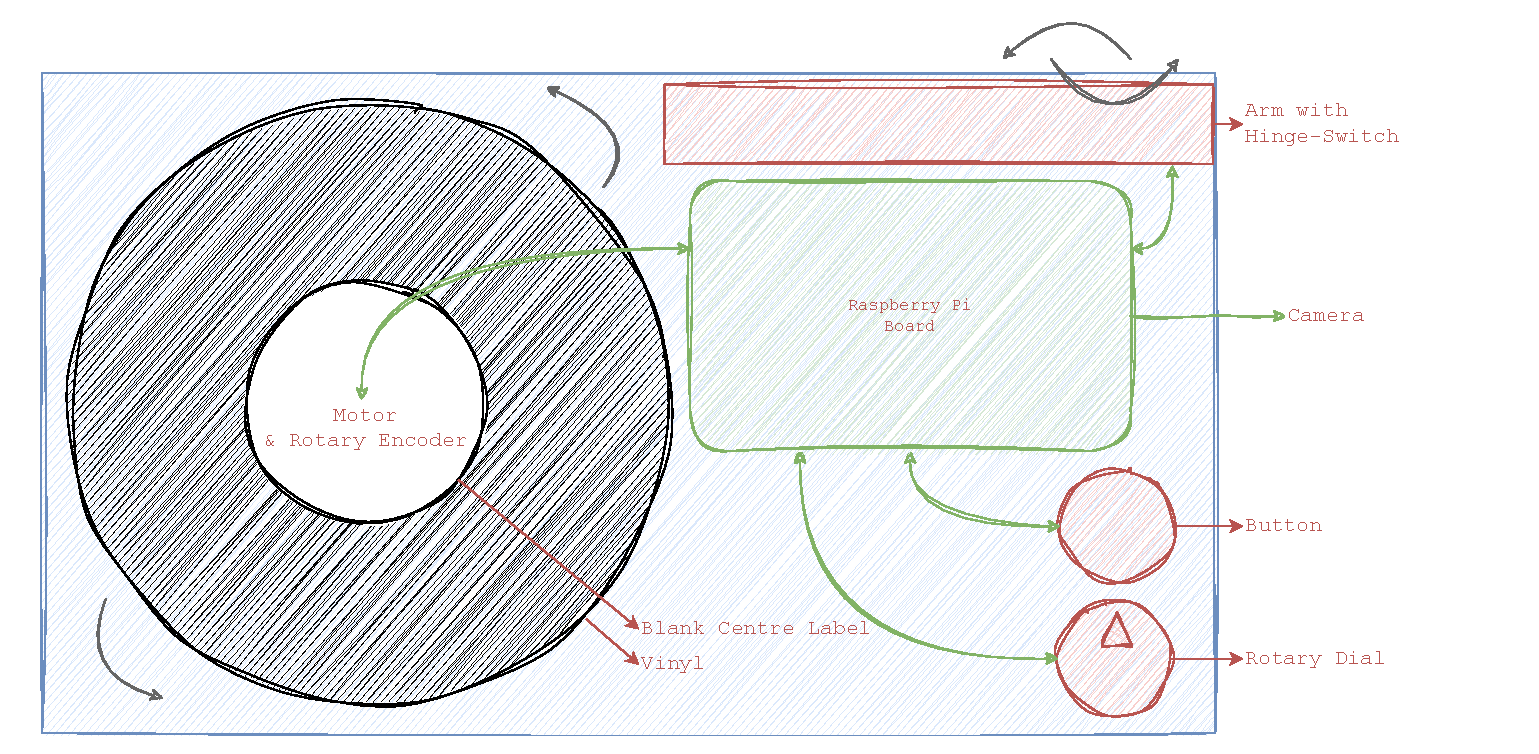
\includegraphics[width=0.95\linewidth]{images/SketchPhys.pdf}
                    \caption{Schematic layout of physical components and system wiring.}
                    \label{fig:sketchPhys}
                \end{figure}
    
            \subsubsection{Operating System}
    
                Raspberry Pi OS (or just RPiOS; formerly Raspbian), is an OS produced by the Raspberry Pi Foundation as the official OS for their chipboards. This makes interfacing with components such as GPIO pins seamless and easy. Although, in order to make the system as hardware-agnostic as possible, a standard Ubuntu kernel was used for the project. This forced solutions to not rely on native RPi interfaces, and so, whilst it made certain aspects more challenging, it means than the project is not locked to the RPi hardware.
    
                Ubuntu is also fully open-source, unlike RPiOS, which has some proprietary aspects. \footnote{RPiOS includes proprietary firmware and binary blobs required for booting and hardware functionality, such as the VideoCore GPU and wireless chipsets.}
    
    
                Firefox (also open-source) was used during development (as Ubuntu's default browser), with Chromium tested periodically to ensure cross-browser compatibility.
                
        
        \subsection{Front-end}
            \subsubsection{Primary User Interface}
                % lofi designs
    
                React was chosen for its strong support of reactive state updates from multiple sources -- crucial for the host client, which must synchronise state changes from its internal UI, external streaming vendor, and the server (see Figure~\ref{fig:statePropagationDiagram}). Prior experience with the framework was also an influence.
            
            \subsubsection{Audio Playback}
                % Spotify Playback SDK
                % Spotify Web API
    
                To maintain platform agnosticism, all streaming and metadata APIs are accessed through abstract interfaces, allowing seamless interchangeability. Spotify was chosen to be the streaming service for implementation due to prior experience, an existing subscription, and ease of integration with both front- and back-end components via its Web SDK\footnote{\url{https://developer.spotify.com/documentation/web-playback-sdk}}.
    
            \subsubsection{Minimal UI}
    
            Following the decision to build a single physical device, the UI was designed to be minimal and non-interactive by default -- entirely operable without a mouse, input, and screen. To emphasise physical-first design unobtrusively, Graphical User Interface (GUI) controls remain hidden unless the mouse was recently in motion, offering an easy fallback control. The UI mirrors the capabilities of physical controls and also further allows configuration of settings, including remote access permissions and motor toggling (available only for the host; see Section~\ref{sec:security}).
     
            \begin{figure}[h]
                \centering
                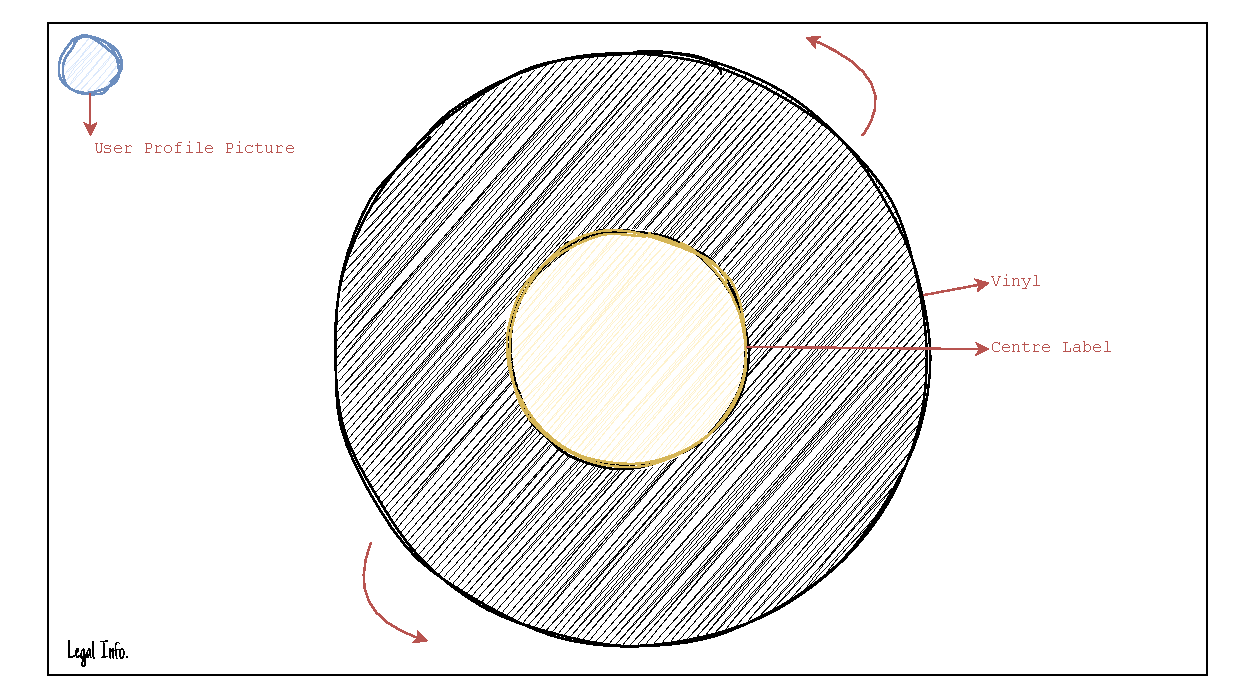
\includegraphics[width=0.85\linewidth]{images/SketchHostMin.pdf}
                \caption{UI wireframe of host client playing a track.}
                \label{fig:sketchHostQuiet}
            \end{figure}
            
            \begin{figure}[h]
                \centering
                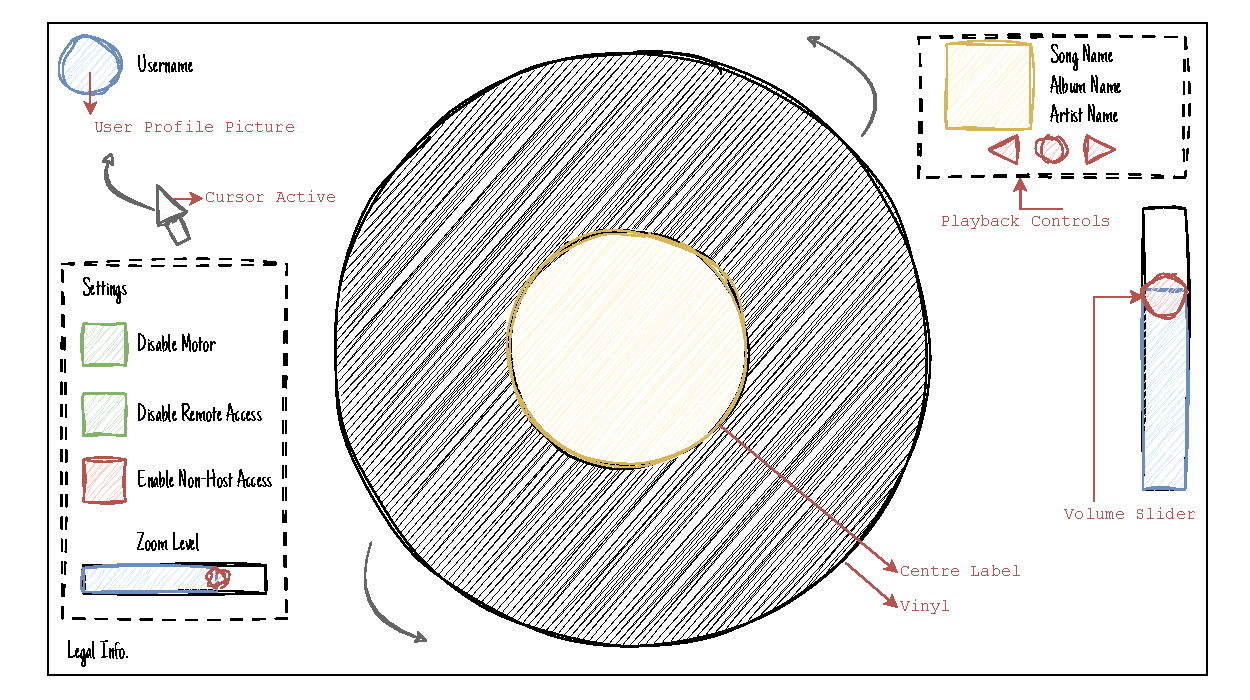
\includegraphics[width=0.85\linewidth]{images/SketchHostMax.pdf}
                \caption{UI wireframe of host client playing a track, with UI overlays.}
                \label{fig:sketchHostGui}
            \end{figure}
    
            It was important to ensure that the UI offered no less control and/or information as the physical controls did.
    
            Customisation of the UI was also an important aspect. As the physical device could vary between owners, user's should be able to set the proportions of the projection area, for example setting the baseplate's ratio, and the position and size of the disc. This would not only better accommodate different devices and setups (if the projector is closer, everything should be scalable to be smaller), but also allows creative expression for the user in letting them decide how to set up their system -- emphasised by even being able to disable the motor, if the user wants a quieter option.
        
            \subsubsection{Remote Clients}
    
                During development, the system was extended to support not only local browser access on the host device but also remote access from external devices such as mobile phones and computers. This decision was motivated by both accessibility and convenience. For users with physical impairments, remote access via phone allows full operation without needing to interact with hardware controls. It also enables users without required peripherals -- such as the camera -- to use their phone's camera for album scanning, instead of blocking it.
    
                Remote access further supports communal interaction: multiple users can simultaneously connect, control playback, or queue music, creating a shared experience. It also preserves some degree of portability from the original mobile concept -- users can scan an album when away, and upload it to the system when they are next connected, instead of relying solely on real-time images from cameras.
                
                Rather than implement a separate front-end or routing system, the client was implemented as a single-page application, with the UI adapting based on whether the device is the host or remote, determined via a server query. This also maximised component re-usability, to help ensure the system was robust without major additional testing being required.
    
                \begin{figure}[h]
                    \centering
                    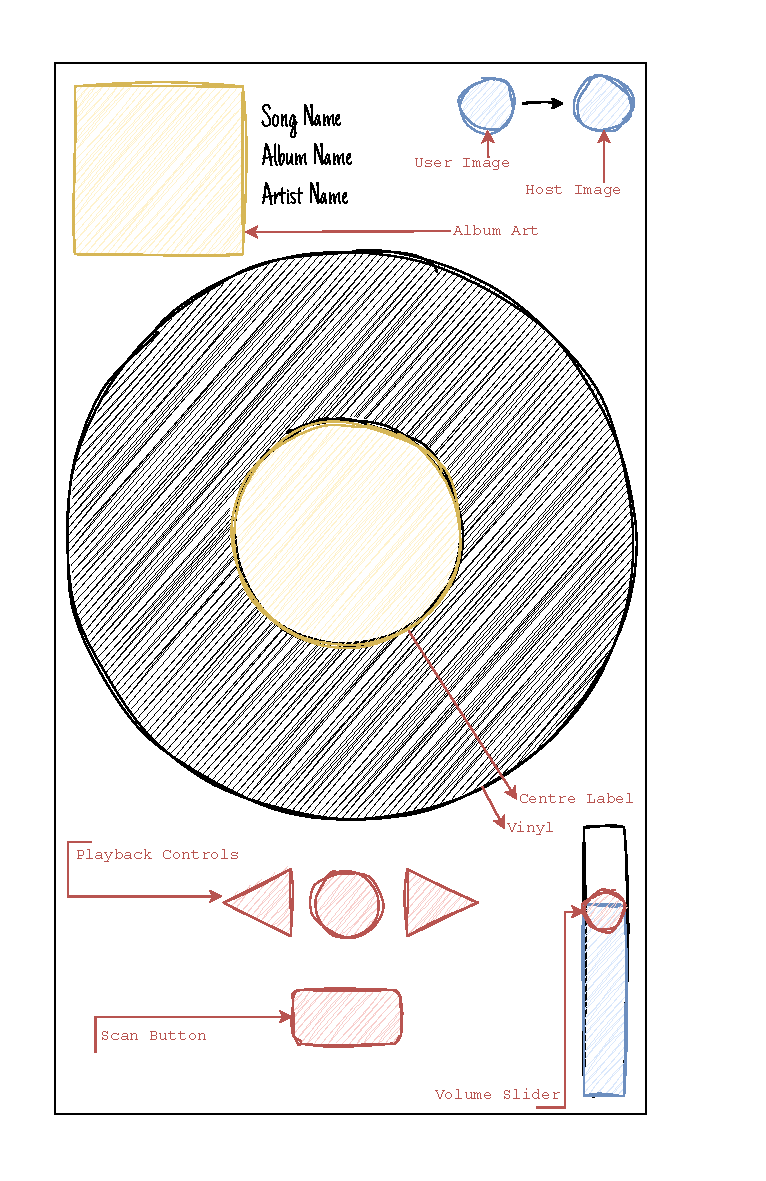
\includegraphics[width=0.55\linewidth]{images/SketchRemote.pdf}
                    \caption{UI wireframe of remote client (mobile).}
                    \label{fig:sketchRemote}
                \end{figure}
                
                The remote interface mirrors the physical controls' functionalities, offering playback (play, pause, skip, previous), volume adjustment, album scanning, and even access to the host's owned album library, which can be browsed or shuffled. Remote users can perform any action available to those physically interacting with the device.
    
        
        \subsection{Back-end}
    
            A centralised server was required to coordinate communication between multiple clients, handle physical controls, run album detection (see Section~\ref{sec:mlDesign}), manage authentication (see Section~\ref{sec:security}), and orchestrate system logic.
    
            Python was chosen for its simplicity and strong ML ecosystem. FastAPI, with Uvicorn, \footnote{\url{https://www.uvicorn.org/}} was selected as a lightweight, async-friendly framework suitable for the Pi.
    
            The server uses the singleton pattern to ensure the ML model loads only once. While scalability wasn't a primary concern, following this and the Single Responsibility Principle (SRP) ensured a modular, maintainable codebase -- e.g., separating API routes, authentication logic, and control systems into distinct classes.
    
            As the server handles both physical controls and remote commands (see Figure~\ref{fig:statePropagationDiagram}), real-time, bi-directional communication with clients was essential. WebSockets were chosen over inefficient polling techniques or Server-Sent Events (SSEs) for their low-latency, duplex nature, allowing consistent synchronisation whether updates originate from the server (e.g., physical input) or the client (e.g., remote Spotify actions). This unified channel avoids duplicating logic across multiple communication methods (such as identical handlers for both REST and SSE pings).
        
            \subsubsection{Metadata Retrieval}
                % Discogs API
                % assert Discogs ToS compliance (not used for AI)
    
                Traditionally, when a track or album is playing, online streaming services show the cover art to the user. Since this project relies on scanning a cover art in order to play the music, it seemed redundant to broadcast the current track by showing the user the same artwork they have in their hands. So, rather than duplicating this, and in order to lean more into the physical vinyl concept, the server was designed to fetch the centre label of the corresponding vinyl, in order to show this on the disc, instead.
    
                In order to fetch this, Discogs' API\footnote{\url{https://www.discogs.com/developers}} was used, as they maintain a carefully curated library of many images for vinyls, including high-quality images of these labels. Whilst Discogs do not allow their images to be used in AI systems, they can be used if strictly processed by traditional computer vision (CV) methods. Using Hough Circle detection, the image library of the relevant album can be scanned for the best-fitting circle, which, then cropped, can be served to the front-end.
          
        \subsection{Machine Learning Model Design} \label{sec:mlDesign}
    
            Based on the background research, a machine-learning approach was chosen over tailored OCR or feature extraction methods, as album covers can often lack text and vary widely in design. While visual transformers have the best performance on large datasets, a smaller CNN was selected to better converge on the more limited and specific dataset of albums used here.
        
            \subsubsection{Dataset Collection}
                % use of CoverArtArchive
    
                A suitable dataset was required for training. Manual image collection would be slow and risk bias, and most services (e.g., Spotify, Discogs) prohibit using their assets in AI systems. \textit{Last.fm}'s \footnote{\url{https://www.last.fm/api}} terms posed no explicit restrictions, but the \textit{Cover Art Archive} \footnote{\url{https://coverartarchive.org/}} (via the \textit{Internet Archive} and \textit{Musicbrainz}) was selected due to its open licensing in addition to the inclusion of images of the backs of covers -- something other platforms lacked.
    
                To ensure unbiased validation, manually photographed images were still collected separately, though to a limited extent due to physical availability constraints (see~\ref{data:val}).
    
            \subsubsection{Solution Design}
    
                The core aim was to classify scanned album covers using a CNN. To detect cases where no album is present (e.g., the camera triggers too early), a ‘null' class of random images was included. These would be carefully curated to avoid distorting the classifier's behaviour. However, since the system runs on a single, static device, the camera's background is expected to remain stable -- allowing this null class to instead reflect the actual backdrop seen when no album is present.
    
                This stability could be further leveraged using temporal background subtraction: averaging multiple frames over time to generate a `baseline' image. Subtracting this from new frames would help detect the presence or absence of an album, and also prevent the background influencing predictions (e.g., small albums revealing too much background).
    
                If null classification worked well, the camera could continuously poll images and automatically react when a new album is detected -- removing the need for manual input. That said, this would be an optional accessibility feature, as the physical act of taking a photo was seen as an important, engaging element.
    
                To further improve robustness, the system should not rely solely on the CNN. When classification confidence is low, it could fall back on OCR and barcode scanning to inform or resolve the decision. This combinatorial approach would help manage edge cases and albums not represented in the training data. Confidence thresholds should be tuned experimentally. Additionally, the model could be extended to support more advanced classifications or enhanced using Reinforcement Learning (RL), as illustrated in Figure~\ref{fig:classifyFlowchart}.
    
                \begin{figure}
                    \centering
                    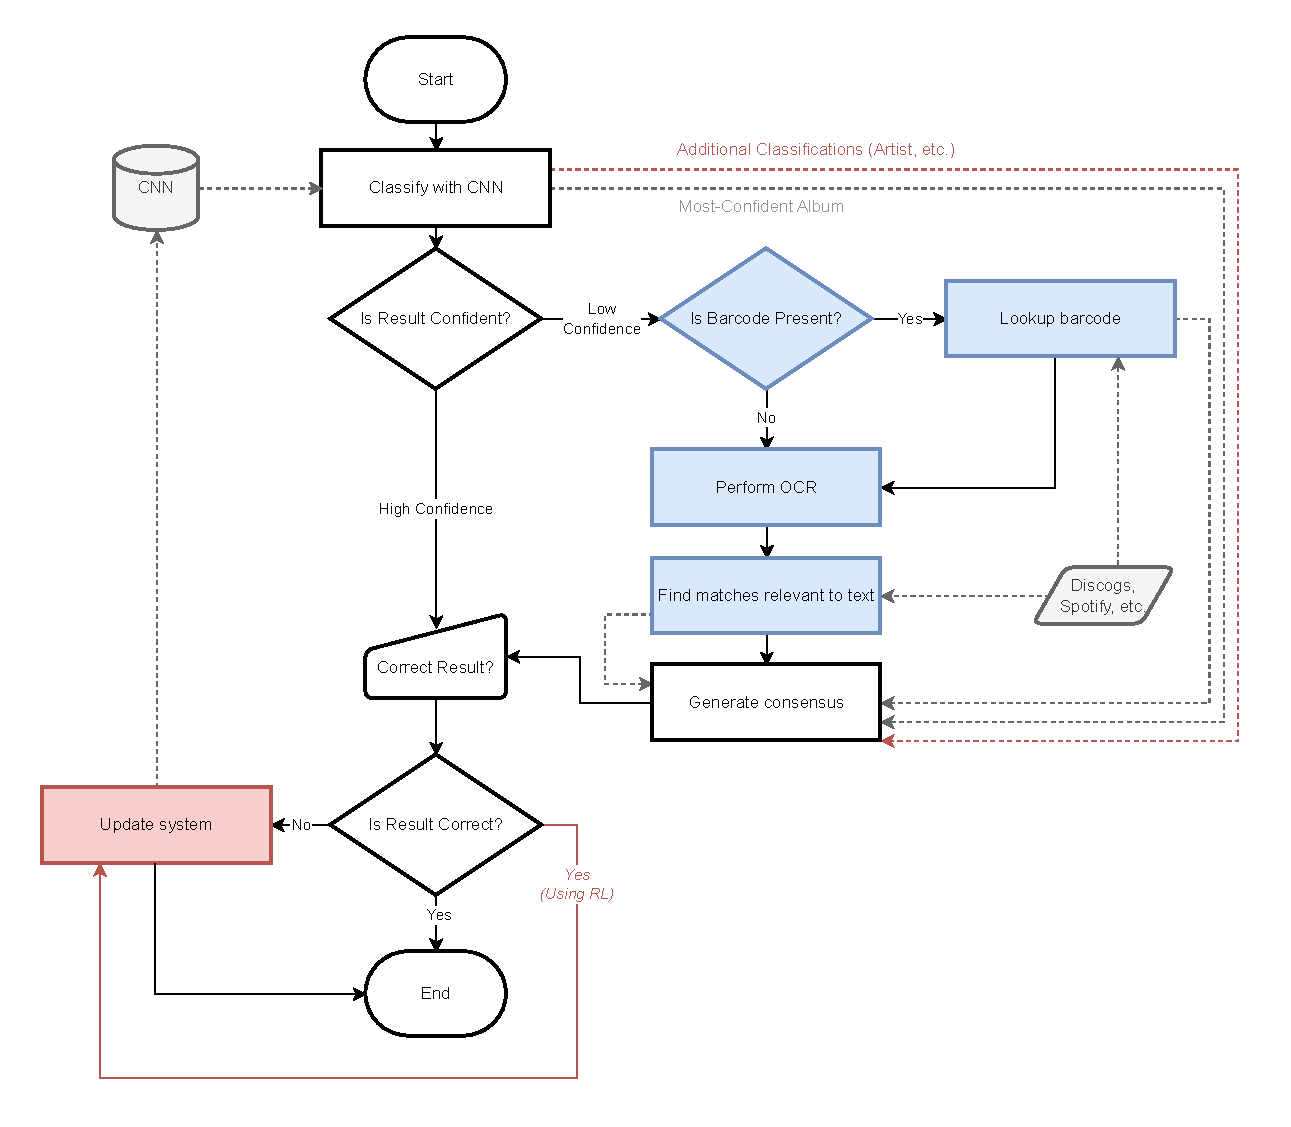
\includegraphics[width=0.85\linewidth]{images/ClassifyFlowchart.pdf}
                    \caption{Decision Flowchart for Image Recognition}
                    \label{fig:classifyFlowchart}
                    \caption*{Blue elements indicate fallback mechanisms; red highlights aspirational features.}
                \end{figure}
        
            \subsubsection{Model Architecture}
    
                A CNN was used for its proven ability in image classification. The design followed an educational, iterative approach: starting with a minimal model, then incrementally expanding and tuning it based on performance.
                
                Model architecture was developed incrementally during implementation, guided by experimental results rather than predefined designs. The details of each of these models is described in Section~\ref{sec:mlImp}.
    
                In order to distinguish the models conceptually, each was named after a snake-like creature from Greek mythology (see Appendix~\ref{app:Greek}).
    
                \paragraph{Ouroboros} A standard feed-forward CNN, designed for closed-world classification of known album artwork.
    
                At this most basic level, the goal is to simply design a model that can accurately learn information from both a small and large dataset of albums, to ensure that it can handle varying collection sizes of different users.
    
                Since album artworks rarely vary between copies, the task is effectively a closed-world classification problem. The model can therefore prioritise memorisation over generalisation moreso than a standard model. This memorisation-friendly nature inspired the name Ouroboros -- referencing the Greek self-consuming serpent (see Appendix~\ref{app:Greek}).
    
                \paragraph{Amphisbaena} A dual-headed\footnote{Refer to Appendix~\ref{app:Greek} for details on the two-headed Amphisbaena serpent.} neural network, trained to capture and classify an image's most likely artist, in addition to the album itself.
    
                Building on Ouroboros, a dual-headed model was explored to predict both album and artist.
    
                If the album was unseen, it could never be predicted, yet, by predicting an artist, with high confidence, where no album is overly confident: this could be used to inform and guide the fallback system by limiting search scope to said artist.
    
                Additionally, through further experimentation, this could be expanded to learn genre, or even the decade of release.
    
                \paragraph{Hydra} An expandable architecture supporting the addition of new classes\footnote{Hence the name, inspired by the Greek Hydra of Lerna (see Appendix~\ref{app:Greek}).} without retraining the entire model.
                
                % An adaptive multi-headed model, allowing the creation of new heads through knowledge distillation and consensus to learn new, previously out-of-scope classes, whilst still maintaining precision on previously trained data.
    
                A key limitation of closed classification is that it cannot predict classes outside the training dataset. Whilst it is common practice to re-train (or fine-tune) a model, to adjust weightings based off of new data, the task of adding a whole new class to the model's options when deciding is a much more complex task.
    
                The simplest option is to re-train the whole model, with the original and additional classes and data. But, in order to best maintain legal fair dealings, all images used in training were deleted after use. Re-downloading the dataset each time would be impractical, especially as some images may later be removed from the source, potentially degrading model performance if retrained.
    
                An aspiration target of model development for this project was to create a progressive neural network (PNN) that could adapt to new classes. The goal was to support dynamic class expansion by training new heads as needed. Each new head would use knowledge distillation from previous ones to avoid forgetting prior classes. Predictions would then be made through a weighted consensus across all heads.
    
        \subsection{Security Considerations} \label{sec:security}
            % handling of auth tokens (transient)
            % off-handing of persistence tasks
            % network hosting
            % option of same-user or any-user controls
            % API compliances
            
            Though the system is designed as a local device, with connectivity only to trusted APIs, security was treated as a critical consideration at every stage.
    
            \paragraph{Secure Data Handling} The system uses a standard RESTful token flow. After a user authenticates via an external service, the returned token is stored in memory and linked to their session cookie. Only the originating device can access this token, ensuring isolation and secure access.
    
            The exchange of data between components is illustrated in Figure~\ref{fig:security}. From this, critical and important elements -- such as API keys, tokens, and control commands -- were identified and highlighted. These are handled with particular care, as compromising them would risk exposing the service and other devices. Image uploads were also marked as an area of concern. Although not designed for sensitive content, the system takes a precautionary approach: images are deleted after use to reduce risk and avoid potential negligence.
    
            \paragraph{Delegated Persistence} Where possible, non-sensitive user data (e.g., scanned album lists) is stored using external APIs. For example, Spotify playlists are used as persistent storage, shifting GDPR compliance responsibilities to the vendor.
    
            \paragraph{Local Network Access} To support remote control, \textit{Vite's} \footnote{\url{https://vitejs.dev/guide/}} network-hosting allows LAN devices to connect. As the system is intended for home use, this is considered safe, provided firewall protections are in place.
    
            \begin{figure}
                \centering
                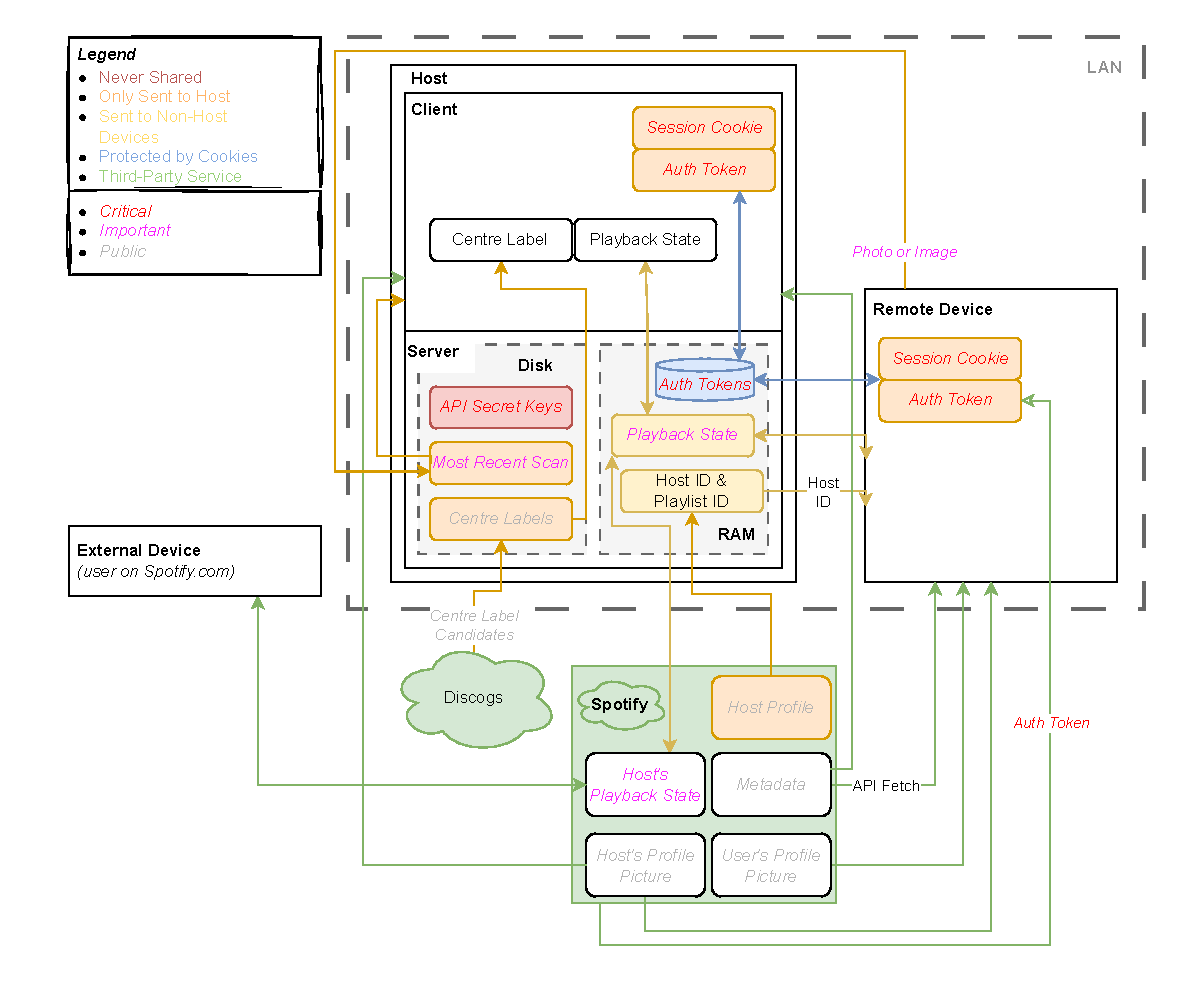
\includegraphics[width=0.95\linewidth]{images/SecurityDiagram.pdf}
                \caption{Security Architecture Diagram}
                \label{fig:security}
                \caption*{Some connections are trimmed or excluded for brevity-- greater granularity can be found in Figure~\ref{fig:statePropagationDiagram}.}
            \end{figure}
    
            \paragraph{Command Permissions} Remote control is restricted based on user permissions, configured by the host. Permissions are validated server-side using session cookies and external token verification to prevent unauthorised control.
    
            \paragraph{API Compliance} All integrations comply fully with the relevant API terms of service, including rate limits and usage restrictions.
        
        \subsection{Testing Methodology}
            
            \subsubsection{Validation of Effectiveness}
    
                Three metrics evaluate effectiveness:
    
                \paragraph{Model Performance} Model performance will be evaluated formally using two components: the recognition model and metadata retrieval. A separate test set (\ref{data:trueTest}) of front-only physical cover photos will be used to compute an F1 score -- the harmonic mean of precision and recall -- which balances false positives and false negatives. Additionally, the centre label accuracy can be objectively assessed by running it over a known set of albums and manually verifying label accuracy against the owned vinyls.
    
                \paragraph{Usability} An important goal is whether or not the system and its physical and digital controls are accessible and useful for users. To assess this, a user-centric approach will be taken, with evaluation of survey results\footnote{The evaluation form is accessible at \href{https://forms.gle/DS8oik9Vyny6Zxnk6}{https://forms.gle/DS8oik9Vyny6Zxnk6}} of people who have used the finished system.
    
                \paragraph{Code Robustness} To ensure functional and robust code, a comprehensive unit test suite will be developed in parallel. Development was not test-driven, in order to preserve flexibility during experimental design. This suite will aim for high code coverage.
        
            \subsubsection{Validation of Affectiveness}
                
                In addition to the practical side, the emotional value of the system also needs assessment. In order to ensure that the system has correctly appealed to its intended audience and to evaluate how well it balances vinyl appeal and digital convenience, the user survey will also include questions regarding these aspects. These questions aim to determine whether the system captures the nostalgic appeal of vinyl while providing the practical benefits of modern systems.
    
    %%%%%%%%%%%%%%%%%% SECTION 4 %%%%%%%%%%%%%%%%%%
    \section{Implementation}
        % details realised in practice
        % challenges, and how overcame
        % code-level or system-specific decisions, optimizations, or trade-offs
        % integration
    
        During development, several changes and refinements were made in response to practical challenges and emerging opportunities. While the original design served as a strong blueprint, some technical and hardware constraints necessitated creative problem-solving and re-evaluation of certain assumptions.
    
        This section describes the practical implementation of the frontend, backend, hardware, and ML components. It highlights key deviations from the design, integration details, and specific trade-offs made during the build process.
    
        \subsection{Front-end}
    
    
            The implementation of the front-end system was relatively smooth, largely due to the minimal-UI aspect of the design. The interface was designed to be practical first, with little-to-no creativity or flair being added until late in development.
    
            Once functional, polish was added. For example, when an image is taken/uploaded to the system, it is briefly displayed on the screen before being `lifted up' to unveil the vinyl and its centre label underneath.\footnote{A video demonstration of this is available at \url{https://youtu.be/t4fFDltrNjo?si=KGCiWdh4BDu7QLDN&t=189}.}
    
            \subsubsection{Frontend Personalisation and Audio Effects}
    
            An alternate local audio player was developed alongside Spotify integration, enabling playback of user-stored files. This addressed notable gaps in Spotify's catalogue -- particularly rare or compilation vinyls -- and also allowed the system to function in an offline setting, independent of internet connectivity.
    
            To enhance the user experience and evoke the character of physical media, a feature was introduced to overlay randomised noise and static onto locally played tracks. This added perceived `warmth', associated with vinyl playback, offering a more personalised and nostalgic feel across different devices.
            
            Due to Spotify's Developer Terms \cite{spotifyDevTerms}, such modifications could not be applied to streamed content, as altering or layering audio over Spotify's output is strictly prohibited. However, for locally stored files, no such restrictions applied.
            
            As a basic proof of concept, a static noise layer was generated and played throughout the track, with subtle fluctuations in volume. The noise profile was determined using a hashed seed based on track metadata and playback time, ensuring variation across devices and tracks, while maintaining consistency for repeated plays by the same user. This meant that even the same audio file would sound slightly different depending on the user and device. The concept could be extended to introduce additional artefacts -- such as scratches, pops, or pitch modulation -- to more closely emulate the idiosyncrasies of vinyl.
    
            Much later into the project's lifecycle, when testing and evaluating the product, it was realised that a nail could be mounted onto the `arm' switch to better visually mimic a record player's needle. This even further improved the likeness beyond just the visual, as the nail scraping along the disc's surface created a scraping noise\footnote{This can be heard at \url{https://youtu.be/t4fFDltrNjo?si=WsohmFwt4dQPNFcC&t=110}.} -- unique to the user's nail and grooves on the vinyl being used a projector surface -- without violating Spotify's terms of not overlaying other sounds.\footnote{Appendix~\ref{sec:nailArt} explores some tangential thoughts on the final result of using this solution.}
        
            \subsubsection{Challenges Encountered}
    
                \paragraph{Responsiveness vs. Wholeness} During development one challenge that was encountered was the latency that would sometimes occur in fetching a track's metadata after the track had started playing. In order to give the user as seamless of an auditory experience as possible, it was best to let tracks play instantly, with no delay. However, this meant that sometimes the centre label would be blank briefly before `popping in' afterwards. Generally, UI principles dictate that an aspect should be loaded in completeness before rendering, to avoid unstable changes being displayed to the user. Since the system is primarily an audio system, it was decided to favour responsiveness, allowing the system to asynchronously update the interface if and when it got the metadata. In order to mitigate the pop-in, once a centre label is found the image was cached in the file-store, to prevent this search process being conducted each time. Furthermore, the aforementioned image display covering the vinyl, gives more of a chance for the pop-in to be hidden from the user, for those few seconds.
    
                \paragraph{DRM Issues} One notable issue came from the choice of the system's hardware. Raspberry Pi Single-Board Computers (SBCs) use ARM-based processors. Whilst Ubuntu supports this, a notable absence is that Google's WideVine Digital Rights Management (DRM) (which is used by both Firefox and chromium-browsers alike) does not have an official AArch64 build, which is needed for a RPi. The absence of a DRM meant that Spotify's audio could not be streamed in the browser. Whilst no AArch64 build exists in the official repos, there is an official build used for ChromeOS systems. It was possible to install and use this version, which enabled DRM content on the Pi. Without it, this would have been a serious hurdle for the project's chosen system architecture.
    
                Additionally, there were some issues with missing media codecs in Ubuntu's default packages. This was easy to resolve, at the cost of adding more steps to the setup process, which required a greater need for documentation. This would have been minimised if using more established solutions, such the official Raspbian image on the Pi, or a proprietary OS such as Windows on an x64 board.
    
            \subsubsection*{Reflection}
                The minimal-UI approach streamlined implementation and fit the aesthetic aims, but surfaced UX quirks like unclear hidden controls. DRM limitations on ARM were an unexpected hurdle -- thankfully overcome -- but highlight a fragility in relying on vendor ecosystems.
    
        \subsection{Back-end} % maybe Front/Back should just merge to software, here
    
            The backend was developed with Python's FastAPI and asyncio libraries to maximise the performance of parallel tasks. In addition to this, PyTorch (see Section~\ref{sec:mlImp}) and OpenCV\footnote{\url{https://docs.opencv.org/}} were used to make the machine learning and image extraction processes simpler to perform.
    
            \paragraph{State Management}
            One interesting feature of the system, was that a state-propagation system essentially had to be created. Since the system can be split into three components (host client, remote client, and server), which also integrate with external systems (such as Spotify), all of these components had their own internal state which informed the system how to act, but needed to be writeable from the other components. The solution to this was to essentially create a reactive system, inspired by React's state and hooks system. All active components are linked in a linear chain (see Figure~\ref{fig:statePropagationDiagram}), therefore, other components states can be seen as dependencies. Each component is only concerned with updating adjacent components, when its internal state changes. Whenever a state changes, it is broadcast to connected neighbours. This creates a real-time feedback loop, allowing changes, even from an external device using the official Spotify app, for example, to be synchronised with the motor's state. For each aspect, a single `point of truth' was determined, and in cases where new connection are established, this was used. For example, the audio is playing through the host client app, and so, if there is a conflict of states, the host client's state is favoured.
            
            \begin{figure}[h]
                \centering
                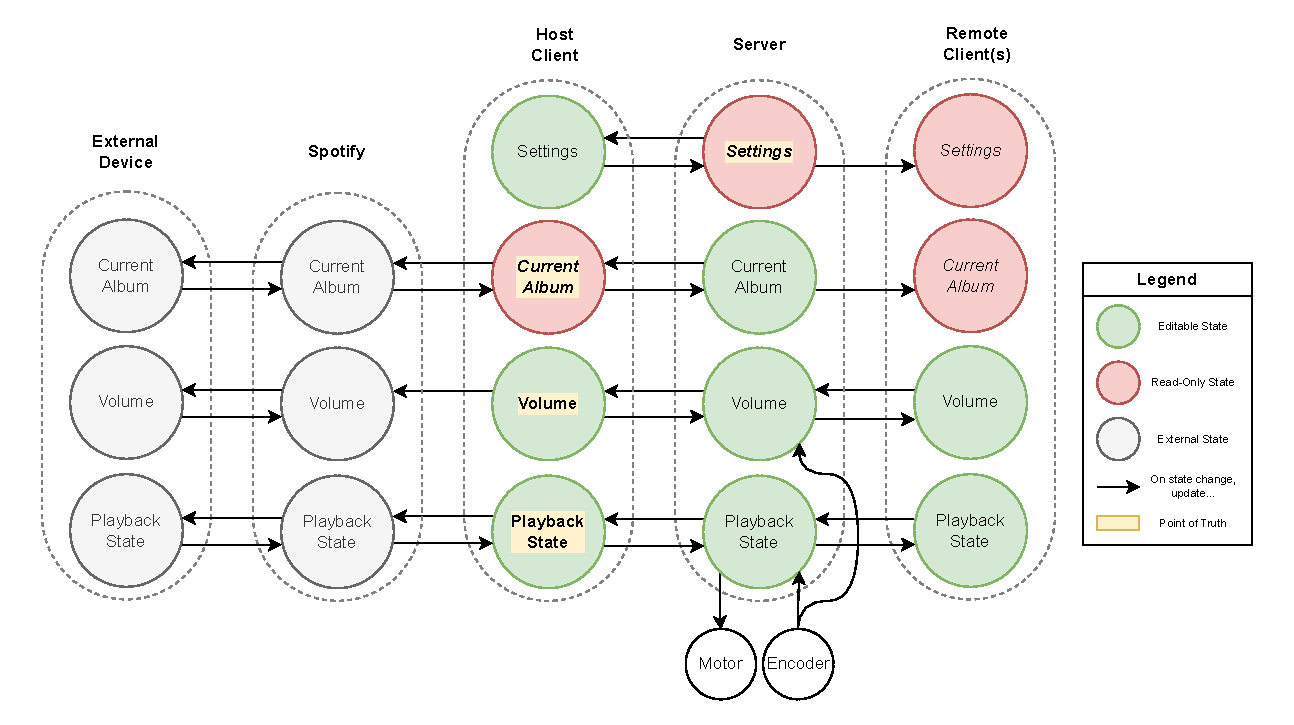
\includegraphics[width=\textwidth]{images/VTT_states.DependencyGraph.pdf}
                \caption{Dependency diagram showing state propagation model between both system and external components, allowing real-time reactivity to state changes from multiple sources.}
                \label{fig:statePropagationDiagram}
            \end{figure}
    
            One complication of this feature, was that there were often superfluous broadcasts. For example, if component A updated component B, then it is wasteful for component B to broadcast that same change back to component A. However, most of these broadcasts were kept, as it essentially created a `handshake' system where components were not only updating each other, but received confirmation that those updates had been performed. The exception to this was in the front-end clients, where external and internal changes were flagged, to ensure that only internal changes were broadcasted. This was important because React's state system already handles state tracking, and could cause infinite feedback loops, throttling performance and the system's communication bandwidth. Additionally, since the host client interfaced directly with external components, it was best to avoid `spamming' these components, which could result in timeouts.
    
            \paragraph{Alternate Processes}
    
            An important consideration was supporting multiple triggers for the same process -- for instance, initiating album detection and playback via either a physical camera button or image upload from a remote device (see Figure~\ref{fig:imageSequenceDiagram}).
    
            \begin{figure}[h]
                \centering
                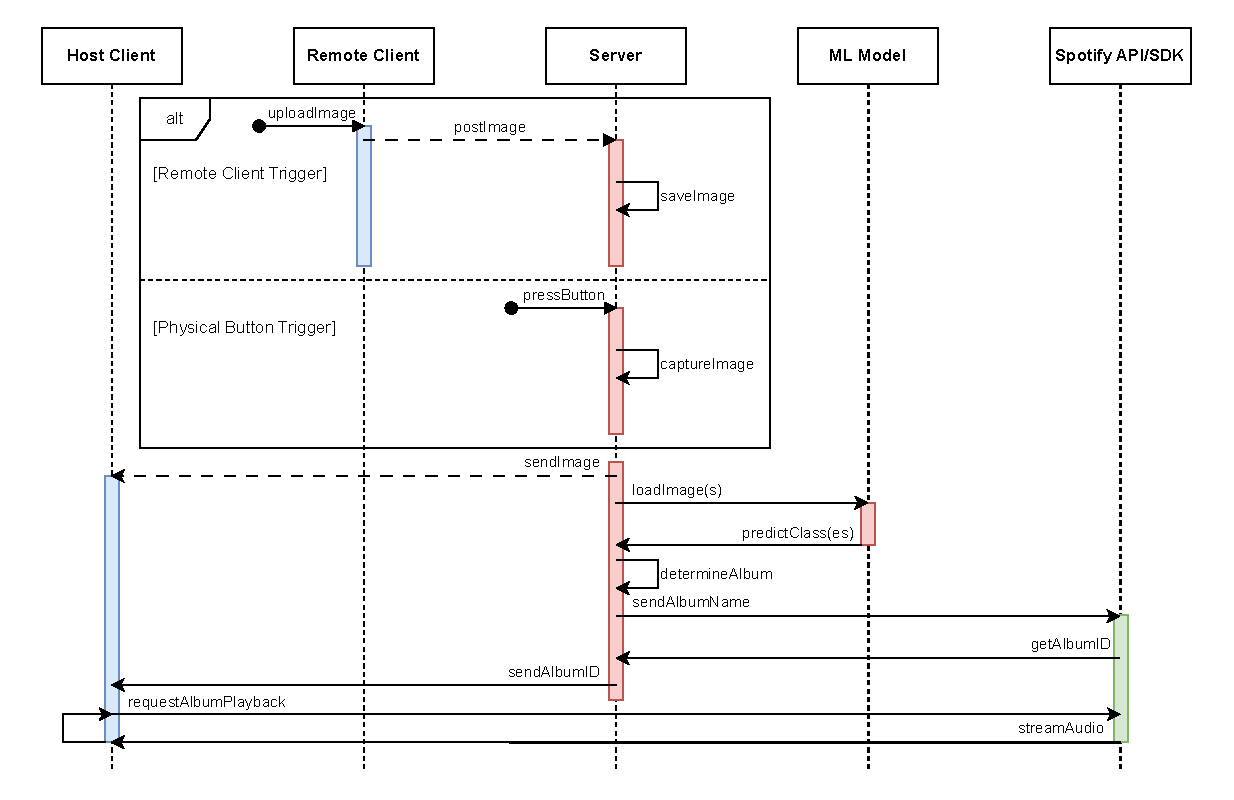
\includegraphics[width=\textwidth]{images/VTT_imageScan.SequenceDiagram.pdf}
                \caption{Sequence diagram showing two alternative triggers (client upload and server capture) leading to image processing and metadata retrieval before sending playback instructions to the host.}
                \label{fig:imageSequenceDiagram}
            \end{figure}
    
            In order to maximise the code's maintainability, re-using the code for the shared part of the process was of utmost importance, however since one trigger was an asynchronous REST endpoint, and the other a low-level polling of hardware. This would have been very difficult to manage if these functions were not in isolated components. Keeping with SRP practices, as decided early on, prior to any development, helped accommodate these mid-implementation changes to the system, with minimal complications.
    
            \paragraph{Metadata Retrieval}
    
            When fetching the centre labels from Discogs, using a simply query generated from the Spotify metadata, the images are downloaded and analysed one-by-one, aiming to find a one of a suitable `roundness'. In order to get an image selected and server to the host client as fast as possible (maximising responsiveness in the system), the first suitable image is used, rather than searching all images for the best candidate. A simple solution was implemented, using manually-defined parameters for a Hough Circles search, based off of the known proportions of centre labels. This made the system less robust than using a dynamic/generalised search, though, caution was taken to respects Discog's prohibition of their data for ML systems \cite{discogsToS} -- a vague term which, arguably, any automated computer task could be labelled as. This would benefit from deeper implementation, with two key improvements: searching the full image library (and updating past results), and using a more dynamic search to detect variable numbers of circles -- ideally focusing on strong edge contrast (e.g., black vinyl). Circles without a smaller inner cutout could also be excluded, as all vinyls have a central hole.
    
            \subsubsection{Challenges Encountered}
    
                \paragraph{Authentication handling}
    
                Once the system was changed to allow multiple devices to connect, the whole authentication flow for the server had to be re-written, as it was initially built on the assumption that it would only ever be a single local connection being used. Whilst this required some work, it was a good reminder during the process to challenge the assumptions made during development, and no other changes as large as this had to be made later on in the process, due, at least partially, to this learning experience.
    
                \paragraph{Removal of Barcode Scanning}
    
                It was realised early on that, whilst covers do often have barcodes on their backs, which can uniquely identify the exact album: these barcodes are too low quality to ascertain information from in a image of a full album, without very high quality cameras, which this project did not want to utilise, to avoid reducing the technical accessibility of the system. It could have been setup so that, if a user's scan fails, they can optionally re-scan, but this time closer to the image, so that it is just the barcode being captured, but even then, testing found that barcodes are very weak against noise and lighting conditions for general optical cameras (largely due to the fact that they only have one level of redundancy). Some vinyls have QR codes, which are much better suited for general scanning, however, there is no widely adopted system for how a record's QR code correlates to the album (often-times it is just a redirect to merchandise stores, etc.). Furthermore, having to position the cover in a specific place, made the system more tedious than convenient, and so this option was dropped entirely.
    
                \paragraph{Change of Spotify Security Requirements}
    
                In mid-February, near the end of development, Spotify announced it would remove support for HTTP callback Uniform Resource Identifiers (URIs) in favour of HTTPS from the 9th of April \cite{spotify2025security}. This posed a challenge, as the system had used HTTP under the assumption it would only run locally in a development-like environment. As compliance with API requirements was essential, this change had to be accommodated, despite the codebase being effectively frozen aside from bug fixes.
    
                Switching to HTTPS caused several regressions and required time-consuming fixes late in the development phase. Self-signed certificates had to be manually trusted. Caddy was used to manage this process, enabling a static hostname and making the Spotify callback more robust against network changes by avoiding reliance on local IPs.
    
                This experience highlighted the value of the system's agnostic design -- had compliance not been feasible, or a more significant issue arisen\footnote{A late amendment: towards the very end of the project's lifecycle, when testing the finished project for use in the project's screencast, Spotify had an international outage, which prevented full features from being displayed, necessitating a slight delay (see \url{https://www.mirror.co.uk/news/uk-news/breaking-spotify-down-thousands-complain-35066298}).}, the architecture would have eased migration to another provider, though still non-trivial so late into the process.
    
            \subsubsection*{Reflection}
                The modular backend structure and early SRP decisions paid off, enabling flexible triggers and scalable state handling. However, assumptions about single-client usage delayed proper auth handling -- a reminder to always consider future scaling.
    
        \subsection{Hardware}
    
            To implement the design, the following hardware components were selected:
    
            \begin{itemize}
                \item \textbf{Motor Driver}: L298N Motor Driver Module. \footnote{\url{https://www.st.com/resource/en/datasheet/l298.pdf}}
    
                \item \textbf{Micro Metal Geared motor with Encoder}: 6V 75RPM 210:1 \footnote{\url{https://thepihut.com/products/micro-metal-geared-motor-w-encoder-6v-75rpm-210-1}}
    
                \item \textbf{Trust Trino HD Webcam}: A general-purpose webcam was selected instead of RPi camera modules to reduce hardware lock-in and improve compatibility. \footnote{\url{https://dezlwerqy1h00.cloudfront.net/Media/Datasheets/18679-Trust-Trino-Datasheet_en.pdf}}
    
                \item \textbf{KY-040 360 Degree Rotary Encoder Module}: 5\,V. \footnote{\url{https://eeshop.unl.edu/pdf/KEYES Rotary encoder module KY-040.pdf}}
    
                \item \textbf{Standard button} \footnote{Actually a recycled doorbell button.}
            \end{itemize}
    
            Additionally, the `hinge switch' arm was created by simply wiring the Pi to isolated sides of a standard metal hinge, connected to an off-cut piece of wood, shaped similar to an arm.
    
            Figure~\ref{fig:circuitDiagram} can be referred to for the configuration of these components with the system.
    
            \begin{figure}[h]
                \centering
                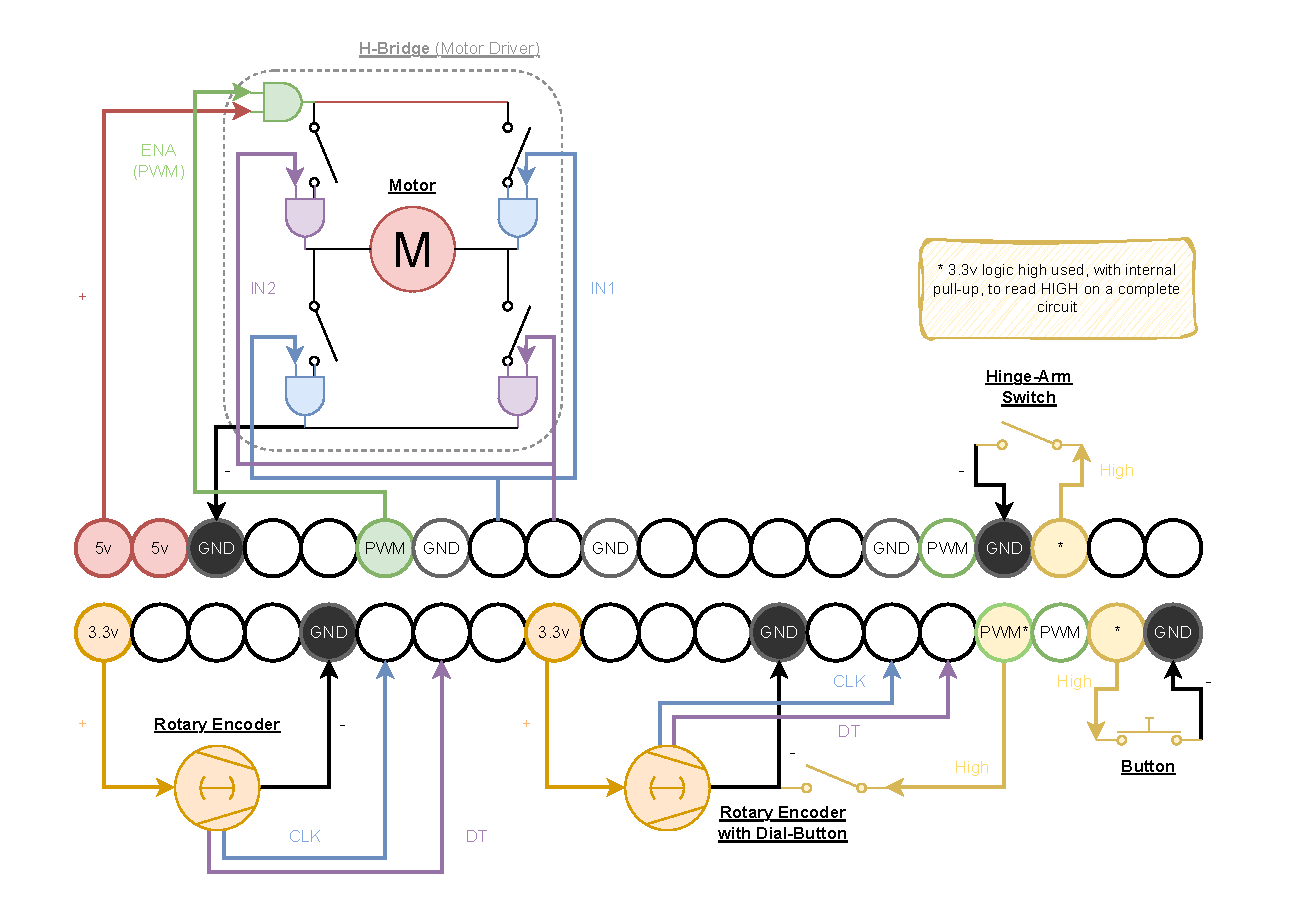
\includegraphics[width=\linewidth]{images/CircuitDiagram.pdf}
                \caption{Circuit diagram of the connected components.}
                \label{fig:circuitDiagram}
                \caption*{Note: The pin layout reflects the actual Raspberry Pi model (cf. Figure~\ref{fig:RPi5Pinout}). Only special (non-standard GPIO) pins needed for this project are coloured (outline), and only used pins are filled. Component positions and details are abstracted for clarity.}
            \end{figure}
        
            \subsubsection{Challenges Encountered}
    
                During the implementation phase of the project, a few problems were encountered when handling the hardware components.
    
                \paragraph{`Measure Twice, Cut Once'}
    
                    Often, when developing software solutions, it is common to use a `trial and error' approach to make a system work. Whilst development is not a mindless task, developers will often just tweak small changes and run the system until it performs correctly, rather than fully designing every single aspect on paper first. For software, in development environments, this is safe to do and even works well as a time-efficient practice. Many technology stacks even accommodate this, with features such as hot-reloading.
    
                    However, when dealing with hardware, this is not the case. During the development of this product there were a few cases where irreparable damage was done to some components due to the use of the above software debugging technique. Whilst configuring the motor to support Pulse-Width Modulation (PWM), the motor driver's jumper connection (which connected the PWM EN input pin to the 5V pin for constant pulse) had to be removed, to allow the PWM GPIO pin to connect. However, after removing the jumper both pins were exposed, and rather than check which one was the correct pin, a rather careless attitude was taken, just guessing which pin it was. This resulted connecting the 3.3V PWM GPIO pin to a live 5V current, which fried the GPIO output.
    
                    Thankfully, the damaged pin was one of four which supports PWM on the RPi 5 model, and so, a backup pin was used.
    
                    This led to greater caution when handling the hardware components afterwards.
    
                \paragraph{Voltage Consumption}
    
                    During early development with the Pi, an unofficial charging cable was used as a power source whilst waiting for the official one to arrive. This cable did not have sufficient wattage for the Pi's specs, and, as a result, it was unable to power the device at high-load without causing the device to turn off.
    
                    To prevent this from being a total blocker, the device was configured to under-clock CPU usage in order to minimise the voltage draw of the device, to minimise how often this would occur.
    
                \paragraph{Overheating}
    
                    Sometimes, during long periods of development, the device would reach very high temperatures. Due to the RPi 5's increased specs over previous models, this is fairly common when running it even for small tasks with only passive cooling. This began to throttle performance during long periods of development and/or testing, however, the solution was simply to setup an active cooling solution. Thankfully, the pins for controlling fan PWM based off of CPU temperatures are separate from the standard GPIO pins, and so did not affect any of the other components.
    
            \subsubsection*{Reflection}
                Hardware prototyping introduced physical risks absent in software -- a fried GPIO pin taught caution the hard way. Pin planning and thermal issues were underestimated early on, but later handled with low-cost fixes and better care.
    
      \subsection{Machine Learning Model} \label{sec:mlImp}
    
            This section outlines the ML models used to classify album artwork, from early CNN prototypes to fine-tuned transfer learning pipelines. The evolution of model architecture, training experiments, and challenges are discussed.
    
            This section covers:
            \begin{itemize}
              \item Initial development using custom CNN models (Baby Ouroboros)
              \item Transition to transfer learning with ResNet18 (Ouroboros)
              \item Experiments with data augmentation and hyperparameter tuning
              \item Two extended architectures: Amphisbaena (multi-head) and Hydra (expandable)
              \item Training constraints and documentation efforts
            \end{itemize}
    
            \paragraph{Tooling and Training Setup}
    
            For implementation of the ML models, PyTorch\footnote{\url{https://pytorch.org/docs/stable/index.html}} was chosen over other libraries (such as TensorFlow,\footnote{\url{https://www.tensorflow.org/api_docs}} Keras,\footnote{\url{https://keras.io/api/}} etc.) due to its superior debugging capabilities and flexibility. Given that this project focused on experimentation rather than production-grade deployment, PyTorch's dynamic computation graph and intuitive design made it a more suitable choice. Experimentation was done through Jupyter notebooks\footnote{\url{https://docs.jupyter.org/en/latest/}}, which aided development due to easily allowing specific code snippets to re-run, and rendering results in-line.
    
            The initial goal was to create a full pipeline that could reasonably run on the Raspberry Pi model. Although it was known that if the dataset grew beyond a toy sample size, training on the Pi would remain technically possible but highly inefficient. With this in mind, all model training and experimentation was instead conducted on a desktop computer utilising an NVIDIA RTX 3060 Ti GPU.\footnote{https://www.nvidia.com/en-gb/geforce/graphics-cards/30-series/rtx-3060-3060ti/\url{https://www.nvidia.com/en-gb/geforce/graphics-cards/30-series/rtx-3060-3060ti/}} Eventually, the idea of training the model on the Pi was dropped entirely, as shown by the prohibitive training times in Table~\ref{tab:trainingTimes}. It remains feasible only for very small models.
    
            \begin{table}[H]
                \centering
                \begin{tabular}{lcc}
                    \toprule
                    \textbf{Scenario} & \textbf{RTX 3060 Ti} & \textbf{Raspberry Pi 5} \\
                    \midrule
                    Single epoch        & $\approx$1.4 seconds     & $\approx$20 minutes \\
                    Full training ($\sim$24 epochs) & $\approx$34 seconds     & $\approx$8 hours \\
                    Hyperparameter search ($\sim$36 runs) & $\approx$21 minutes     & $\approx$216 hours (9 days) \\
                    \bottomrule
                \end{tabular}
                \caption{Average training times for the final \textit{Ouroboros} model on datasets~\ref{data:aug} and~\ref{data:val} ($\sim$1,192 images).}
                \label{tab:trainingTimes}
            \end{table}
    
            \subsubsection{Model Development}
            
            \paragraph{Simple CNN: Baby Ouroboros Model}
    
                In keeping with the experimental learning-through-development approach, the most basic possible CNN model was initially created, as shown in Figure~\ref{fig:BabyOuroboros}. The architecture for this was loosely inspired by early CNN models, particularly LeNet-5 \cite{726791}, and the first implementation was referred to as SimpleCNN.
    
                \begin{figure}[htbp]
                    \centering
                    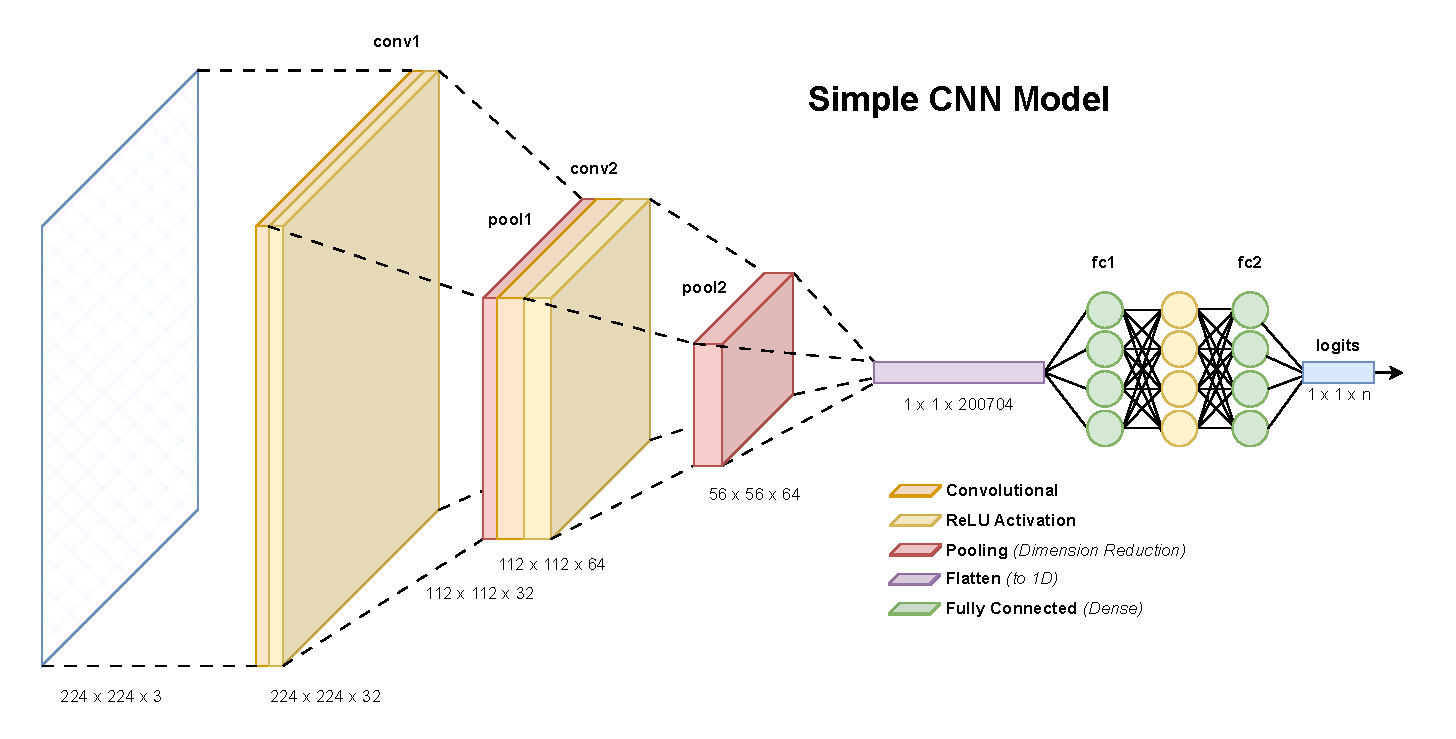
\includegraphics[width=\linewidth]{images/BabyOuroboros.pdf}
                    \caption{Architecture for Baby Ouroboros model (simple CNN protoype).}
                    \caption*{This diagram illustrates the relative sizes and compositions of model blocks, and how they connect across layers. Some details -- such as individual nodes in the fully connected layer -- are abstracted for clarity.}
                    \label{fig:BabyOuroboros}
                \end{figure}
    
                The first iteration of this model (SimpleCNN `Mini') was trained on only the exceptionally small \ref{data:mini} dataset, as a proof of concept. Figure~\ref{fig:SimpleCNN-Mini_Train} shows how the models accuracy increased as training progressed. Whilst the model rather quickly converged and showed good results on the training data (eventually overfitting), the validation dataset's accuracy did climb in slow intervals, but never exceeded 60\%. Whilst this was a good start, it was thought that the problem with this poor generalisation likely came from the sheer small scale of the dataset.
    
                All input data was normalised, per-pixel, according to the same dataset statistic:
                    \[
                    x' = \frac{x - \mu}{\sigma}
                    \]
                where:
                    \begin{itemize}
                        \item \( \mu \) is the mean pixel value \([R,G,B]\) of the dataset.
                        \item \( \sigma \) is the standard deviation of the pixel values.
                    \end{itemize}
    
                Initially, this was calculated as a channel-wide measure of the full combined dataset. However, the standardised ImageNet distribution was also used, with \( \mu = [0.485, 0.456, 0.406] \) and \( \sigma = [0.229, 0.224, 0.225] \), to leverage the greater variation of images it has. Figure~\ref{fig:normalisedArts} shows an example batch of images, normalised to the ImageNet standard.
        
                \begin{figure}[h]
                    \centering
                    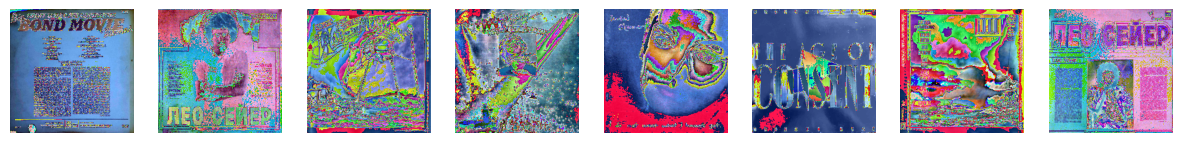
\includegraphics[width=\textwidth]{images/NormalisedArts.png}
                    \caption{Example of normalised dataset batch.}
                    \label{fig:normalisedArts}
                    \caption*{
                        Original artworks are © their respective copyright owners
                        \footnotesize These images have been processed for research/educational purposes and do not intend to infringe upon the original copyrights.
                    }
                \end{figure}
    
                Conforming the data to an external distribution can be a good practice for consistency and compatibility, particularly if there was a chance of later using transfer learning or pre-trained models.
    
                \begin{figure}[h]
                    \centering
                    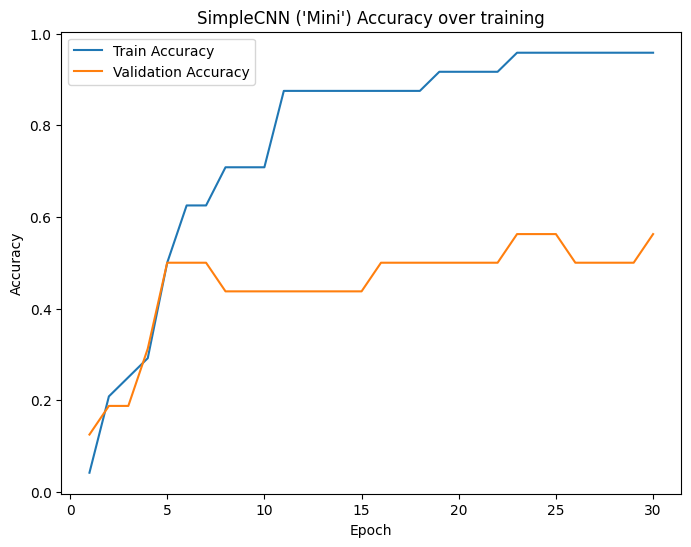
\includegraphics[width=0.75\textwidth]{images/SimpleCNN-Mini_Train.png}
                    \caption{Accuracies of simple CNN architecture on small dataset, per epoch.}
                    \label{fig:SimpleCNN-Mini_Train}
                    \caption*{Higher is better. Training of a SimpleCNN model on \ref{data:mini}; validated against \ref{data:val}.}
                \end{figure}
        
                \begin{figure}[H]
                    \centering
                    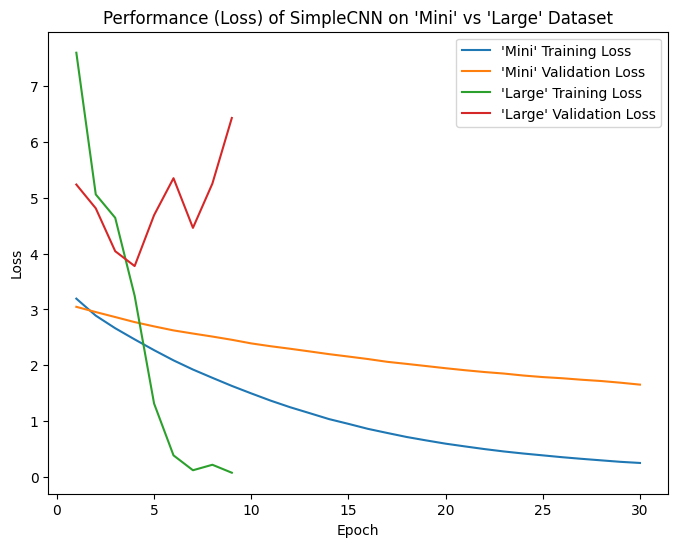
\includegraphics[width=0.75\textwidth]{images/SimpleCNNs_TrainLoss.png}
                    \caption{Comparison of SimpleCNN architecture performance on different sized datasets}
                    \label{fig:SimpleCNNs_TrainLoss-Mini_Train}
                    \caption*{Lower is better. Trained on `Mini' (\ref{data:mini}) and `Large' (\ref{data:large}) datasets; both validated against \ref{data:val}.}
                \end{figure}
    
                The same model architecture was then used to train on a much a larger dataset (\ref{data:large}). However, this model performed very poorly with the sudden increase of data. As shown in Figure~\ref{fig:SimpleCNNs_TrainLoss-Mini_Train}, whilst the loss (`distance' of predictions from the true results) decreases rather smoothly on the smaller dataset, when trying to learn from \ref{data:large}, the model very sharply overfits, and actually worsened in validation performance, never even improving beyond the smaller dataset's initial performance. Figure~\ref{fig:SimpleCNNs_PeakAccuracy-Mini_Train} shows the differences of the best-observed performances of this model architecture across these two training scenarios, showing that performance decreased as the dataset increased.
        
                \begin{figure}[h]
                    \centering
                    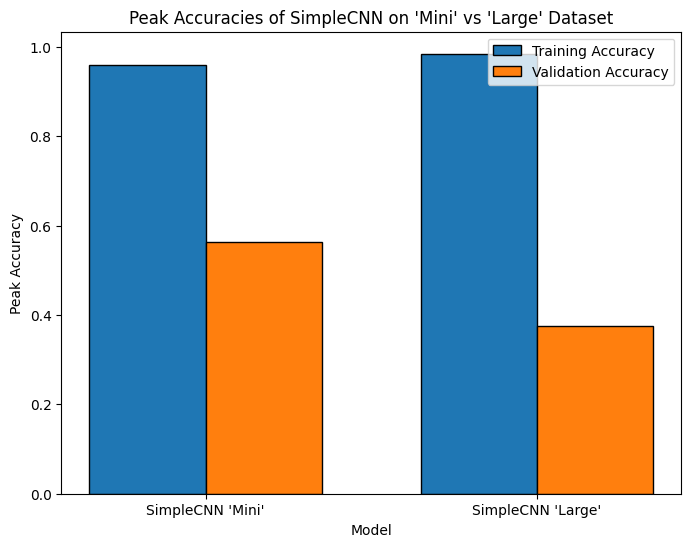
\includegraphics[width=0.75\textwidth]{images/SimpleCNNs_PeakAccuracy.png}
                    \caption{Comparison of best-case SimpleCNN performance on different sized datasets}
                    \label{fig:SimpleCNNs_PeakAccuracy-Mini_Train}
                    \caption*{Trained on `Mini' (\ref{data:mini}) and `Large' (\ref{data:large}) datasets; both validated against \ref{data:val}.}
                \end{figure}
    
                This model performed reasonably on small datasets, but could not scale, and so was labelled as Baby Ouroboros.
    
                In order to improve the results for the large dataset, a deeper model would be required. Various experiments were done with various configurations and depths of model (broadly named DeepCNN), one of which is shown in Figure~\ref{fig:DeepCNN}. However, as the range of albums had increased, even with a greater depth, the feature extraction mechanisms seemed to be lacking. As networks become deeper they require exponentially more data in order to learn sufficiently.
    
                \begin{figure}[h]
                    \centering
                    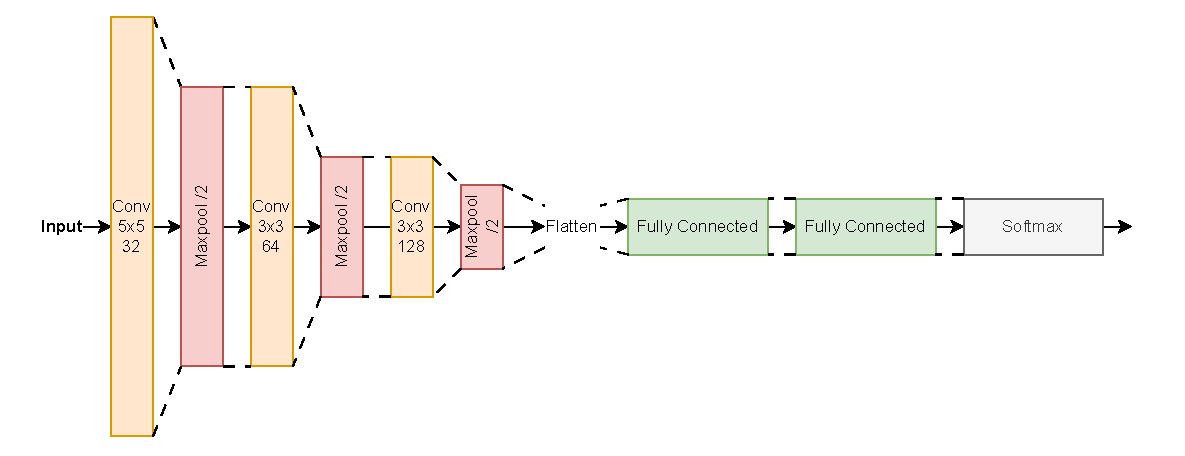
\includegraphics[width=0.95\textwidth]{images/DeepCNN.pdf}
                    \caption{Architecture for an experimental deeper \textit{Baby Ouroboros} model.}
                    \label{fig:DeepCNN}
                    \caption*{
                        The architecture is similar to Figure~\ref{fig:BabyOuroboros}, though some elements have been omitted for simplicity. Earlier figures included certain layers explicitly for educational clarity. All subsequent diagrams adopt this more concise style, consistent with typical publication standards \cite{resnet}.
                    }
                \end{figure}
    
                \paragraph{Transfer Learning: Ouroboros Model}
    
                After the results of the deeper versions of Baby Ouroboros did not prove very fruitful, a new architecture was planned. Rather than trying to train a full model from scratch, it was decided to trial using a feature-extractor from an existing model, which had been trained on a much larger and more generalised dataset. In order to do this, the ResNet18 model was selected, which has been trained on the immense ImageNet library. In theory, a custom solution could have still been trained using this publicly available dataset, with the published parameters and architecture of these models, however, for faster development iterations, it was decided to use the pre-trained feature-extractor, with a custom classifier system built on top of it (see Figure~\ref{fig:OuroborosCNN}).
    
                \begin{figure}[htbp]
                    \centering
                    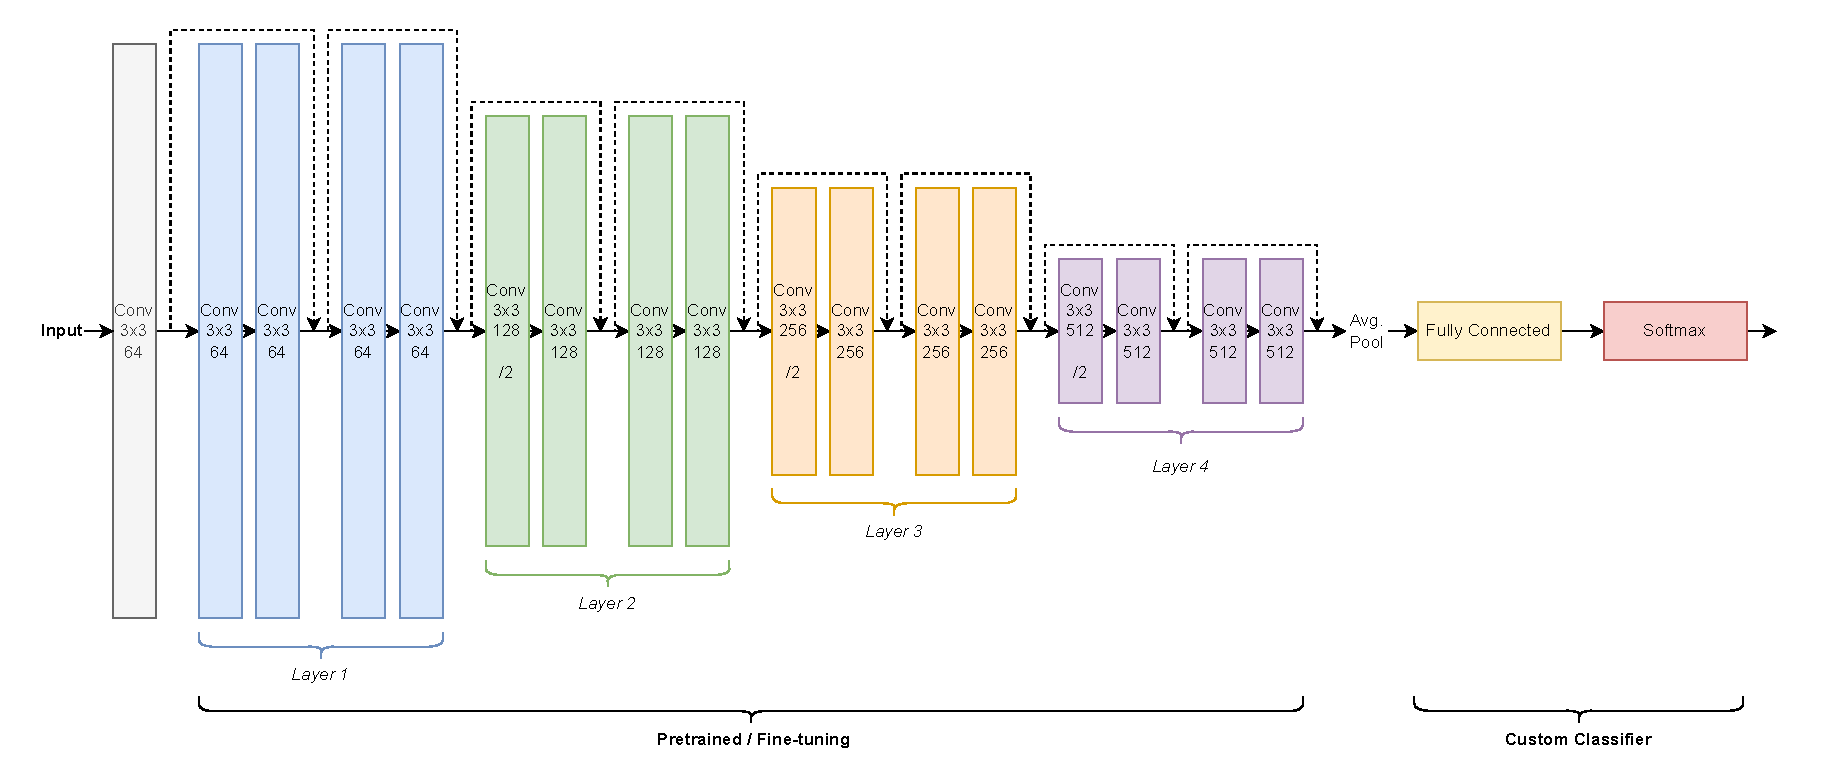
\includegraphics[width=\linewidth]{images/Ouroboros.pdf}
                    \caption{Architecture for Ouroboros model (ResNet18 classifier).}
                    \caption*{Visual style adapted from \cite{resnet}'s ResNet-18 diagram.}
                    \label{fig:OuroborosCNN}
                \end{figure}
    
                \begin{figure}[h]
                    \centering
                    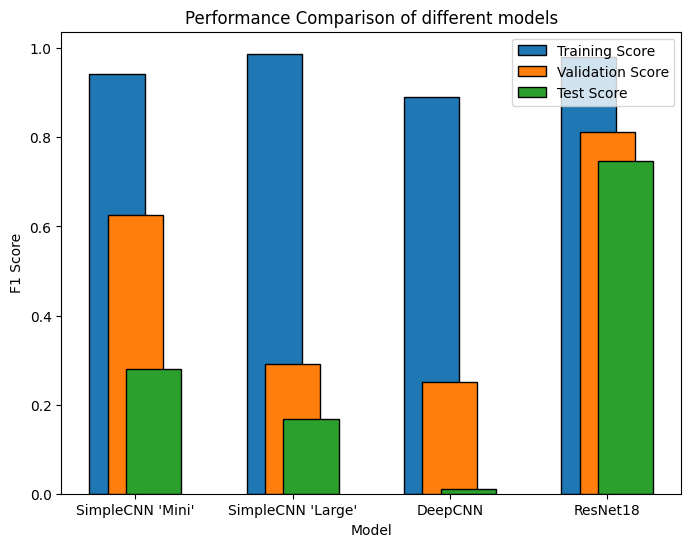
\includegraphics[width=0.75\textwidth]{images/ModelComparison.png}
                    \caption{Average F-Scores for different model architectures and datasets}
                    \label{fig:CNNComp}
                    \caption*{Results are peak observed score, over multiple attempts and datasets. Results shown are of SimpleCNN `Mini' trained on \ref{data:mini}; `Large' on \ref{data:large}; others on \ref{data:aug}. All models validated against \ref{data:val} and tested against \ref{data:test}.}
                \end{figure}
    
                The ResNet18 model, by itself has a powerful feature extractor, however just appending a classifier head on top would yield purely random results, if not further refined through specialised training for the album-recognition task.
    
                \subsubsection{Training Experiments}
    
                    Initially, all ResNet18 weights were frozen, with only the appended classifier head being trained. This approach was intended to avoid heavy biasing and retain pre-trained knowledge, and it already outperformed the in-house DeepCNN model. Further experiments involved selectively unfreezing and fine-tuning varying numbers of layers from the base model to inspect the affect this had on performance.
    
                    \begin{figure}[H]
                        \centering
                        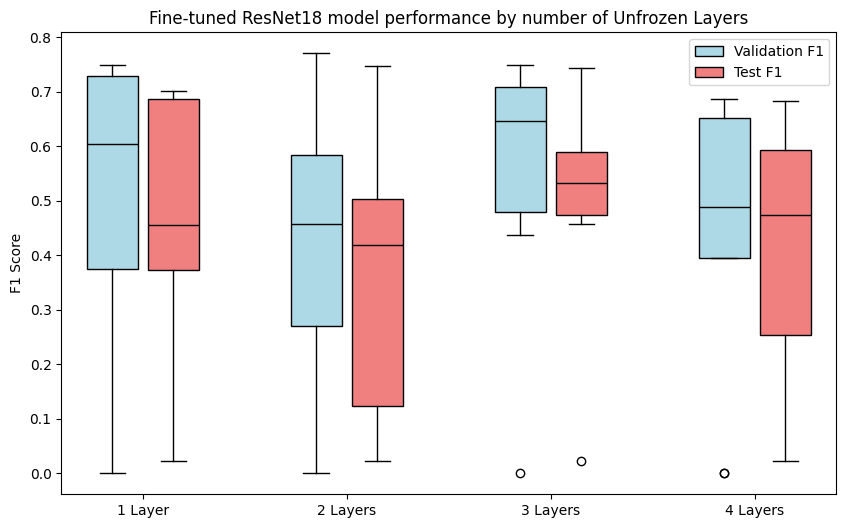
\includegraphics[width=0.8\textwidth]{images/ResNetLayerTests.png}
                        \caption{Boxplot showing the distribution of F1 scores across training epochs for different numbers of unfrozen layers in a fine-tuned ResNet18.} \label{fig:ResNetLayers}
                    \end{figure}
                    
                    As shown in Figure~\ref{fig:ResNetLayers}, the highest validation and test scores were achieved when fine-tuning two layers of the base model. This configuration was therefore preferred in most tests. However, while the 2-layer setup yielded the highest peak results, it also exhibited a broad and low-spread distribution across training epochs. This highlights the importance of choosing the right number of training epochs: stopping too early or training for too long can significantly degrade performance, and so particular care had to be taken in other experimental scenarios using this configuration, to ensure that epoch count was not the deciding factor influencing results.
        
                    \paragraph{Hyperparameter Search}
        
                        A large-scale hyper-parameter grid search was conducted, training the model over various different combinations of value for certain aspects: learning rate, weight decay, number on unfrozen layers, batch size, etc. The results of one test, evaluating different learning rates and weight decays, over each training cycle (epoch), can been seen in Figure~\ref{fig:ResNet_AugGrid}, with the best observed accuracies shown in Figure~\ref{fig:ResNet_AugGridHist}.
                
                        \begin{figure}[h]
                            \centering
                            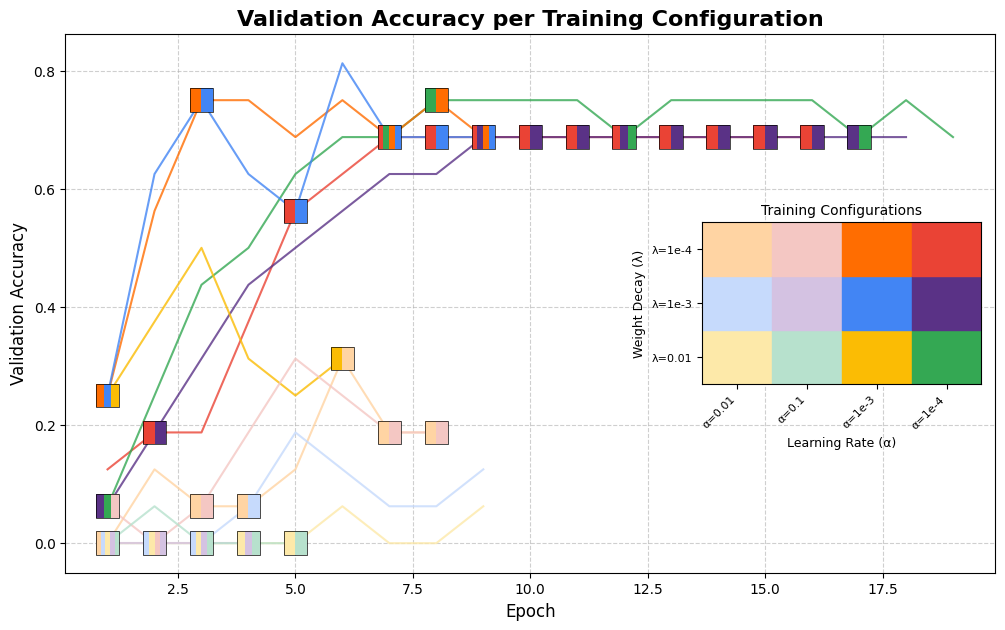
\includegraphics[width=\textwidth]{images/ResNetCNN_AugGrid.png}
                            \caption{Performance results of ResNet18 fine-tuned model hyperparamter grid search}
                            \caption*{Performed on \ref{data:aug} training set (1,176 images) with batch size of 8; validated against \ref{data:val}. Early stopping used when validation loss degraded, so not all configurations ran for equal epochs. Where multiple configurations have the same performance at the same epoch, a square marker indicates which colours are represented.}
                            \label{fig:ResNet_AugGrid}
                        \end{figure}
                
                        \begin{figure}[h]
                            \centering
                            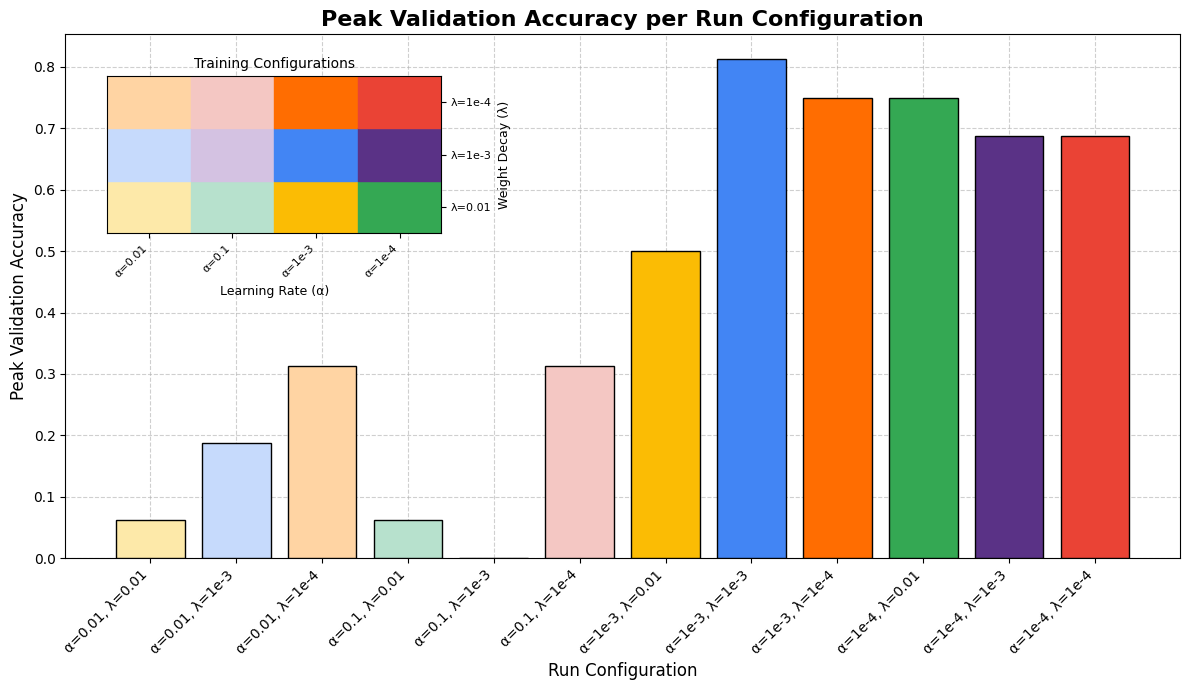
\includegraphics[width=\textwidth]{images/ResNetCNN_AugGridHist.png}
                            \caption{Best-case performance results of ResNet18 fine-tuned model hyperparamter grid search}
                            \caption*{
                                Full set of accuracies during training can be seen in Figure~\ref{fig:ResNet_AugGrid}.
                            }
                            \label{fig:ResNet_AugGridHist}
                        \end{figure}
        
                    \paragraph{Data Augmentation}
        
                        In addition to experimenting with the model's configuration, the data was also investigated. Since the design phase, it was known that this model would likely not need much generalisation techniques, due to being a closed-world task, however, to make the model as robust as possible, data augmentation was still investigated. In a real use case, even though the images will be very similar to their training data, there could be slight fluctuations in rotation, size, and lighting or fading of the artwork. Additionally, some extreme transformations might occur, such as the artwork being fully upside down. In order to make the system handle this, each epoch of training was bolstered with augmented copies with artificial transformations, de-colourings, and cropping taking place (see Figure~\ref{fig:augmentedArts} for an example).
    
                        \begin{figure}[h]
                            \centering
                            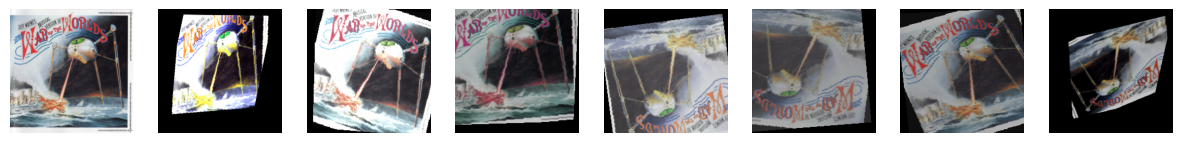
\includegraphics[width=\textwidth]{images/AugmentedArts.png}
                            \caption{Example of augmented dataset batch (without normalisation).}
                            \label{fig:augmentedArts}
                            \caption*{
                                The first image is the unaltered original, whereas the rest of the batch have all be augmented over their rotation, size, cropping, colour, affinity and perspective.
                            }
                            \caption*{
                                Album artwork from \textit{Jeff Wayne's Musical Version of The War of the Worlds} (1978).  
                                \footnotesize Used for research/educational purposes. All rights remain with the original copyright holders.
                            }
                        \end{figure}
    
                        This augmentation was generated `on-the-fly' during training, meaning no modified image was saved or stored beyond the training epoch. Additionally, this meant that each epoch had slightly different variations it was learning on. This made the training process better for generalisation, serving as a forced dropout of seen images; however, the training process became slower, requiring more training epochs to accurately learn from the data, as well as the dataset now being scaled to be larger, increasing the time taken to train.
    
                        Even with GPU optimisation, as the dataset multiplied in size, it became infeasible to store the data within the available VRAM at once, and so batch sizes had to be decreased from ~32 to ~8, in most cases, further slowing the training process.
    
                        This `on-the-fly' approach also had drawbacks, as it required additional rendering computations in every epoch cycle, but the performance gains made the extra time taken a worthwhile trade-off.
        
                    \paragraph{Data Hyperparamaters}
    
                        Not only was the model configuration rigorously tested under various alterations, but also the training dataset.
    
                        One notable requirement of a CNN model, is that all input data must be the same size, that is, the images must all be of uniform dimensions. The initial baseline used was \(244×244\) pixels (noted as \(244^2\)px throughout), though it was theorised that greater fidelity versions of images could improve quality.
    
                        As per Figure~\ref{fig:CNNSize_Perf}, various image sizes were tested on the ResNet18-based model, to varying degrees of observed success. Whilst the \(124^2\)px size did have the highest peak in performance, the \(244^2\)px was most consisent in its performance. The more extreme sizes seemed to perform most poorly, likely due to the smallest images having too great of a loss in details to be learnable, whereas the larger images were likely subject to too much noise and variation, as well as potentially requiring more epochs or a deeper network with larger convolution kernels to adequately learn details.
            
                        \begin{figure}[h]
                            \centering
                            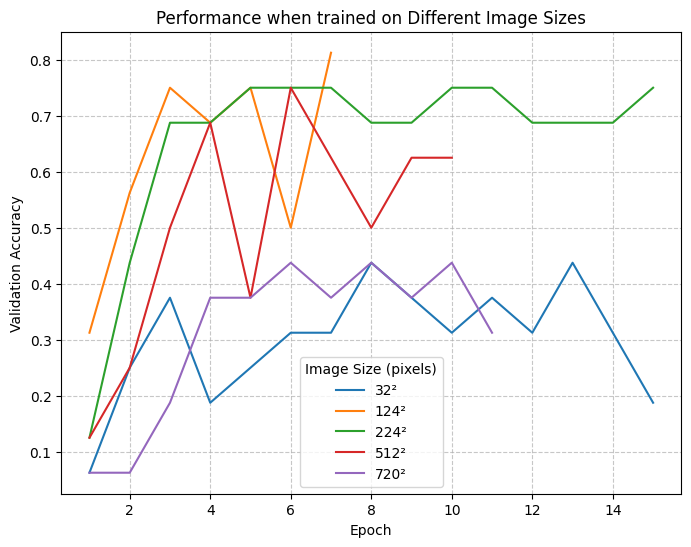
\includegraphics[width=0.85\textwidth]{images/CNNSize_Perf.png}
                            \caption{Model accuracy per training epoch, using different image sizes}
                            \label{fig:CNNSize_Perf}
                            \caption*{Results are averaged over multiple attempts.}
                        \end{figure}
    
                        The \(124^2\)px, \(244^2\)px, and \(512^2\)px input sizes were also tested. As shown in Figure~\ref{fig:CNNSize_Time}, training time scaled roughly with image area (\(x^2\)), which is expected given that convolution operations are inherently per-pixel, even when batched. The \(244^2\)px resolution was chosen as the primary input size, offering consistent performance with lower training times than \(512^2\)px, while outperforming \(124^2\)px.
    
                        Additionally, when switching to utilise the ResNet feature extractor, the \(244^2\)px was especially the best-performing, as this was the input size used for the model's initial training.
                
                        \begin{figure}[h]
                            \centering
                            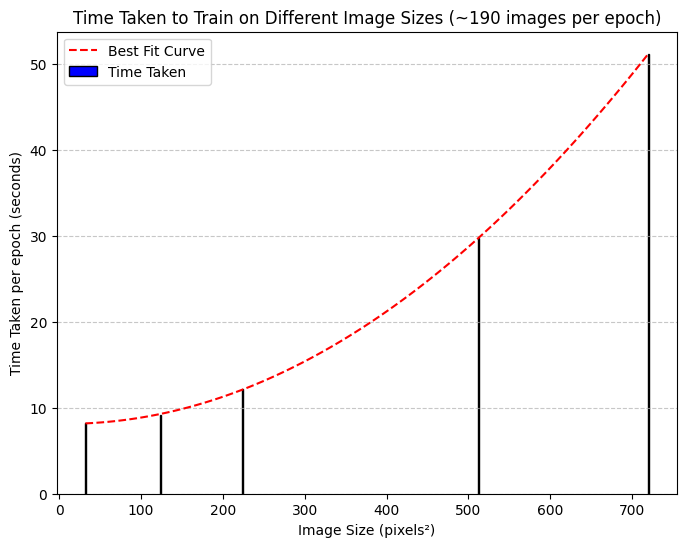
\includegraphics[width=0.85\textwidth]{images/CNNSize_Time.png}
                            \caption{Average training time for different image sizes}
                            \label{fig:CNNSize_Time}
                            \caption*{Results are averaged over multiple attempts.}
                        \end{figure}
    
            \subsubsection{Extended Architectures}
    
                \paragraph{Amphisbaena (Multi-Headed)}
    
                The Ouroboros model, using the ResNet18 architecture, was additionally built upon to have two classification heads, allowing the model to learn different categories for the same items. The architecture was mostly the same as Ouroboros, except for an additional classifier head (see Appendix~\ref{app:img}, Figure~\ref{fig:AmphisbanaeCNN}), which allowed the model to, in addition to learning the album, learn a de-coupled artist value. Using a single network, diverging into two output heads at the end allowed for shared learning from feature extraction, and reduced redundant duplication of resource-heavy processes (for example, this task could be done with two fully separate models, but would double the training time).
    
                This was largely done as an experimental feature, as it was unknown how well an artist can be detected, on unseen data, from other albums of the same artist. Whilst author classification is an area being explored for visual artists, this is a much more generalised task for album covers, as two albums by the same musician may feature two drastically different artworks produced by different artists, with little-to-no overlap. However, some musicians do have stylistic consistency in their albums covers. A notable example in pop culture is Ed Sheeran, whose albums often feature mathematical symbols and paint effects (see Appendix~\ref{app:Cult}, Figure~\ref{fig:EdMeme} for a comedic example). Additionally, albums by the same musician may consistently feature a logo, brand, or even the their likeness, which could be enough information for a deep model to learn from. And, finally, many album arts are done by the same artist for a single performer or band, and so even stylistic aspects could still be beneficial.
    
                \begin{figure}[h]
                    \centering
                    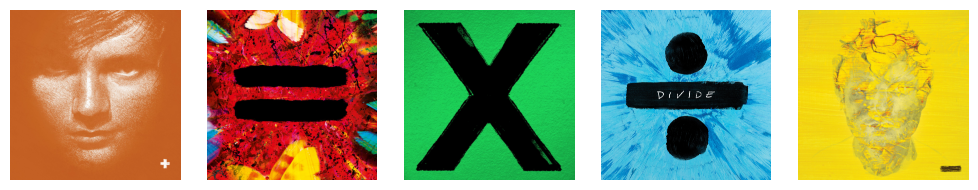
\includegraphics[width=0.6\textwidth]{images/EdAlbums.png}
                    \caption{Album covers of Ed Sheeran's studio albums}
                    \label{fig:EdAlbums}
                    \caption*{+ (2011), = (2021), × (2014), ÷ (2017), and − (2023). \\ Images © Asylum Records / Atlantic Records. Retrieved from Cover Art Archive. Used for research/educational purposes. All rights remain with the original copyright holders}
                \end{figure}
    
                After some experimentation, it was found that the model was able to achieve some level of success. As a proof of concept, as part of the \ref{data:large} dataset, four of Ed Sheeran's albums were included. These images (the first four, from the left, in Figure~\ref{fig:EdAlbums}) were able to learn enough information such that the − (2023) album (right-most image) included in \ref{data:test2} was able to be correctly identified as an Ed Sheeran album (64\% confidence).
    
                It is worth noting that this use case is a particularly ideal one, however, with Ed Sheeran's albums all being very uniformly consistent.
    
                The aim to experiment with additional classification channels, such as genre or decade, proved unviable within the available time and was therefore omitted, along with further testing with different artists.
    
                \paragraph{Hydra (Expandable)}
    
                The creation of the dynamically-expandable classification system was conducted, though, due to time constraints, only minimal experimentation was conducted. The use-case for this model was that, if a user had a large collection and had set up this system to classify them, but then bought a new record, they would have to fully re-train a new model from scratch, to accommodate the new addition. Furthermore, if the model was performing poorly on some albums, the user would, theoretically, be able to inform the system of this, essentially acting as a manual annotator, which could be used to give higher weightings to these albums, to tune the model to match user expectations. This goal of high-level model customisation was challenging, however.
    
                At first, the idea was to simply fine-tune the previously trained models, using a new collection of data. But, it was quickly found that catastrophic data loss occurred when altering weights without the original training images to validate them.
    
                In order to avoid the retention or re-downloading of copyrighted images to be required for this system to work, instead a matrix database was created. The classification model essentially has two components: a feature extractor and a classifier. The idea was to, once initial training was complete, run each training image through the feature-extractor only, and to store the numerical tensor (the embedding) in this database. Then, if a future revision of the model was desired, the feature extractor could be frozen, then classifier could be re-initialised to allow an additional album, and the already-extracted features could be fed directly into the classifier, alongside the new data going through the full model, to ensure training saw both sets of data (illustrated in Figure~\ref{fig:HydraCNN}).
    
                Whilst this technique showed better results, it was still prone to catastrophic data loss, either biasing towards the new data, or the original data. Freezing the feature extractor, whilst allowing to remember old features better, prevented the model from being able to correctly learn new albums; on the other hand, removing this constraint resulted in the previously extracted data sometimes being almost-random in accuracy -- sometimes performing okay, but other times not; with no consistent way of ensuring ideal performance.
    
                \begin{figure}[h]
                    \centering
                    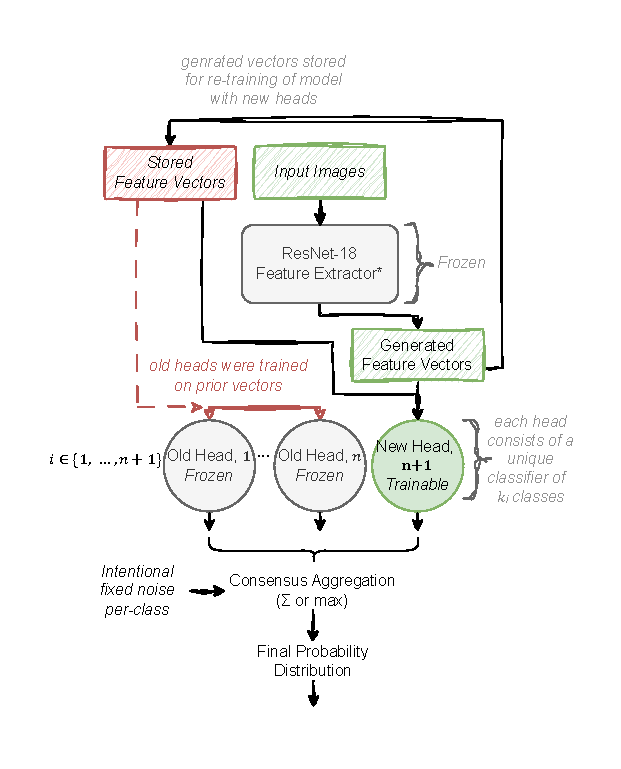
\includegraphics[width=0.75\linewidth]{images/Hydra.pdf}
                    \caption{Architecture for \textit{Hydra} model (expandable classifiers).}
                    \label{fig:HydraCNN}
                    \caption*{
                        A PNN enabling dynamic class extension; a frozen ResNet-18 extracts features for multiple heads (\(i \in \{1, \dots, n+1\}\)), each trained on distinct class subsets. Outputs are aggregated (sum or max) into a final probability distribution. Stored vectors allow future head training without original inputs.
                    }
                    \caption*{* For a detailed breakdown of the feature extractor, refer to Figure~\ref{fig:OuroborosCNN}.}
                \end{figure}
    
                For this, a PNN architecture was created, allowing a dynamic number of heads to operate in parallel, using a weighted consensus approach to generate a single classification, as shown in Figure~\ref{fig:HydraCNN}. This idea still utilised a single, frozen feature extractor, utilising the retained embeddings, however, rather than replacing the classifier, a new classifier was added in tandem to the original one. Then, during training, the two heads were weighted, through cross-entropy loss, so that the final result was the `consensus' of the two. Essentially, the original model was preferred, unless the second model had a high degree of confidence that it was a new class, in which case, the system delegated to the newer head if, and only if, the original head was not also highly confident.
    
                This system showed promising improvement over the early attempts, yet performance degradation was still significant, with the model dropping from $\approx$80\% confidence on the initial images to $\approx$30\% (though, accuracy was maintained in the very small testing sample set used). This showed that the dynamic approach was at least, potentially,  viable for a full-scale solution. Though, due to time constraints, no further experimentation was done on this concept.
    
                A major issue with the initial vision was that, if users were to update their model, the training would ideally run on-demand on the Pi. However, given the reliance on a vector database and a deep model, this would likely be too slow on the SBC. As such, a scheduled, once-per-day cycle could be considered -- echoing existing strategies used reduce load under constrained resources~\cite{gonzalez2019cernbox}.
    
            \subsubsection{Documentation}
    
                Additionally, in order to make the models clear and distinct from one another, as well as being potentially useful to other developers, a model card \cite{Mitchell_2019} was created\footnote{The model card for the Ouroborus model is provided in Appenidx~\ref{sec:mcard}, alongside links to the others.}, for each.
            
            \subsubsection{Challenges Encountered}
    
                On the 8th of October 2024, the Internet Archive suffered a significant cyberattack causing widespread outages, including the Cover Art Archive \cite{forbes2024}. As this archive, run jointly with MusicBrainz, was the primary source for the model training data, this prevented downloading any data to expand the dataset.
    
                The outage lasted weeks, with services gradually restored; the Cover Art Archive returned after the 21st of October \cite{archiveBlog2024}. Fortunately, a small dataset had already been gathered, along with physical media, allowing limited model training while development continued.
    
                Had the outage persisted, switching sources would have been necessary. Last.fm was shortlisted as a backup. Although services stabilised, further outages were reported post-development \cite{hackread2024}.
    
            \subsubsection*{Reflection}
                The early CNNs underperformed at scale, but transfer learning delivered strong results with less training overhead. Attempts at less redundant systems (Amphisbaena) and dynamic expansion (Hydra) were promising, though not production-ready -- future work could refine this into a user-adaptive system fit for deployment.
    
    %%%%%%%%%%%%%%%%%% SECTION 5 %%%%%%%%%%%%%%%%%%
    \section{Results} % edit section heading as appropriate
        % results of soft/hardware testing
        % screenshots of UI / program output
    
        This section presents the completed outputs of the system: a functional full-stack application, an interactive hardware artefact, and their seamless integration into a hybrid user experience. It provides a visual and descriptive overview of each element, highlighting what was achieved and what functionality is offered to the end user.
        
        Detailed evaluation of their effectiveness, usability, and alignment with the project aims is presented in Section~\ref{sec:evaluation}.
        
        \subsection{Software Artefact}
    
            The system includes a complete browser-based application designed for playback control, visual feedback, and media interaction. It supports both a local host interface (projected onto the device) and external client interfaces (via mobile or desktop browsers), all communicating with a central backend.
    
            \paragraph{Host Interface}
    
            The host interface runs on the local device and is the main control centre of the system. It provides visual feedback during playback. The UI is minimal by default, giving only the same information a physical vinyl on a player would: its centre label artwork; maintaining an unobtrusive appearance. Additional UI elements and controls remain hidden by default and only appear with active input (e.g., mouse movement), showing greater details (album art, album name, track name, etc.) and providing a digital method to achieve each use case (as per Figure~\ref{fig:umlusecase}).
    
            Figures~\ref{fig:hostQuiet}–\ref{fig:hostGui} show the host view with and without active UI overlays.
    
            \begin{figure}[h]
                \centering
                \begin{minipage}[b]{0.45\textwidth}
                    \centering
                    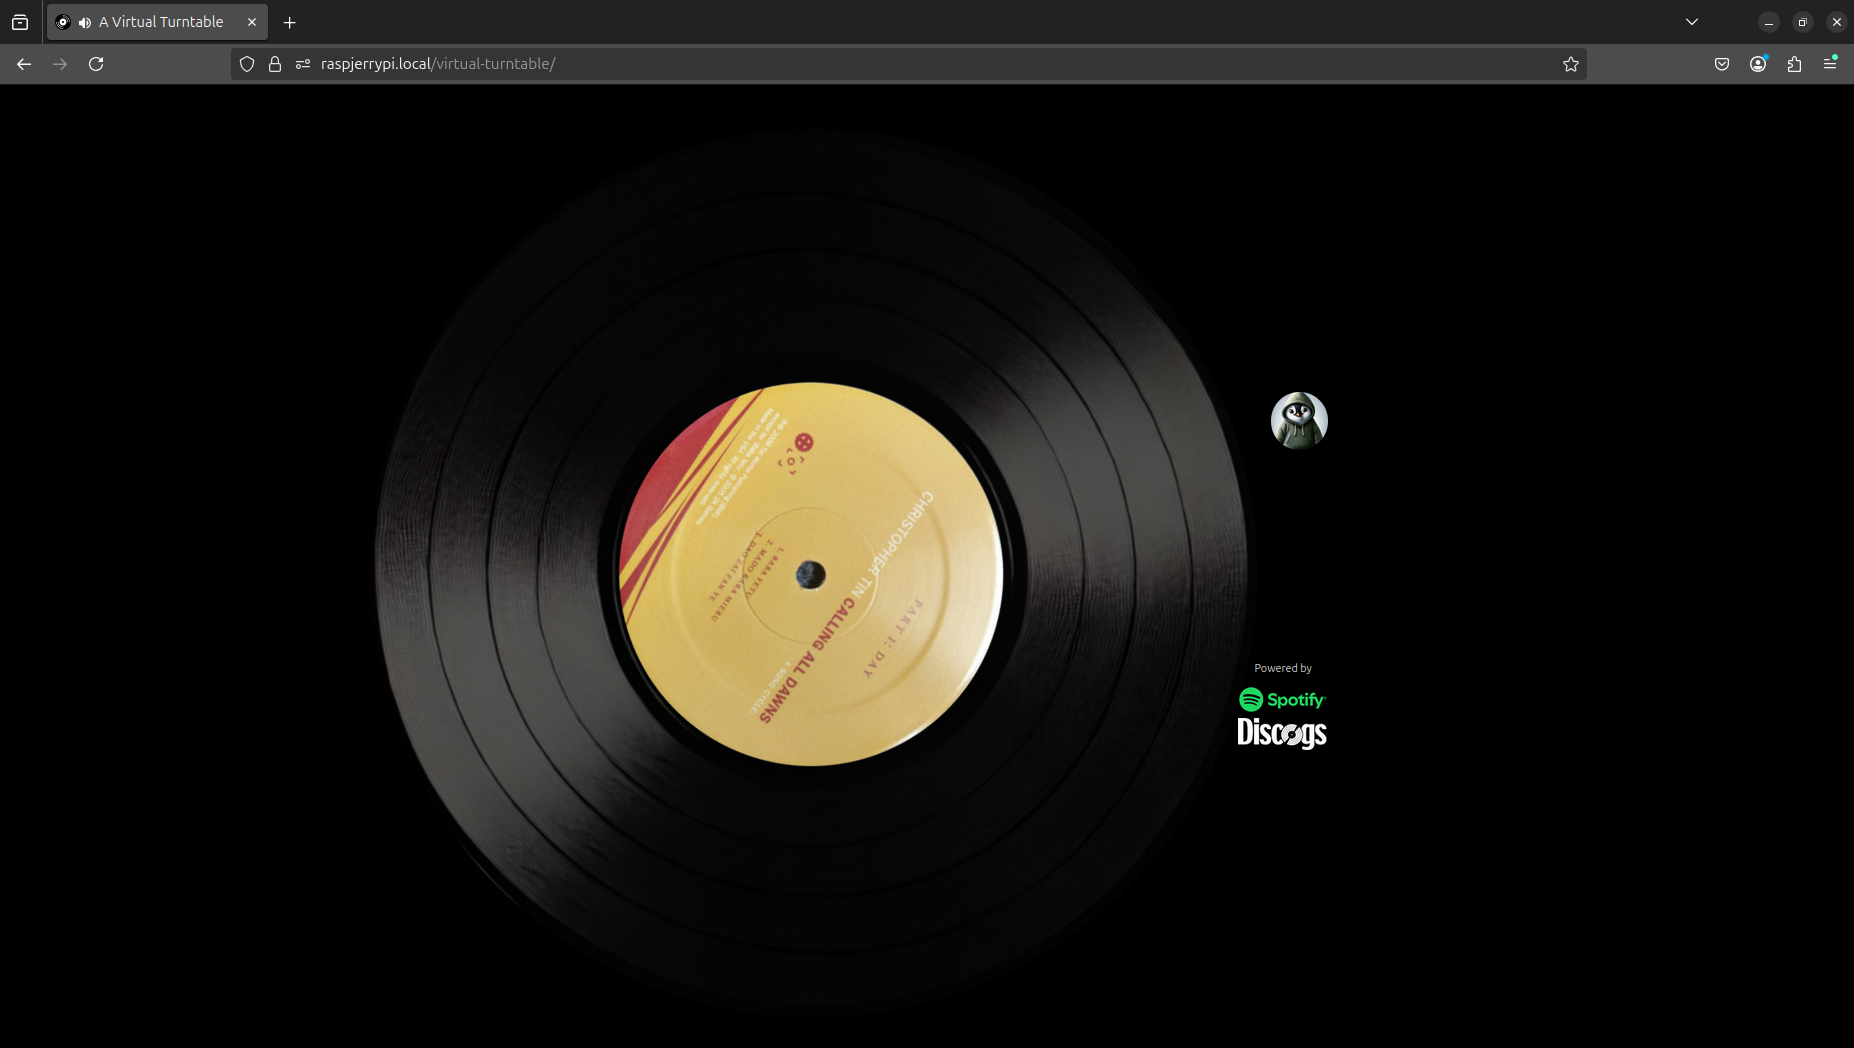
\includegraphics[width=\textwidth]{images/screenshots/HOST_Quiet.png}
                    \caption{Host client playing a track}
                    \label{fig:hostQuiet}
                \end{minipage}
                \hfill
                \begin{minipage}[b]{0.45\textwidth}
                    \centering
                    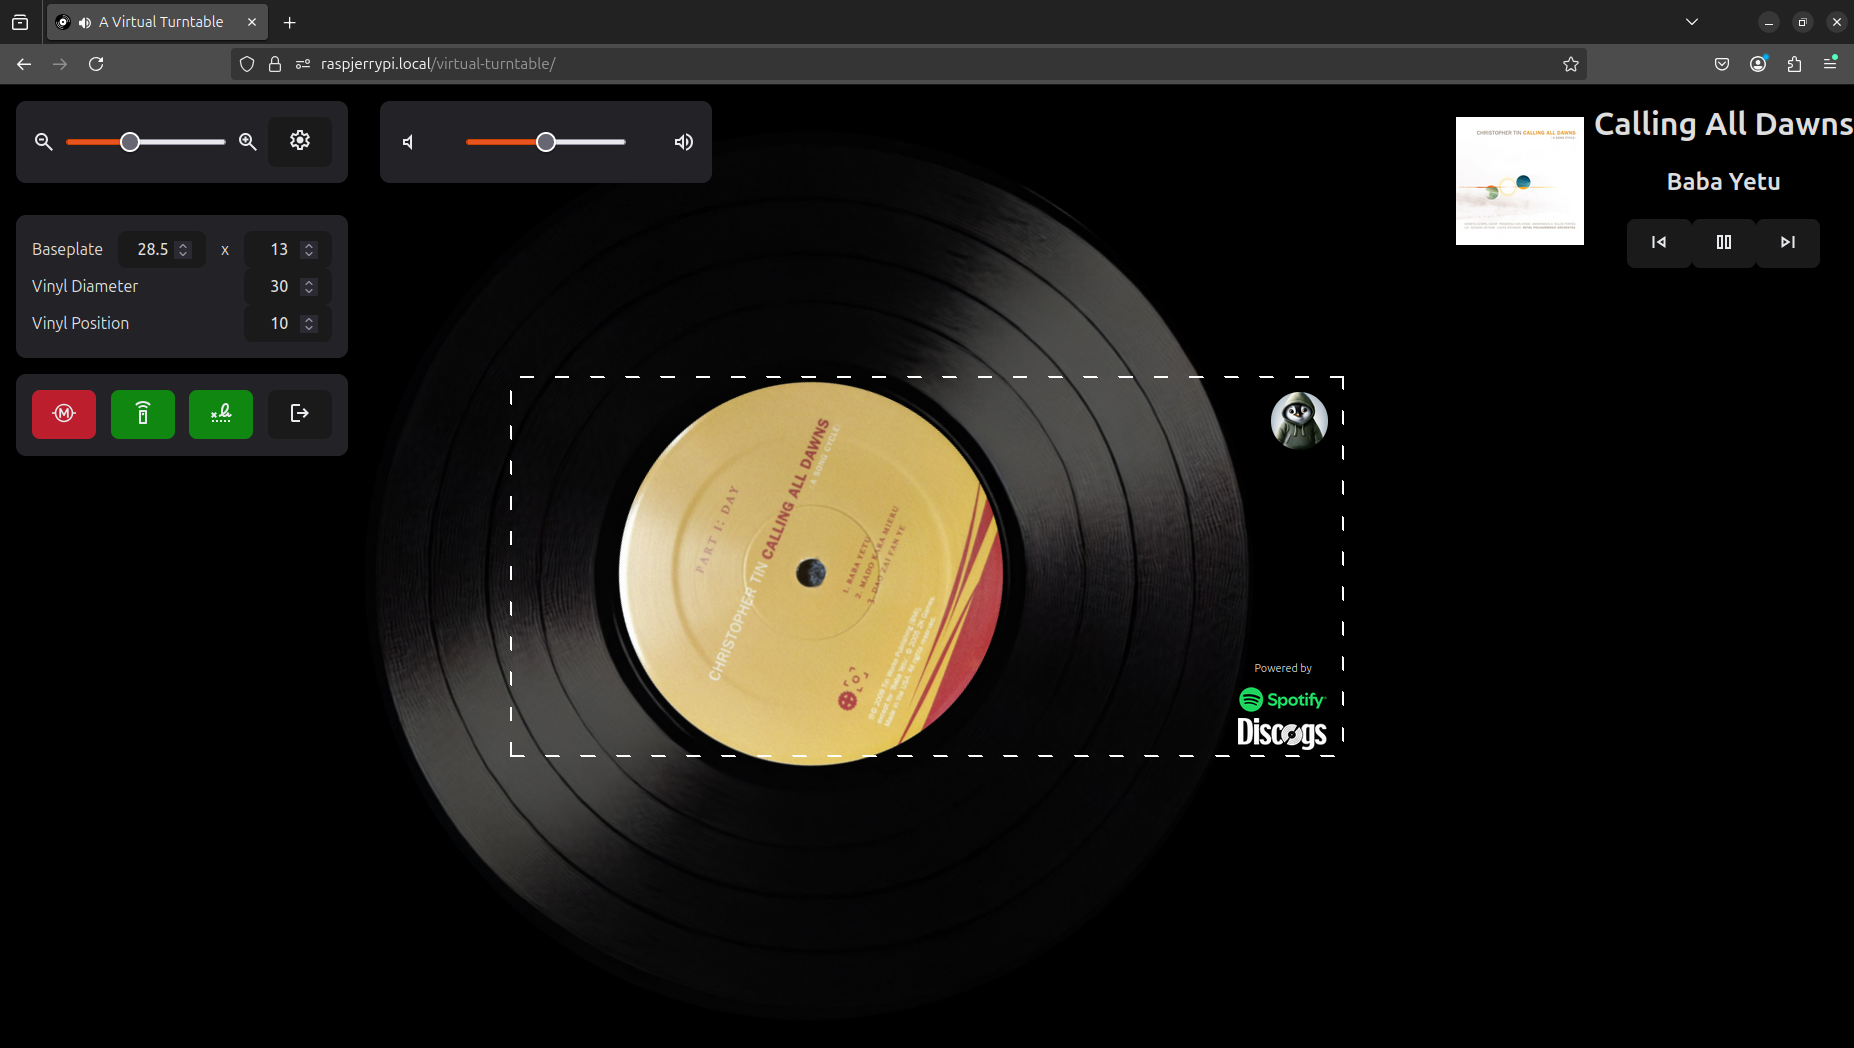
\includegraphics[width=\textwidth]{images/screenshots/HOST_GUI.png}
                    \caption{Host client playing a track, with UI overlays}
                    \label{fig:hostGui}
                \end{minipage}
            \end{figure}
    
            \paragraph{Remote Client Interface}
    
            The system also provides a web-based remote interface, enabling mobile phones or desktop browsers to connect over the local network. These clients replicate the core controls of the host -- such as play/pause, volume, track skip, and album scanning -- allowing accessible, shared interaction. Figures~\ref{fig:laptop}–\ref{fig:phone} show examples of remote clients in use on different devices.
    
            \begin{figure}[h]
                \centering
                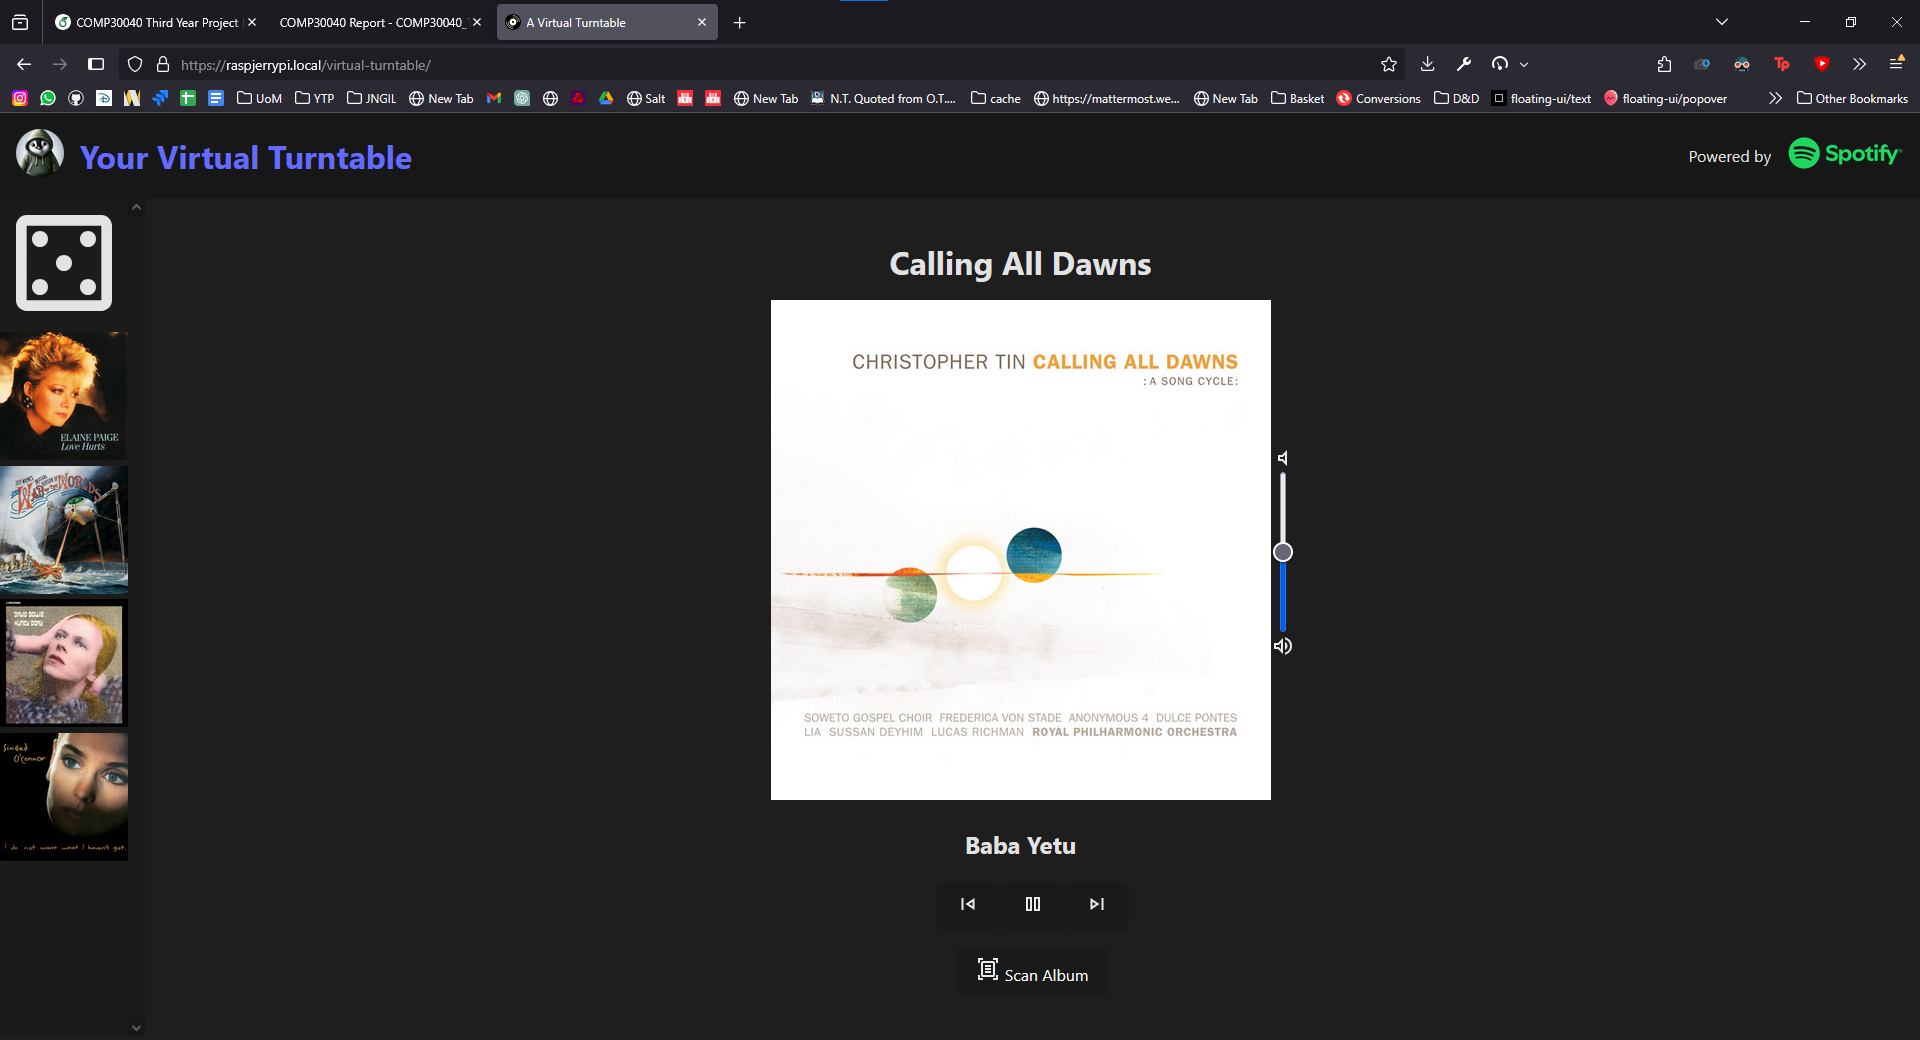
\includegraphics[width=0.45\textwidth]{images/screenshots/LAPTOP.png}
                \caption{Screenshot of a remote client (PC) connected to the host}
                \label{fig:laptop}
            \end{figure}
            
            \begin{figure}[h]
                \centering
                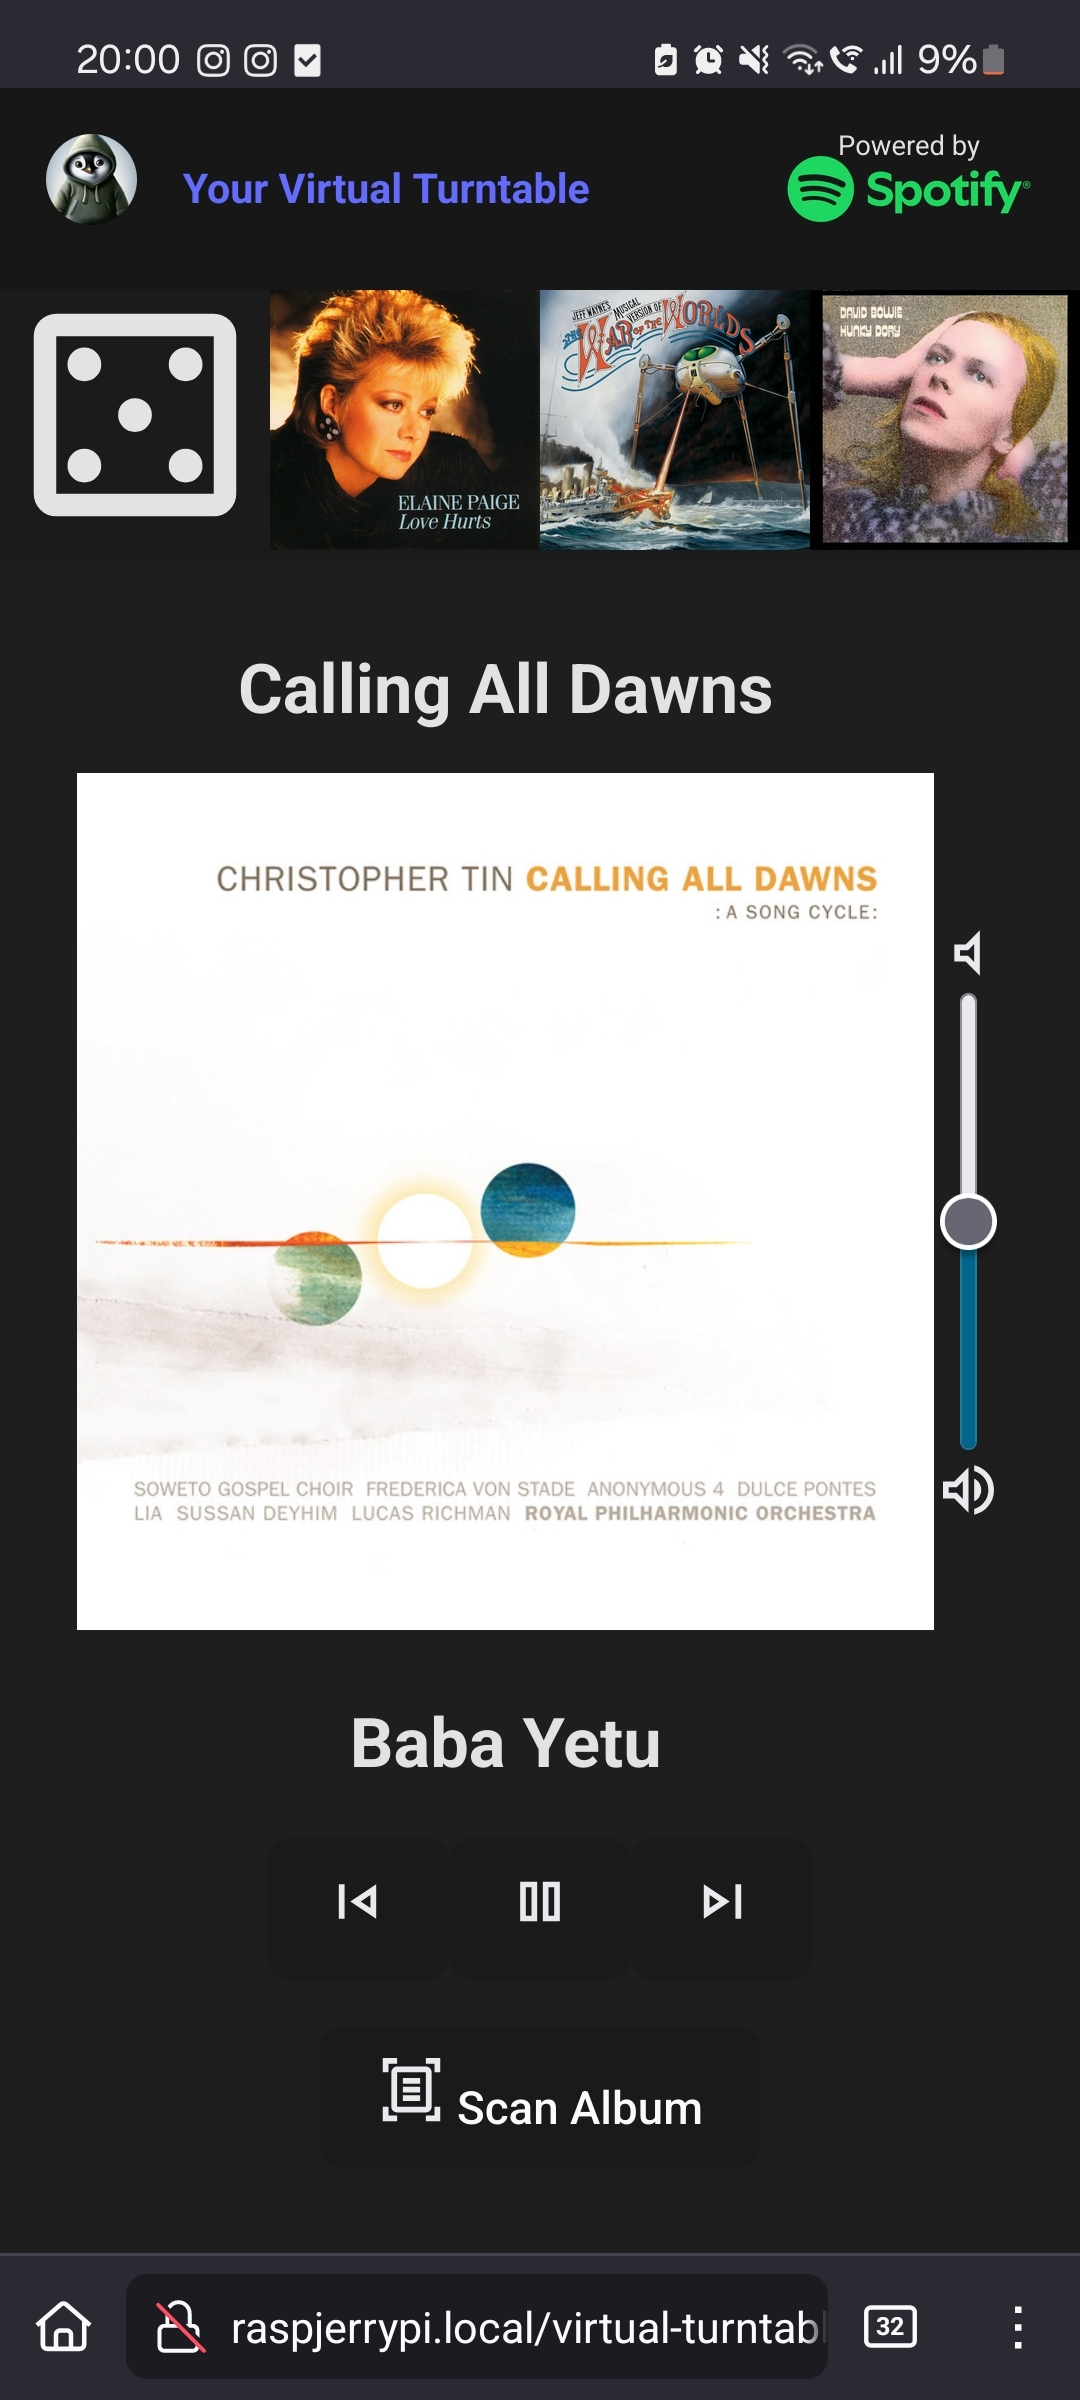
\includegraphics[width=0.35\textwidth]{images/screenshots/PHONE.jpg}
                \caption{Screenshot of a remote client (mobile) connected to the host}
                \label{fig:phone}
            \end{figure}
    
            \paragraph{Classification Model}
    
            The delivered model was a fine-tuned ResNet18 CNN, referred to as Ouroboros, trained on a curated dataset of album covers. It used a partially-frozen feature extractor from ImageNet pretraining, with a custom classifier head trained for album identification. Data augmentation, hyperparameter tuning, and image normalisation were used to optimise performance. The model was integrated into the backend and served via an API for live classification.
        
        \subsection{Hardware Artefact}
    
            The system is built into a physical Raspberry Pi-powered device. The unit includes tactile controls such as a rotary dial, physical button, and hinged `playback arm' -- each mapped to corresponding actions (e.g., play/pause, track skip, scan).
    
            A webcam is mounted to capture album cover images for recognition, and a motor spins a disc during playback, creating a dynamic and nostalgic effect. Figures~\ref{fig:product}–\ref{fig:bottom} show the unit from various perspectives, demonstrating form factor and component layout.
    
            \begin{figure}[H]
                \centering
                \begin{minipage}[b]{0.45\textwidth}
                    \centering
                    \includegraphics[width=\textwidth]{images/photos/product_1.jpg}
                \end{minipage}
                \hfill
                \begin{minipage}[b]{0.45\textwidth}
                    \centering
                    \includegraphics[width=\textwidth]{images/photos/product_2.jpg}
                \end{minipage}
                \caption{The finished build, with playback arm raised (left) and lowered (right).}
                \label{fig:product}
            \end{figure}
    
            \begin{figure}[H]
                \centering
                \begin{minipage}[b]{0.45\textwidth}
                    \centering
                    \includegraphics[width=\textwidth]{images/photos/profile_TOP.jpg}
                    \caption{Top-down profile of the device (circuitry exposed)}
                    \label{fig:top1}
                \end{minipage}
                \hfill
                \begin{minipage}[b]{0.45\textwidth}
                    \centering
                    \includegraphics[width=\textwidth]{images/photos/profile_TOP3.jpg}
                    \caption{Top-down profile of the device (with vinyl attached and  playback arm lowered)}
                    \label{fig:top2}
                \end{minipage}
            \end{figure}
    
            \begin{figure}[H]
                \centering
                \begin{minipage}[b]{0.45\textwidth}
                    \centering
                    \includegraphics[width=\textwidth]{images/photos/profile_FRONT.jpg}
                    \caption{Front profile of the device}
                    \label{fig:front}
                \end{minipage}
                \hfill
                \begin{minipage}[b]{0.45\textwidth}
                    \centering
                    \includegraphics[width=\textwidth]{images/photos/profile_BACK.jpg}
                    \caption{Back profile of the device}
                    \label{fig:back}
                \end{minipage}
            \end{figure}
    
            \begin{figure}[H]
                \centering
                \begin{minipage}[b]{0.225\textwidth}
                    \centering
                    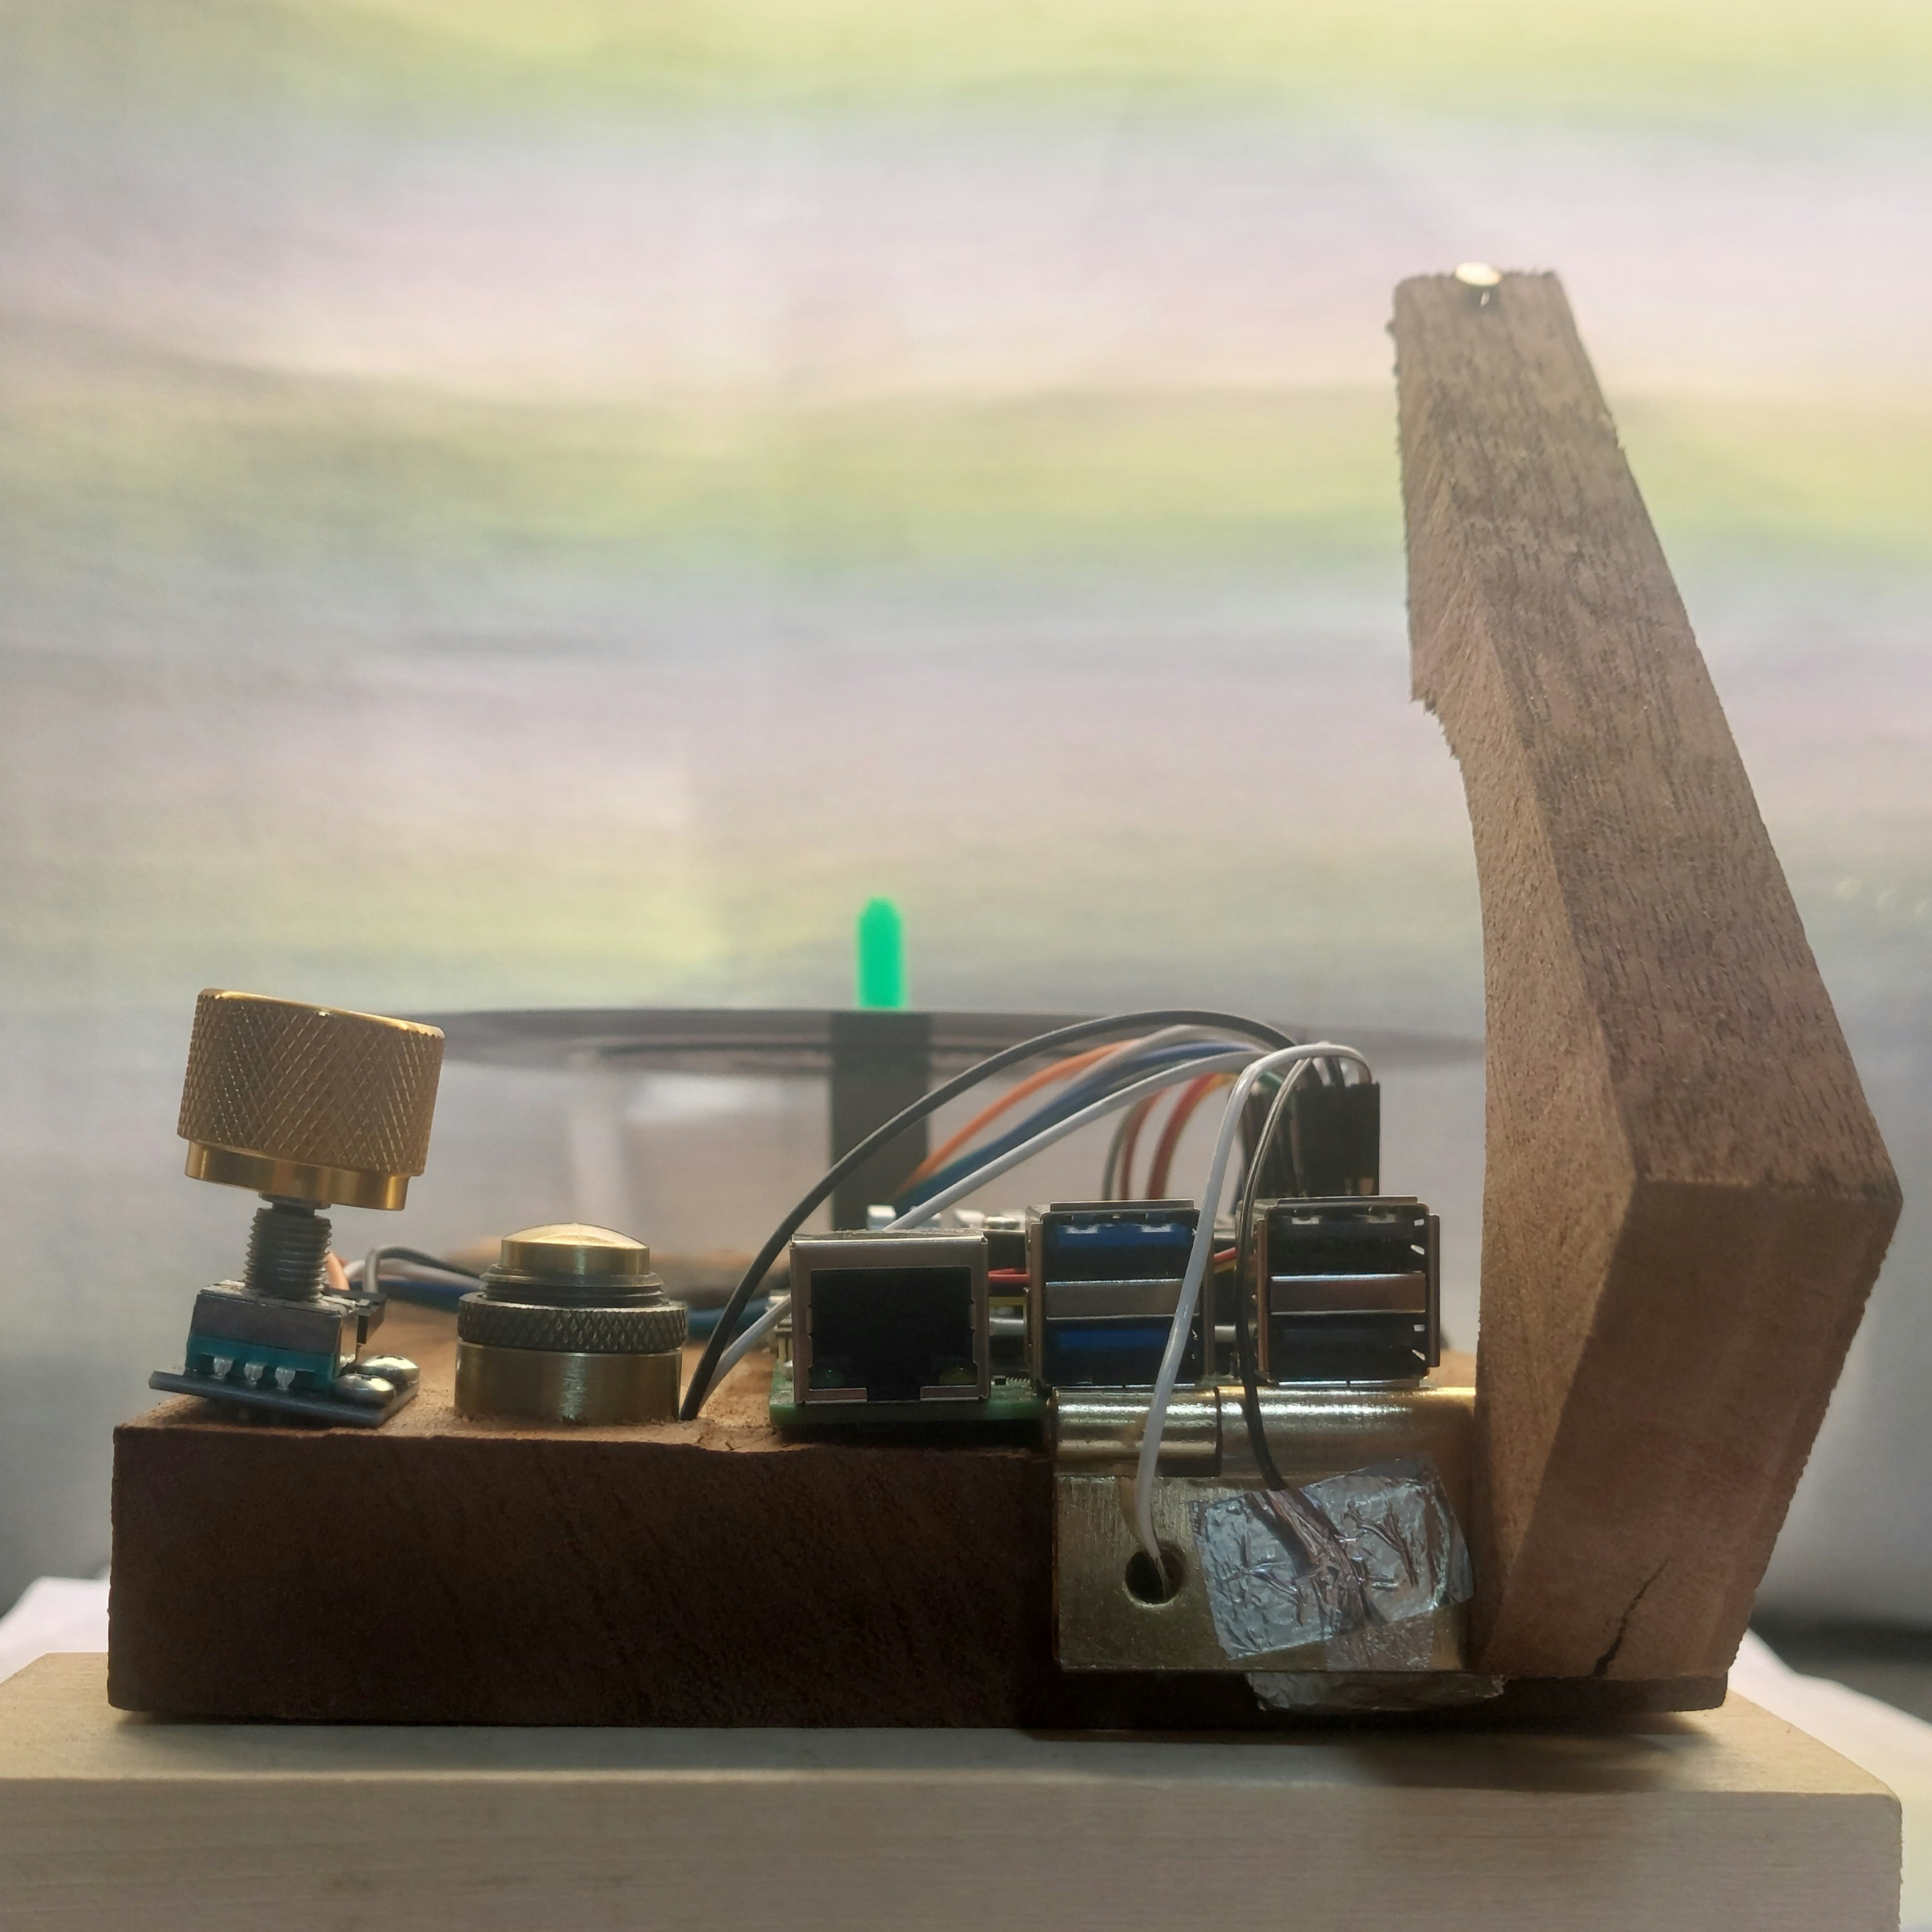
\includegraphics[width=\textwidth]{images/photos/profile_SIDE.jpg}
                    \caption{`Near' side profile of the device}
                    \label{fig:side1}
                \end{minipage}
                \hfill
                \begin{minipage}[b]{0.225\textwidth}
                    \centering
                    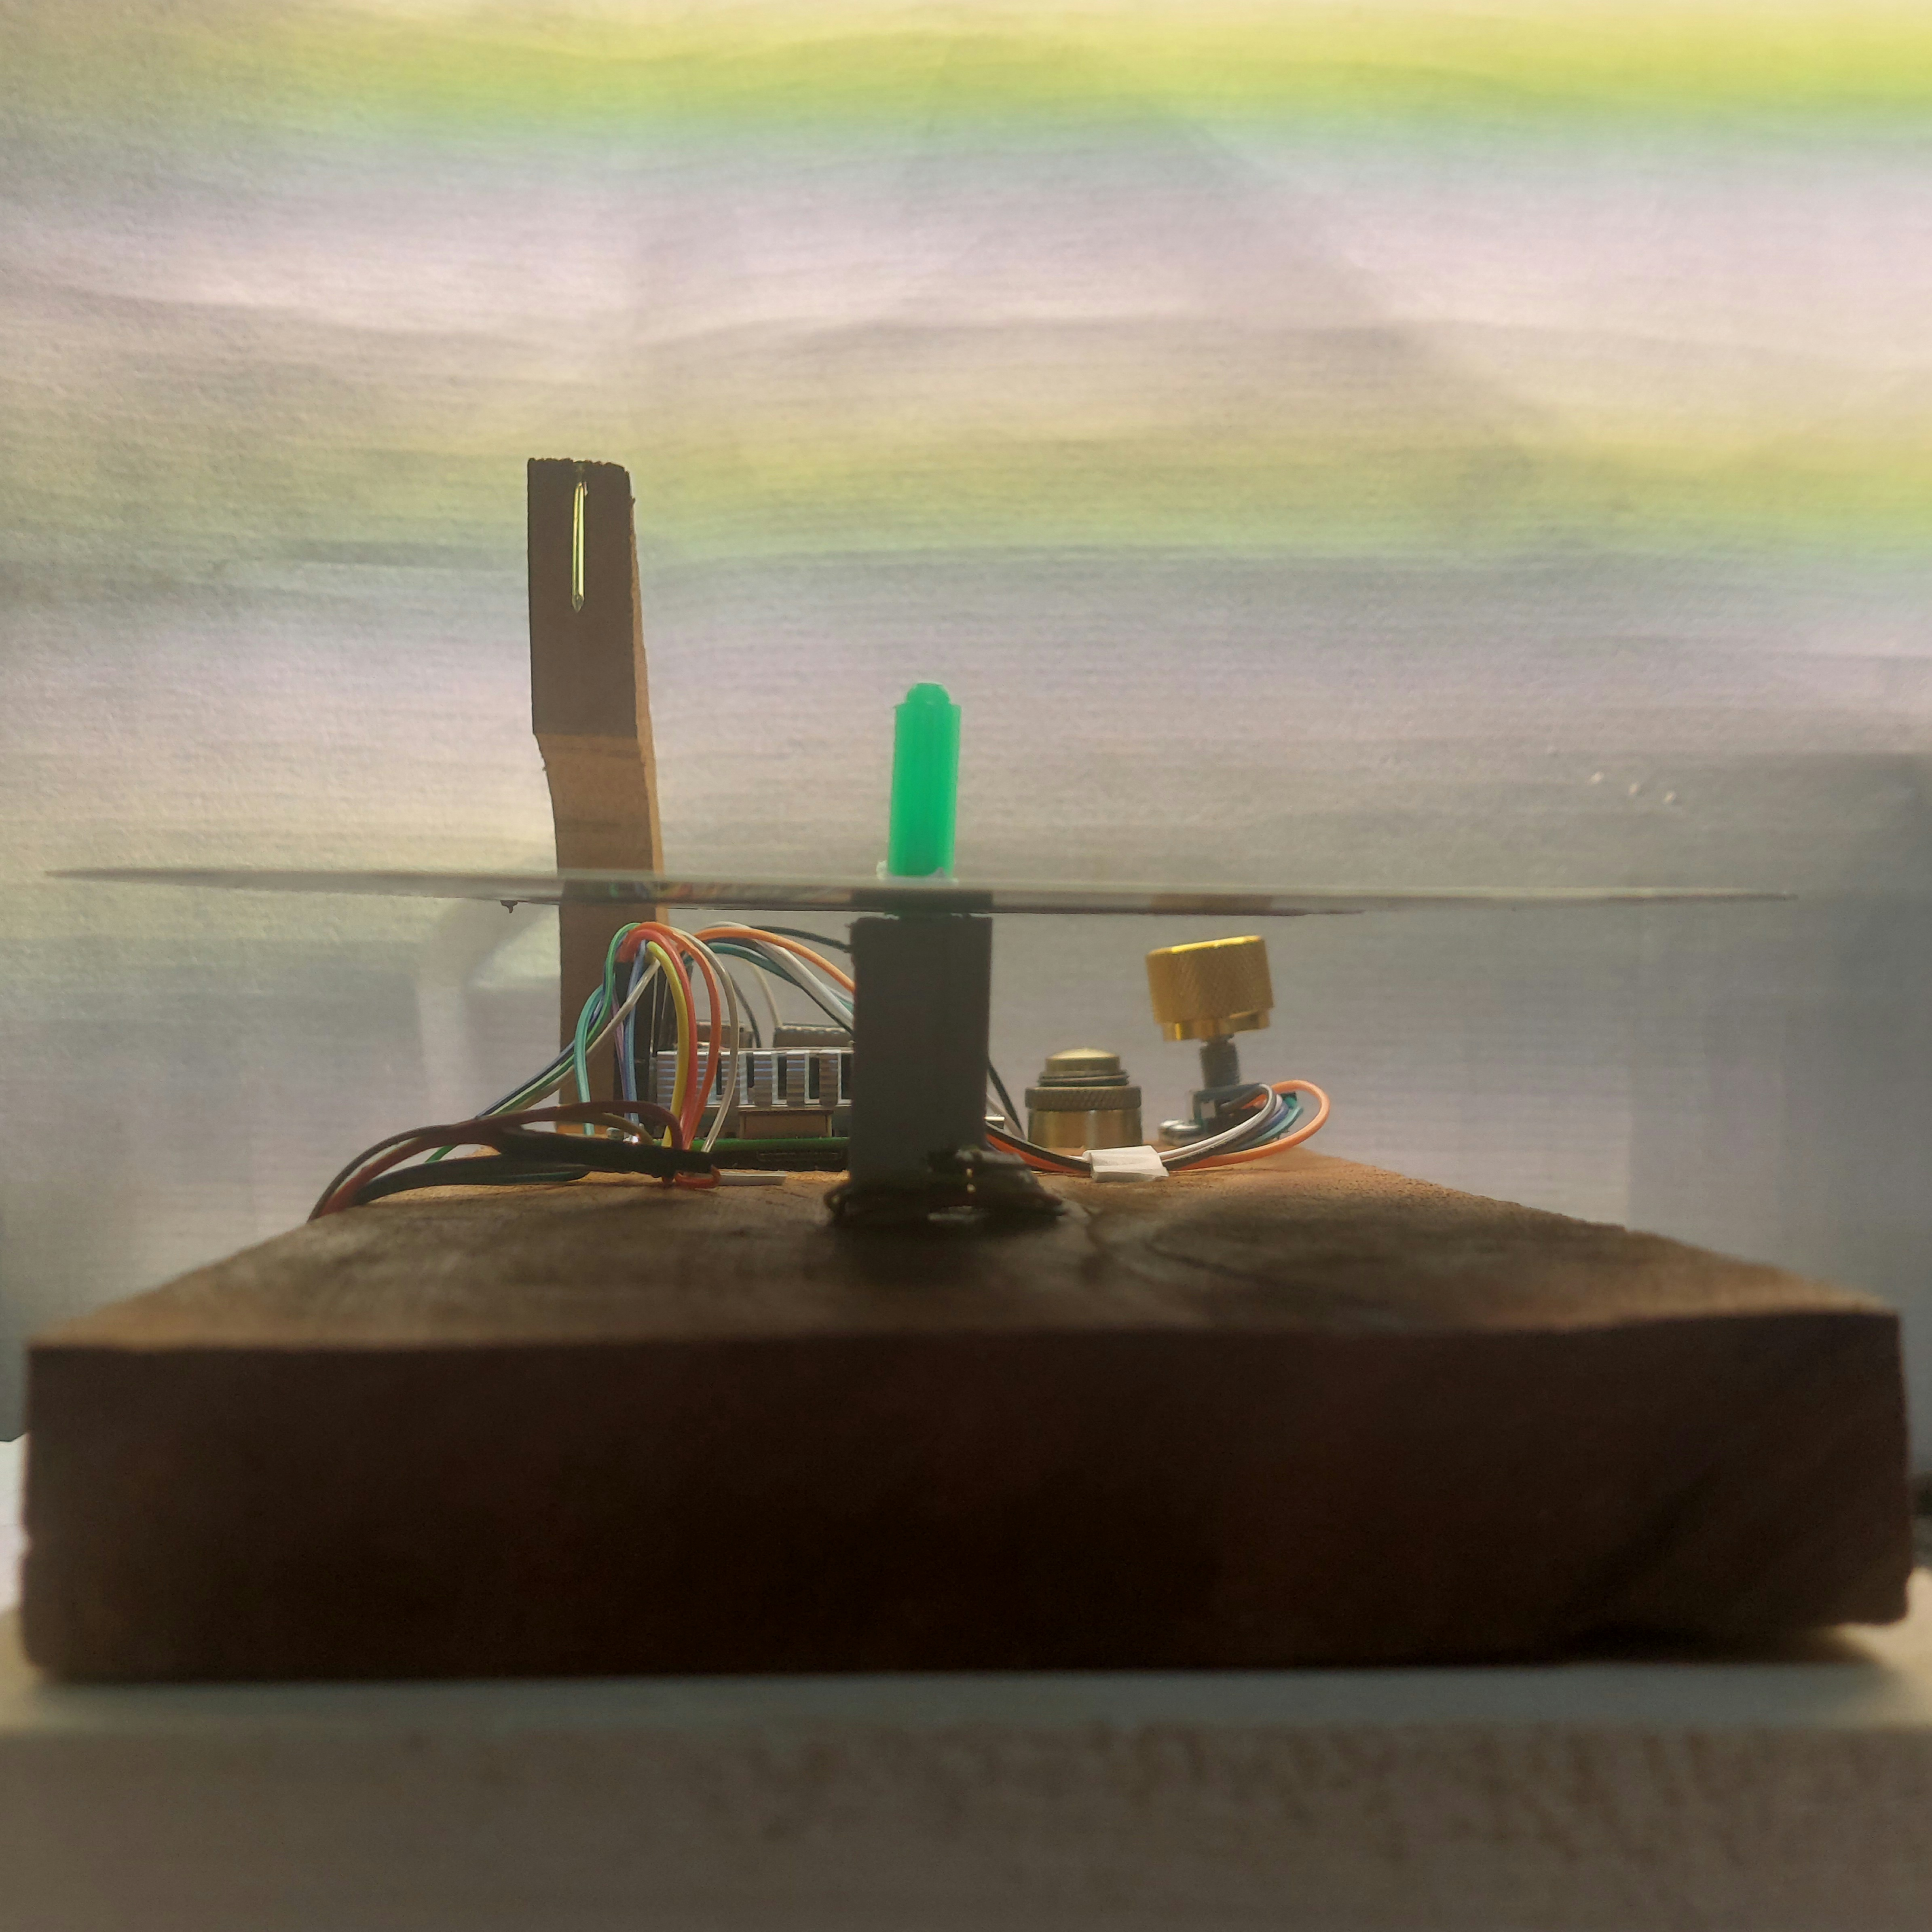
\includegraphics[width=\textwidth]{images/photos/profile_SIDE2.jpg}
                    \caption{`Far' side profile of the device}
                    \label{fig:side2}
                \end{minipage}
                \hfill
                \begin{minipage}[b]{0.45\textwidth}
                    \centering
                    \includegraphics[width=\textwidth]{images/photos/profile-BOTTOM.jpg}
                    \caption{Bottom-up profile of the device}
                    \label{fig:bottom}
                \end{minipage}
            \end{figure}
    
        \subsection{Integrated Hybrid System}
    
            Combining the above, the complete product functions as a fully standalone smart vinyl player. The projection-based host interface is displayed directly onto the disc surface during playback. The interface dynamically updates based on system state (e.g., track change, album detected) and user input.
    
            Figures~\ref{fig:wotw}–\ref{fig:colne} show the system in use,\footnote{Videos of the system are available at \url{https://youtu.be/t4fFDltrNjo}} including full interactive mode and the passive, minimal visual state.
    
            \begin{figure}[h]
                \centering
                \begin{minipage}[b]{0.45\textwidth}
                    \centering
                    \includegraphics[width=\textwidth]{images/photos/wotw-ui.jpg}
                \end{minipage}
                \hfill
                \begin{minipage}[b]{0.45\textwidth}
                    \centering
                    \includegraphics[width=\textwidth]{images/photos/wotw.jpg}
                \end{minipage}
                \caption{Front-end UI projected onto device, with interactive interface (left) and minimal interface (right).}
                \label{fig:wotw}
            \end{figure}
            
            \begin{figure}[h]
                \centering
                \begin{minipage}[b]{0.45\textwidth}
                    \centering
                    \includegraphics[width=\textwidth]{images/photos/colne-ui.jpg}
                \end{minipage}
                \hfill
                \begin{minipage}[b]{0.45\textwidth}
                    \centering
                    \includegraphics[width=\textwidth]{images/photos/colne-ui-zoom.jpg}
                \end{minipage}
                \caption{Front-end UI projected onto device, with full interactive interface.}
                \label{fig:colne}
            \end{figure}
    
    %%%%%%%%%%%%%%%%%% SECTION 6 %%%%%%%%%%%%%%%%%%
    \section{Evaluation} \label{sec:evaluation}
        % does it do what it is supposed to do?
        % how well?
        % how well against others?
    
        This section evaluates the system's effectiveness in meeting its goals, considering both quantitative performance and qualitative experience. Evaluation is divided into four areas: technical performance, user experience, comparison with existing workflows, and broader implications.
    
        Quantitative metrics include classification accuracy, metadata reliability, system responsiveness, and code robustness. Qualitative factors assess usability, aesthetics, and the hybrid nature of the physical and digital design. Finally, the system is compared against alternative methods, with discussion of limitations, trade-offs, and ethical considerations.
        
        \subsection{Quantitative Evaluation}
    
            \subsubsection{Album Classification Accuracy}
    
                To assess classification accuracy, the model was trained on the full dataset (\ref{data:aug} + \ref{data:val}) and evaluated on a held-out test set, \ref{data:trueTest}, of 34 images. It achieved a top-1 accuracy of 91.18\%, correctly predicting 31 out of 34 albums. Of the three errors, two were due to the model being trained on visually distinct variant covers (see Figure~\ref{fig:ModelEval}), with only one test image matching the training version. If these variant covers are treated as anomalies, the accuracy rises to 97.05\%. While the test set is relatively small and not exhaustive, it reflects a reasonable physical collection a user might own.
    
                \begin{figure}
                    \centering
                    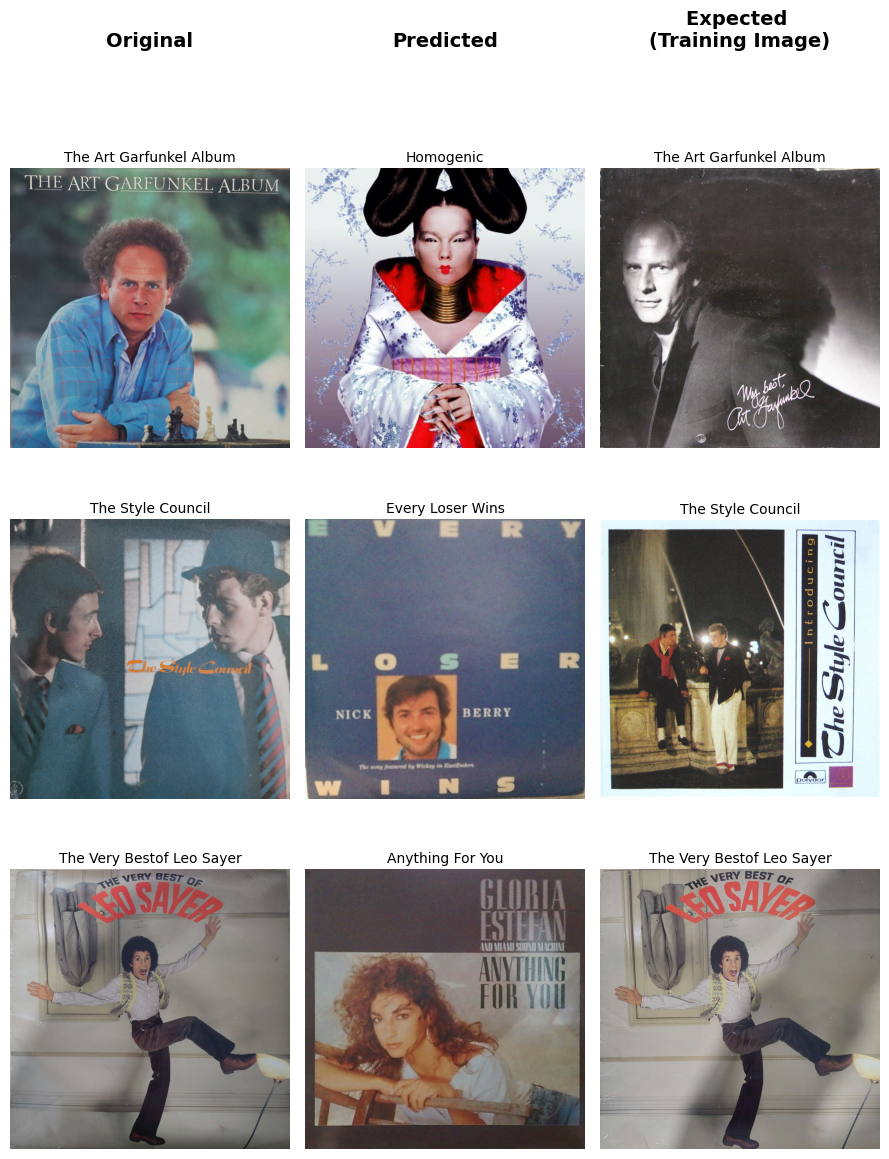
\includegraphics[width=0.5\linewidth]{images/modelEval.png}
                    \caption{Examples of misclassifications from the final test set}
                    \caption*{
                        Each row shows a failure case: the original input image (left), the model's incorrect prediction (centre), and the training image for the correct class (right). Errors primarily occured due to cover variants.
                    }
                    \caption*{
                        Artworks are © their respective copyright owners.
                    }
                    \label{fig:ModelEval}
                \end{figure}
    
                To mitigate poor classification, users can re-scan manually or upload a new image via a remote client. While fallback UI is minimal, the process remains low-friction, and improved lighting or positioning in the new image can help resolve earlier errors.
    
            \subsubsection{Metadata Retrieval Accuracy}
    
                Since metadata retrieval depends on external sources and network responses, evaluation was performed manually. A representative set of 32 albums was tested using automated centre-level retrieval. Of these, 4 were exact matches, 8 were correct but returned variant covers (e.g., CD editions), 2 matched the correct artist but wrong album, 15 returned no label, 2 returned unrelated images, and 1 returned an entirely incorrect label. In addition to the centre label, the Spotify album is also selected, which affects the textual metadata and album cover shown on remote devices. Of these same albums, 3 albums were compilations not present on Spotify, which led to retrievals of other compilations with similar themes (e.g., disco, Bond themes, Christmas). One album was a musical, correctly identified by title but with different performers, and one “best of” album was not available on Spotify, but yielded the correct artist. Despite some gaps, most queries retrieved results that were either correct or thematically relevant. With only a fairly low percentage of fetching bad data from Spotify (84.38\%; up to 96.88\% excluding compilations) the primary metadata source is correct, and as this only failed for particularly niche albums, a more standard collection should be very robust in the system.
    
                The centre label system was less reliable, yielding a relevant result in only 43.75\% of cases, with exact matches at 37.5\%. While suboptimal, it enhances visual context and remains acceptable due to its supplementary nature and the ability for users to override results by caching images manually. Nonetheless, future revisions to improve this pipeline would be beneficial.
    
            \subsubsection{System Responsiveness}
    
                Responsiveness was measured by timing the interval between user input (e.g., cover upload or classification trigger) and result delivery. The system was treated as an end-to-end pipeline. Tests across varying devices and network conditions showed average response times of under 2 seconds for classification and under 4 seconds for metadata retrieval, using the Ouroboros model trained on the full dataset. Worst-case latency occurred on slower connections, reaching up to 7 seconds. Overall, the system remained responsive and usable across typical usage scenarios.
    
            \subsubsection{Code Robustness}
    
                The codebase was evaluated through a suite of automated unit tests, covering core components such as image processing, metadata retrieval, and classification logic. The overall test pass rate is reported, and code coverage was estimated to ensure critical paths are exercised. No critical failures or regressions were observed during testing.
    
                The frontend achieved an average of 71.5\% statement coverage, with particularly strong performance in components like WebSocketManager.ts (96\%) and SpotifyPlayer.ts (92.4\%). The backend reached 66.2\% average coverage across core Python modules, with several key files such as sessionManager.py, stateManager.py, and modelHandler.py reaching very high coverages of 89–100\%. However, some components -- notably main.py, routes.py, and training utilities -- remain untested due to their hardware dependence or being out of scope.
                
                Overall, the combined project-wide coverage stands at 71.5\%, reflecting a strong foundation with room for expanding test coverage to the integration and hardware layers.
    
        \subsection{Qualitative Evaluation}
    
            To evaluate the emotional, aesthetic, and practical experience of the system, a user study was conducted with 17 participants. These users were surveyed after physically using the system, either through direct interaction or a guided session.
    
            Due to the nature of the device -- a physical prototype requiring in-person use -- there were significant constraints in recruiting participants. Access to the system was necessarily limited to those who could be reached directly, meaning the sample primarily consisted of friends, family, and peers. Additionally, many users only had brief interaction windows, limiting the depth of familiarity they could develop.
            
            This sample bias is acknowledged. There is likely a positive skew in the responses due to personal connection and the novelty of the system. That said, efforts were made to prompt critical feedback, and not all responses were favourable. While this limits generalisability, the feedback gathered still offers valuable insight into the usability, aesthetic reception, and conceptual strengths of the system.
    
            Feedback was collected via a structured Google Form following hands-on use of the system. The form included a combination of scaled questions and optional free-text responses, covering usability, satisfaction, convenience, and scanning accuracy. Responses also captured listening habits and attitudes toward physical media, providing broader context for interpreting user experience.
        
            \subsubsection{User Experience -- Usability}
                User testing focused on how intuitive the system felt to new users. Survey data from 17 participants showed a mostly positive trend:
                
                    76.5\% of users rated ease-of-use at 3 or higher,
                
                    with 35.3\% rating it 5 (very easy).
                    Only one user rated it as very difficult (1), citing a lack of initial instruction.
                
                Notable feedback highlighted the importance of a clear onboarding process, with one user commenting that ``the layout was good, but I didn't know what to do at first." Others praised its familiarity, especially those with vinyl experience, describing the interface as ``intuitive and natural."
                
                These results suggest that while the system is broadly accessible, it benefits significantly from prior exposure to analogue devices and would be improved by minimal visual guidance or prompts on first use.
    
            \subsubsection{User Experience -- Aesthetics}
                From the 17 responses, 70.6\% of participants who had experience with vinyl cited aesthetics as a key reason for ownership. This was reflected in comments such as ``felt more immersive than expected" and ``tactile feedback made it feel authentic."
    
                Design choices such as the use of real turntable elements, album art display, and the physical-digital hybrid interaction were positively received. Users described the system as ``satisfying to use" and ``visually rich."
                
                These findings indicate strong aesthetic engagement, aligning well with the nostalgic and cultural associations users have with vinyl.
            
        \subsection{Comparative Analysis}
            
            The system sits at the intersection of traditional vinyl playback and modern digital music access. Compared to standard streaming platforms, it introduces a tangible, physical interaction absent from purely digital interfaces. While streaming services offer convenience and breadth of access, they lack the ritual and aesthetic value that this system provides.
    
            In contrast to traditional record players, this system offers automatic metadata enrichment, playback synchronisation via Spotify, and album recognition -- features not available in analogue setups. However, it cannot match the audio fidelity on poor networks, or full physicality of actual vinyl playback.
            
            Compared to mobile apps that scan album covers (e.g., Shazam or Discogs), this system is less portable but more immersive. Its strength lies in offering a hybrid experience -- inviting physical interaction while integrating smart digital features.
    
            In informal benchmarks, this system's full album identification-to-playback cycle averaged $\approx 5.2$s. By contrast, Spotify search averages $\approx 4$s (but lacks physical input, and relied on existing user knowledge of the album details), while manual lookup via Discogs took over $\approx 20–30$s. Although slower than some pure-digital workflows, the hybrid interaction offers a richer, more deliberate experience.
    
        \subsection{Limitations and Trade-offs}
    
            A key limitation is the need for physical access to the system, which reduces scalability and reach. The classification model, while highly accurate on common albums, is less reliable on niche or variant covers. Metadata retrieval also depends on external APIs, and can produce incomplete or inaccurate results.
    
            From a technical standpoint, the system balances performance with simplicity, but lacks full robustness in edge cases (e.g., compilation albums or Spotify mismatches). Code coverage is strong but not complete, particularly around hardware-specific modules.
            
            There is also a trade-off between convenience and intentionality: while less convenient than streaming, the system offers a more deliberate and engaging listening experience -- by design.
    
        \subsection{Ethical Implications}
            
            This project prioritised ethical considerations throughout its lifecycle. Unlike generative AI systems, which often replicate or compete with original works, this classifier respects artistic integrity by not creating derivative content, nor redistributing copyrighted material.
            
            The system was designed to promote rather than replace physical media, aligning with the commercial interests of creators. Classification results are used solely to redirect users to legitimate playback platforms, potentially supporting royalties. No training data is exposed or accessible to users, and all datasets were acquired only from services explicitly permitting such use.
            
            Accessibility and openness were central goals -- with digital parity ensuring inclusive interaction, and full source availability supporting transparency and academic reuse. The project maintains a clear distinction between legal compliance and ethical responsibility, aiming to exceed beyond minimum standards in both.
    
    %%%%%%%%%%%%%%%%%% SECTION 7 %%%%%%%%%%%%%%%%%%
    \section{Conclusions and future work} % edit section heading as appropriate
        \subsection{Conclusions}
        % summarise results
    
            This project successfully met its core aims: building a fully functional hybrid media system that integrates physical interaction with digital music streaming (as shown in Tables~\ref{tab:FR}-\ref{tab:NFR}). Quantitative results showed strong model performance (91.18\% top-1 accuracy), fast response times (under 4s average), and solid code robustness (71.5\% coverage). Qualitative testing confirmed that users found the system intuitive and aesthetically engaging, with particular praise for its nostalgic design and physical-digital interaction.
    
            Limitations such as metadata inconsistency and edge-case classification were identified and mitigated where possible. User feedback revealed opportunities for clearer onboarding, but overall usability was high. Comparisons against existing tools underscored the novelty and experiential value of the system.
    
            \begingroup
                \renewcommand\thefootnote{}\footnotetext{Some deeper, yet more tangential thoughts are given in Appendix~\ref{sec:nailArt}, reflecting on the symbolic and aesthetic aspects of the system, beyond the scope of formal evaluation.}
                \addtocounter{footnote}{-1}
            \endgroup
    
        % achieved aims?
        \begin{longtable}{|c|p{5cm}|c|p{5cm}|}
            \caption{Evaluation of Functional Requirements} \label{tab:FR}\\
            \hline
            \textbf{ID} & \textbf{Requirement} & \textbf{Met?} & \textbf{Comment} \\
            \hline
            \endfirsthead
            \hline
            \textbf{ID} & \textbf{Requirement} & \textbf{Met?} & \textbf{Comment} \\
            \hline
            \endhead
            FR1 & Image recognition accuracy ≥90\% & Yes & Achieved 91.18\% top-1 accuracy (97.05\% if cover variants excluded). \\
            \hline
            FR2 & Playback initiation within 5 seconds & Yes & Average response time under 4 seconds; peak latency 7s on poor networks (initial assumptions included good connection). \\
            \hline
            FR3 & Integration with Spotify API & Yes & Functional integration achieved; metadata retrieved for 84.38\% of albums. \\
            \hline
            FR4 & Software playback controls & Yes & Users could reliably play/pause/skip tracks via the interface. \\
            \hline
            FR5 & Clear track/album information display & Yes & Displayed metadata from Spotify when available. \\
            \hline
            FR6 & Intuitive UI suitable for non-technical users & Yes & 76.5\% of users found it easy to use; onboarding could improve. \\
            \hline
            FR7 & Physical playback controls & Yes & Tactile controls implemented; users responded positively to physicality. \\
            \hline
        \end{longtable}
    
        \begin{longtable}{|c|p{5cm}|c|p{5cm}|}
            \caption{Evaluation of Non-Functional Requirements} \label{tab:NFR}\\
            \hline
            \textbf{ID} & \textbf{Requirement} & \textbf{Met?} & \textbf{Comment} \\
            \hline
            \endfirsthead
            \hline
            \textbf{ID} & \textbf{Requirement} & \textbf{Met?} & \textbf{Comment} \\
            \hline
            \endhead
            NFR1 & System latency ≤5 seconds & Yes & All processing within 4s on average; met under typical use. \\
            \hline
            NFR2 & System uptime ≥99\% & Yes & No runtime crashes observed in testing; highly stable during sessions. \\
            \hline
            NFR3 & Graceful handling of recognition failures & Partial & Errors redirected cleanly with fallback behaviour or retry prompts. Greater specificity in error messages could be improved. \\
            \hline
            NFR4 & Compatibility with Raspberry Pi 5 & Yes & Fully developed and deployed on Raspberry Pi 5 hardware. \\
            \hline
            NFR5 & Clear documentation for easy setup & Yes & Instructions and bash/batch scripts provided. \\
            \hline
            NFR6 & Compliance with UK copyright laws & Yes & Use justified under CDPA fair dealing \cite{cdpa1988}; no distribution of copyrighted media, beyond educational scope of report contents. \\
            \hline
            NFR7 (1) & Compliance with Spotify API Terms & Yes & Spotify data only used for playback; model training did not breach API terms. \cite{spotifyDevPolicy, spotifyDevTerms} \\
            \hline
            NFR7 (2) & Compliance with Discogs API Terms & Yes & Discogs data only fetched, cropped, and displayed; never fed into a model, did not breach API terms. \cite{discogsAPITOU, discogsToS} \\
            \hline
            NFR7 (3) & Compliance with Cover Art Archive API Terms & Yes & Data use limited to non-commercial research; metadata is CC0, and images are publicly accessible for educational use. \cite{coverartArchiveDoc} \\
            \hline
        \end{longtable}
    
        % improvements!
        
        \subsection{Future work}
          % ideas for further work
          % big ideas; what could be done with my project?
          Several directions exist for extending this project:
    
          \paragraph{Improving album detection with retraining and real-time augmentation}
    
          Whilst the Hydra expandable PNN model experiments were promising, they did not manage to mature into a usable production-grade state within the project's timespan. Future work into this model could be done to allow the system to be truly robust by allowing users to seamlessly add new albums to their collection, without losing performance quality.
    
          This could be taken even further, by enabling the system to learn from specific corrections made by users, improving classification over time, via reinforcement-trained updates based on user feedback.
    
          \paragraph{Onboarding and accessibility}
    
          Add minimal visual prompts, voice guidance, or mobile setup flows to improve ease-of-use for new users.
    
          \paragraph{Expanded integrations}
    
          Extend metadata sources to include lyrics, artist bios, or event listings, or connect fully to other streaming platforms, with the option to seamlessly switch between them on-the-fly (the current system requires manual re-configuration and rebooting of the server).
    
          \paragraph{Deeper HCI research}
    
           Conduct longer-term user studies focused on behaviour, nostalgia, and emotional connection to hybrid interfaces.
    
    %TC:ignore
    %%%%%%%%%%%%%%%%%% REFERENCES %%%%%%%%%%%%%%%%%%
    %\clearpage % uncomment to start on a new page if wanted
    \printbibliography[title={References},heading=bibintoc] % a single list of references for the whole thesis
    
    
    
    %%%%%%%%%%%%%%%%%% APPENDICES %%%%%%%%%%%%%%%%%%
    \begin{uomappendix} 
        % screen dumps of UI
        % important but large results
        \section{Project proposal}
    
            \begin{quote}
                Vinyl is back! According to the \href{https://www.nme.com/news/music/uk-vinyl-sales-2023-reach-highest-level-since-1990-3563676}{NME}, UK sales of vinyl in 2023 were the highest seen since 1990. Vinyl has always remained popular among niche genres, but we are also seeing mainstream artists like Taylor Swift and Lana Del Rey releasing and selling large volumes of albums on the format. Vinyl records have also recently been added into the ONS "Basket of Goods and Services": a carefully selected set of items representative of the goods and services that UK consumers typically spend their money on (\href{https://www.ons.gov.uk/news/news/arecordrevivalthatscookingupastormvinylmusicandairfryersspintheirwayintothebasketofgoods}{ONS}).
                
                Fans of the format claim better sound reproduction, with a fuller frequency range and a "warmth" lacking in digital formats such as CD. Playing vinyl requires specialist equipment: while the ritual of putting a disc on the turntable and dropping the needle is, for some, part of the experience, it can also be seen as an inconvenience.
                
                The aim of this project will be to develop an application that supports a blending of the physical and digital worlds. A physical artefact such as a Long Play (LP) is scanned using a camera. The information on the label or cover is then used to identify the release which can be played. This content could be retrieved from a streaming service such as Spotify or Apple Music, an artist site such as \href{https://bandcamp.com/}{Bandcamp}, or the user's own personal media library. This would then allow a user to "play" their records without a turntable. Although the audio quality may not match that of vinyl, such an application would appeal to those who like to collect vinyl for its own sake, or who appreciate the larger format artwork that comes with an old school LP. The application could run on a mobile phone or specialist hardware such as a Raspberry Pi equipped with a camera.
                
                Example methods that could be used for identification of the release include barcodes, QR codes or OCR acting on label text.
                
                For a stretch goal, the application could be extended to cover other media: the cassette tape (\href{https://www.theguardian.com/music/2023/apr/20/fun-way-consume-music-why-sales-of-cassette-tapes-soaring}{Guardian}) is also experiencing a comeback, although the \href{https://en.wikipedia.org/wiki/8-track_cartridge}{eight-track} is unlikely to be retrieved from the dustbin of history.
                
                The project should be considered as challenging. It will require integration of several technologies and some creativity.
            \end{quote}
    
            Written by Sean Bechhofer. \cite{bechhofervttspec}.
        
        \section{Risk register}
            
            \begin{longtable}{|c|p{3.2cm}|c|c|p{4.1cm}|p{3.0cm}|}
                \caption{Project Risk Register} \label{tab:riskRegister} \\
                
                \hline
                \textbf{ID} & \textbf{Risk Description} & \textbf{Likelihood} & \textbf{Impact} & \textbf{Mitigation Strategy} & \textbf{Status} \\ \hline
                \endfirsthead
                
                \hline
                \textbf{ID} & \textbf{Risk Description} & \textbf{Likelihood} & \textbf{Impact} & \textbf{Mitigation Strategy} & \textbf{Status} \\ \hline
                \endhead
    
                R1 & Legal issues with dataset use (e.g., image rights) & Low & High & Use open-licensed datasets only (e.g., Cover Art Archive); delete images post-training & Avoided \\ \hline
                R2 & API deprecation or change & Low & High & Use modular, abstracted API interfaces; track API updates; prepare fallback providers & Occurred (Spotify callback HTTPS requirement) -- mitigated \\ \hline 
                R3 & API or service outage (or rate limiting) & Medium & High & Pre-cache training data; shortlist backup sources (e.g., Last.fm) & Occurred (Internet Archive downtime) -- mitigated \\ \hline
                R4 & GPIO hardware failure (e.g., fried pin) & Medium & Medium & Use spare GPIO pins; include pin redundancy in design & Occurred -- mitigated \\ \hline
                R5 & Training model on Pi is too slow or infeasible & High & Medium & Perform training externally; retain inference compatibility with Pi & Occurred -- resolved \\ \hline
                R6 & Inaccessible interface for some users & Medium & Medium & Provide remote access UI; physical + digital controls; customisable projection settings & Addressed \\ \hline
                R7 & Security flaw in remote access & Low & High & Use session validation; limit access to LAN; restrict command permissions & Mitigated \\ \hline
                R8 & Performance throttling (e.g., heat) & Medium & Medium & Use active cooling; monitor CPU load & Occurred -- resolved \\ \hline
                R9 & DRM compatibility issues on ARM devices & High & High & Use official Widevine build; switch to alternative hardware if required & Occurred -- resolved \\ \hline
                R10 & Compatibility issues across browsers & Low & Medium & Test on multiple browsers; prefer standards-compliant tools (e.g., React, FastAPI) & Monitored \\ \hline
            \end{longtable}
    
        \section{Model Cards} \label{sec:mcard}
        
            \paragraph{Ouroboros}
    
                \url{https://github.com/Razzula/virtual-turntable/blob/main/server/modelling/models/models/Ouroboros/model-card.md}
        
                \lstinputlisting[
                    language=markdown,
                    caption={Ouroboros Model Card.},
                    label={lst:ouro}
                ]{code/ModelCard.md}
            
            \paragraph{Baby Ouroboros}
        
                \url{https://github.com/Razzula/virtual-turntable/blob/main/server/modelling/models/models/BabyOuroboros/model-card.md}
        
            \paragraph{Amphisbaena}
        
                \url{https://github.com/Razzula/virtual-turntable/blob/main/server/modelling/models/models/Amphisbaena/model-card.md}
        
            \paragraph{Hydra}
        
                As no production form of the Hydra model was made, there is therefore no output model available, and so does not have a model card.
        
                The experimentation, however, can be seen at \url{https://github.com/Razzula/virtual-turntable/blob/main/server/modelling/sandbox/RetrainableCNN.ipynb}.
    
        \section{Datasets}
    
            \begin{figure}[H]
                \centering
                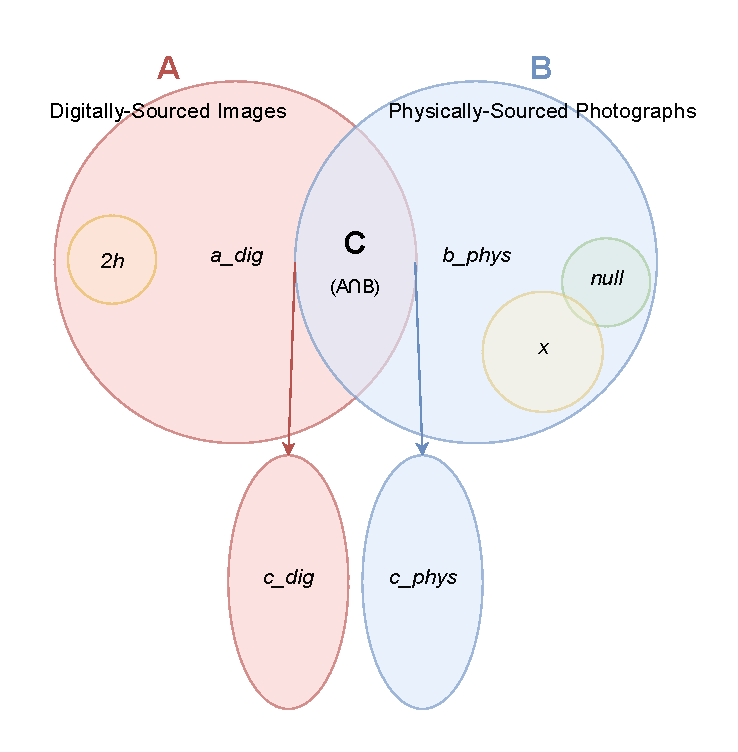
\includegraphics[width=0.6\textwidth]{images/DataVenn.pdf}
                \caption{Overview of dataset partitioning by source and subset.}
                \label{fig:dataVenn}
            \end{figure}
    
            Figure~\ref{fig:dataVenn} shows the full dataset, grouped by source origin (digital or physical), and its partitioning into training, validation, and test sets, along with the subset relationships. Sections~\ref{data:null}.0--\ref{data:trueTest} provide a detailed breakdown of the precise subsets used in model development and training, including full summaries of their contents and sources, in line with best practices for open, transparent, and reproducible research \cite{Mitchell_2019}.
    
            \subsection*{D.0\quad Null Data} \label{data:null}
    
                This set consists of a single data point\footnote{\url{https://github.com/Razzula/virtual-turntable/blob/main/server/modelling/data/art_/_null/_null/null.jpg}} representing the \textit{null} class-- an explicit placeholder used to represent unknown or unclassified inputs. It was manually included for baseline calibration and failure case testing.
    
            \subsection{Training Set `Mini'} \label{data:mini}
    
                This compact set includes:
                \begin{itemize}
                    \item The \textit{null} class (\ref{data:null}),
                    \item +11 digitally-sourced albums (+20 image samples; partition of \texttt{a\_dig}),
                \end{itemize}
    
                21 image samples, for 12 classes, in total.
    
                Used for early-stage prototyping and model shaping. The full list of albums included are listed in the manifest.\footnote{\url{https://github.com/Razzula/virtual-turntable/blob/cb3e1561de8f4f9d98f850b8b971f118cdb5e25c/server/modelling/data/manifest.json}}
    
            \subsection{Training Set `Large'} \label{data:large}
    
                This is the main full-scale training set, consisting of:
                \begin{itemize}
                    \item All data from \ref{data:mini},
                    \item +58 digitally-sourced albums (+113 samples; \texttt{a\_dig}),
                    \item +20 physically-sourced albums (+39 samples; \texttt{b\_phys}),
                    \item +13 albums\footnote{14 classes were included, but one (Jeff Wayne's \textit{War of the Worlds}) overlaps with \ref{data:mini}.} with both digital and physical variants (+23 samples; \texttt{c\_dig}).
                \end{itemize}
    
                196 image samples, for 103 classes, in total.
                
                The full list of albums used are listed in the repository.\footnote{\url{https://github.com/Razzula/virtual-turntable/blob/63f087f36f2dacd62cf51ccb8731cc891d10850c/server/modelling/data/albums.json}}
    
            \subsection{Training Set Augmented} \label{data:aug}
    
                This dataset builds on \ref{data:large} with online data augmentation:
                \begin{itemize}
                    \item Augmentations are applied randomly per-epoch,
                    \item Effective dataset size is increased by a factor of five,
                    \item Transformations include colour jitter, rotation, blur, and noise, as shown in Listing~\ref{lst:aug}
                \end{itemize}
    
                1176 image samples, for 103 classes, in total.
    
                \lstinputlisting[
                    language=Python,
                    caption={Data augmentation transformatons.},
                    label={lst:aug}
                ]{code/Transforms.py}
    
            \subsection{Validation Set} \label{data:val}
    
                This set includes:
                \begin{itemize}
                    \item 14 albums,
                    \item 16 samples,
                    \item All data from the \texttt{c\_phys} subset.
                \end{itemize}
    
                Each entry is a physically-sourced photograph of an album also represented digitally in \texttt{c\_dig}, making this set useful for assessing model generalisation.
                
                The list of albums included is available in the repo.\footnote{\url{https://github.com/Razzula/virtual-turntable/blob/644358e3a9591f28d912af3c5dce7ad9e7b49754/server/modelling/data/albums_phys.json}}
    
            \subsection{Challenge Set} \label{data:test}
    
                This dataset expands on the validation set by further including physically augmented samples of albums (extreme lighting, rotation, motion blur), with the intention of being very hard to classify.
    
                Figure~\ref{fig:dataTest} shows a sample of this dataset, with the left-most image being the standard training image (from \texttt{b\_phys}), and the others being extreme test cases (essentially, `bad data').
    
                \begin{figure}[H]
                    \centering
                    \includegraphics[width=\linewidth]{images/ChallengeData.png}
                    \caption{Training image of album (left), alongside physically augmented variants for generalisation testing.}
                    \label{fig:dataTest}
                    \caption*{Includes artwork from \textit{Comrades In Song} (1970) by Colne Valley Male Voice Choir. Used for non-commercial research purposes under fair dealing.}
                \end{figure}
    
                \begin{itemize}
                    \item All data from \ref{data:val},
                    \item +1 \texttt{null} class entry (4 samples),
                    \item +16 physically-sourced samples across existing classes,
                    \item Includes hard-mode variants (e.g., low lighting, motion blur).
                \end{itemize}
    
                36 image samples, for 15 classes, in total.
    
            \subsection{Multi-Head Test Set} \label{data:test2}
    
                This specialised set builds upon \ref{data:test}, adding:
                \begin{itemize}
                    \item +1 unseen class: \textit{2h},\footnote{Album: − (Subtract), Ed Sheeran (2023).}
                    \item +2 unique data points.
                \end{itemize}
    
                Used to evaluate multi-class expansion handling, especially by the Amphisbaena and Hydra architectures.
    
            \subsection{Unseen Test Set}\label{data:trueTest}
    
                This set comprises:
                \begin{itemize}
                    \item 34 classes,
                    \item 34 samples (front covers only),
                    \item Corresponding to the albums in the \texttt{c\_phys} and \texttt{b\_phys} subsets.
                \end{itemize}
    
                All images were newly captured photographs of the same physical albums in \texttt{c\_phys} and \texttt{b\_phys}, taken in a different location, under different lighting conditions, using a different camera than those in the training set. No attempts were made to eliminate artefacts such as glare or shadows. This dataset simulates realistic, uncontrolled inputs of a small home collection and was reserved exclusively for formal evaluation.
    
        \section{Evaluation Results}
    
            \subsection{Unit Tests}
                % \paragraph{Front End}
                \begin{table}[H]
                    \centering
                    \caption{Front-end unit test coverage output (Vitest)}
                    \begin{verbatim}
    -----------------------|---------|----------|---------|---------|
    File                   | % Stmts | % Branch | % Funcs | % Lines |
    -----------------------|---------|----------|---------|---------|
    All files              |    71.5 |    81.81 |   58.71 |    71.5 |
     src                   |   76.76 |    82.08 |   47.27 |   76.76 |
      App.tsx              |   58.64 |    90.24 |   33.33 |   58.64 |
      RemoteController.tsx |   77.91 |    82.85 |      30 |   77.91 |
      VirtualTurntable.tsx |   84.65 |     75.9 |   40.74 |   84.65 |
      WebSocketManager.ts  |      96 |      100 |    90.9 |      96 |
      root.tsx             |       0 |        0 |       0 |       0 |
     src/APIs              |    42.1 |      100 |      60 |    42.1 |
      IMusicAPI.ts         |       0 |        0 |       0 |       0 |
      IMusicPlayer.ts      |    42.1 |      100 |      50 |    42.1 |
     src/APIs/Local        |       3 |        0 |       0 |       3 |
      LocalPlayer.ts       |       3 |        0 |       0 |       3 |
     src/APIs/Spotify      |   76.47 |    94.11 |   72.72 |   76.47 |
      SpotifyAPI.ts        |    66.4 |    92.85 |   66.66 |    66.4 |
      SpotifyPlayer.ts     |    92.4 |       95 |   76.92 |    92.4 |
     src/common            |   72.05 |    66.66 |   70.83 |   72.05 |
      Dialogue.tsx         |    56.6 |     62.5 |   66.66 |    56.6 |
      Tooltip.tsx          |   79.25 |    46.15 |    62.5 |   79.25 |
      WebcamCapture.tsx    |   78.78 |    86.66 |      80 |   78.78 |
     src/types             |     100 |      100 |     100 |     100 |
      Music.ts             |       0 |        0 |       0 |       0 |
      vendor.ts            |     100 |      100 |     100 |     100 |
     src/utils             |     100 |      100 |     100 |     100 |
      blob.ts              |     100 |      100 |     100 |     100 |
    -----------------------|---------|----------|---------|---------|
                    \end{verbatim}
                \end{table}
    
                % \paragraph{Back End}
                \begin{table}
                    \centering
                    \caption{Back-end unit test coverage output (Pytest)}
                    \begin{verbatim}
    Name                                          Stmts   Miss  Cover
    -----------------------------------------------------------------
    app\APIs\DiscogsAPI.py                           49      2    96%
    app\APIs\MusicAPI\IMusicAPI.py                   47     13    72%
    app\APIs\MusicAPI\SpotifyAPI.py                 132     61    54%
    app\enums\StateKeys.py                           16      0   100%
    app\main.py                                     182    182     0%
    app\modules\Hardware\IHardwareController.py      31      9    71%
    app\modules\Hardware\piController.py            149    130    13% 
    app\modules\centreLabelHandler.py                70     11    84% 
    app\modules\modelHandler.py                      70      7    90%
    app\modules\sessionManager.py                    48      0   100%
    app\modules\stateManager.py                      35      4    89%
    app\modules\websocketHandler.py                  55     43    22%
    app\routes.py                                   161    161     0%
    app\utils.py                                     35      8    77%
    modelling\__init__.py                             0      0   100%
    modelling\getAlbumArt.py                        131    131     0%
    modelling\models\Amphisbaena.py                 127    109    14%
    modelling\models\BabyOuroboros.py                22     14    36%
    modelling\models\Ouroboros.py                   107     89    17%
    modelling\models\__init__.py                      0      0   100%
    modelling\models\train.py                        87     87     0%
    modelling\models\utils\CustomDataset.py         100     80    20%
    modelling\models\utils\ModelType.py               5      0   100%
    modelling\models\utils\RandomFlip.py             12      4    67%
    modelling\models\utils\Transforms.py              4      0   100%
    modelling\models\utils\__init__.py                0      0   100%
    -----------------------------------------------------------------
                    \end{verbatim}
                \end{table}
    
            \subsection{System Evaluation}
                % \paragraph{Ouroboros Model} \\
    
                \begin{adjustbox}{max width=\textwidth}
                    \begin{lstlisting}[caption={Ouroboros model evaluation results on test set \ref{data:trueTest} (34 images)}, label={lst:ourobEval}]
    Evaluation Results:
    Total images evaluated: 34
    Correct predictions: 31
    Accuracy: 91.18%
    
    Failures:
    TheArtGarfunkelAlbum_ArtGarfunkel_1984 (Homogenic_Björk_1997)
    TheStyleCouncil_TheStyleCouncil_1983 (EveryLoserWins_NickBerry_1986)
    TheVeryBestofLeoSayer_LeoSayer_1979 (AnythingForYou_GloriaEstefanandMiamiSoundMachine_1988)
                    \end{lstlisting}
                \end{adjustbox}
    
        \section{Image Overflow} \label{app:img}
    
            \begin{figure}[htbp]
                \centering
                \includegraphics[width=\linewidth]{images/Amphisbanae.pdf}
                \caption{Architecture for Amphisbanae model (ResNet18 dual-classifier).}
                \label{fig:AmphisbanaeCNN}
            \end{figure}
    
            \begin{figure}[H]
                \centering
                \begin{minipage}[b]{0.45\textwidth}
                    \centering
                    \includegraphics[width=\textwidth]{images/screenshots/HOST_Auth.png}
                    \caption{Screenshot of host client using Spotify's authentication redirection flow}
                    \label{fig:hostAuth}
                \end{minipage}
                \hfill
                \begin{minipage}[b]{0.45\textwidth}
                    \centering
                    \includegraphics[width=\textwidth]{images/screenshots/HOST_Cam.png}
                    \caption{Screenshot of host client displaying the input image from the camera}
                    \label{fig:hostCam}
                \end{minipage}
            \end{figure}
                
            \begin{figure}[H]
                \centering
                \begin{minipage}[b]{0.45\textwidth}
                    \centering
                    \includegraphics[width=\textwidth]{images/screenshots/HOST_Green.png}
                    \caption{Screenshot of host client using adaptive colouring and texturing}
                    \label{fig:hostGreen}
                \end{minipage}
                \hfill
                \begin{minipage}[b]{0.45\textwidth}
                    \centering
                    \includegraphics[width=\textwidth]{images/screenshots/LAPTOP_Cam.png}
                    \caption{Screenshot of a remote client (PC) using the camera functionality}
                    \label{fig:laptopCam}
                \end{minipage}
            \end{figure}
                
            \begin{figure}[H]
                \centering
                \begin{minipage}[b]{0.45\textwidth}
                    \centering
                    \includegraphics[width=\textwidth]{images/screenshots/LAPTOP_External.png}
                    \caption{Screenshot of a remote client, using an external account (not the host)}
                    \label{fig:laptopExternal}
                \end{minipage}
            \end{figure}
            
            \begin{figure}[H]
                \centering
                \begin{minipage}[b]{0.45\textwidth}
                    \centering
                    \includegraphics[width=\textwidth]{images/screenshots/PHONE_Cam.jpg}
                    \caption{Screenshot of a remote client (mobile) using the camera functionality}
                    \label{fig:phoneCam}
                \end{minipage}
                \hfill
                \begin{minipage}[b]{0.45\textwidth}
                    \centering
                    \includegraphics[width=\textwidth]{images/screenshots/PHONE_Error.jpg}
                    \caption{Screenshot of a remote client displaying a 404 error}
                    \label{fig:phoneError}
                \end{minipage}
            \end{figure}
    
        \section{Supplementary Information}
    
            \subsection{Mythological Inspiration} \label{app:Greek}
    
                \paragraph{Ouroboros} A mythological serpent known for circling and eating its own tail, as in Figure~\ref{fig:ouroboros}. This name was used for the simple one-headed CNN model design, which `self-fed' on deployment data with a low-distribution shift between its training data.
    
                \paragraph{Amphisbaena} A snake-like creature, also of origin in Greek mythology, with a notable second head at the end of its tail, as in Figure~\ref{fig:amphisbaena}. This creature's name was used for the two-headed neural network design.
    
                \paragraph{Hydra} A rather famous mythological Greek monster, the Hydra of Lerna is a serpentine lake monster, famed for having many heads. These carying number of heads are most well-known for the fact that for every one that was cut off, two more would re-grow in its place. This creature's name was used for the PNN model design, which featured a growing number of heads.
    
                \begin{figure}[h]
                    \centering
                    \includegraphics[width=0.6\textwidth]{images/Ouroborus.jpg}
                    \caption{A drawing of an ouroboros, in an alchemical tract (1478)}
                    \label{fig:ouroboros}
                    \caption*{Source: \href{https://en.wikipedia.org/wiki/File:Serpiente_alquimica.jpg}{Wikipedia}}
                \end{figure}
    
                \begin{figure}[H]
                    \centering
                    \includegraphics[width=0.6\textwidth]{images/Amphisbaena.png}
                    \caption{An illustration of an amphisbaena}
                    \label{fig:amphisbaena}
                    \caption*{Source: \href{https://www.abdn.ac.uk/bestiary/ms24/f68v}{The Aberdeen Bestiary, folio 68V (c. 1200).}}
                \end{figure}
    
            \subsection{Cultural Inspiration} \label{app:Cult}
    
                \paragraph{Ed Sheeran Meme} As a light-hearted cultural reference, a meme (Figure~\ref{fig:EdMeme}) highlighting the uniformity of Ed Sheeran's album art served partially as inspiration for designing an artist classifier. The visual similarity in album covers suggested that artist and album may be decoupled yet jointly learnable.
    
                \begin{figure}[H]
                    \centering
                    \includegraphics[width=0.6\textwidth]{images/EdSheeranMeme.jpg}
                    \caption{A social media post jokingly referencing the consistent visual theme of Ed Sheeran's album covers}
                    \label{fig:EdMeme}
                    \caption*{Source: \href{https://www.threads.net/@pun_bible/post/DB83pw3gZSh/media}{\@pun\_bible (threads.net)}}
                \end{figure}
    
        \section{Ponderings on what the project expresses} \label{sec:nailArt}
    
        At the centre of this system lies a single vinyl disc (see Figure~\ref{fig:product}), fixed in place. It serves no functional role in audio playback, but instead acts as a blank canvas -- spinning beneath a projector that overlays metadata and centre-label imagery. The user's actual records are never played, only scanned via their sleeves, preserving them entirely. This one disc, however, is not so fortunate.
    
        A nail, mounted in place of a stylus, crudely scratches against the rotating surface. Though mechanically redundant, it produces a faint scraping sound -- evoking the familiar hiss of analogue playback. Ironically, this unintended acoustic artefact became central to the experience: an authentic, physical sound that reinforces the illusion of vinyl, even as the music itself is streamed digitally. Yet the sound emitted is, in fact, the destruction of the vinyl's own grooves -- the very data it once held, gradually scraped away.
        
        What began as a visual flourish now feels almost symbolic. The system preserves physical media, yet requires one record to be worn down in the process. A vinyl that exists purely to look like any vinyl, its own centre label concealed beneath a blank white sheet to be projected upon in mimicry; and to sound like a generic vinyl -- forced to scrape and screech, but not its own original composition, which is instead destroyed with each rotation. In retrospect, it's a strange reversal: a digital player that needs physical damage to feel more analogue. A disc slowly degrading under a metal point to lend authenticity to a digital experience.
        
        None of the user's own records are harmed, yet this one sacrificial vinyl remains essential. It makes no contribution to the music, yet is critical to the illusion. It is not played, but must still be heard -- not for the value of what it once held, but for what it now represents.
        
        There is something both comical and oddly poetic in this inversion: a system that digitises collections, yet requires a physical artefact to feel analogue. In hindsight, this unintentional arrangement reflects a curious tension -- between preservation and performance, where simulation relies on the very thing it seeks to replace.
        
        %\section{Other appendices as necessary}
    \end{uomappendix}
    
    
    %%%%%%%%%%%%%%%%%% END MATTER %%%%%%%%%%%%%%%%%%
    %TC:endignore
    \end{document}